\chapter{Machin Learning Results}
\section{Timeout instances}

\label{sec:annexe:timeout_instances}

\begin{table}[h]
\centering
\begin{tabular}{ll}
\hline
dataset & instance \\ 
\hline
25\_filtered\_chunk\_extraction\_-e\_none\_-s\_activate & Transformers 0 \\ 
25\_filtered\_chunk\_extraction\_-e\_none\_-s\_activate & Transformers 1 \\ 
26\_filtered\_chunk\_extraction\_-e\_only-max-entropy\_-s\_none & Transformers 2 \\ 
26\_filtered\_chunk\_extraction\_-e\_only-max-entropy\_-s\_none & Transformers 3 \\ 
26\_filtered\_chunk\_extraction\_-e\_only-max-entropy\_-s\_none & Transformers 4 \\ 
26\_filtered\_chunk\_extraction\_-e\_only-max-entropy\_-s\_none & Transformers 5 \\ 
26\_filtered\_chunk\_extraction\_-e\_only-max-entropy\_-s\_none & Transformers 6 \\ 
26\_filtered\_chunk\_extraction\_-e\_only-max-entropy\_-s\_none & Transformers 7 \\ 
\hline
\end{tabular}
\caption{Timeouts instances}
\label{tab:timeouts}
\end{table}

\section{Feature engineering fails}

\label{sec:annexe:feature_engineering_fails}

The list is empty.

\section{Feature Engineering results}

\label{sec:annexe:feature_engineering_results}

\subsection{26\_filtered\_chunk\_extraction\_-e\_only-max-entropy\_-s\_none}

\begin{longtable}{|c|c|}
\caption{Transformers 0 Feature Engineering Results on 26\_filtered\_chunk\_extraction\_-e\_only-max-entropy\_-s\_none} \label{tab:26_filtered_chunk_extraction_-e_only-max-entropy_-s_none_transformers_0_feature_engineering_results}\\
\hline
Dataset Name & 26\_filtered\_chunk\_extraction\_-e\_only-max-entropy\_-s\_none \\ \hline
Instance & Transformers 0 \\ \hline
\multirow{8}{*}{Best Features} & embedded\_6 \\ \cline{2-2}
 & embedded\_3 \\ \cline{2-2}
 & embedded\_0 \\ \cline{2-2}
 & embedded\_5 \\ \cline{2-2}
 & embedded\_4 \\ \cline{2-2}
 & embedded\_1 \\ \cline{2-2}
 & embedded\_2 \\ \cline{2-2}
 & embedded\_7 \\ \cline{2-2}
\noalign{\vskip 5mm}
\multicolumn{2}{|c|}{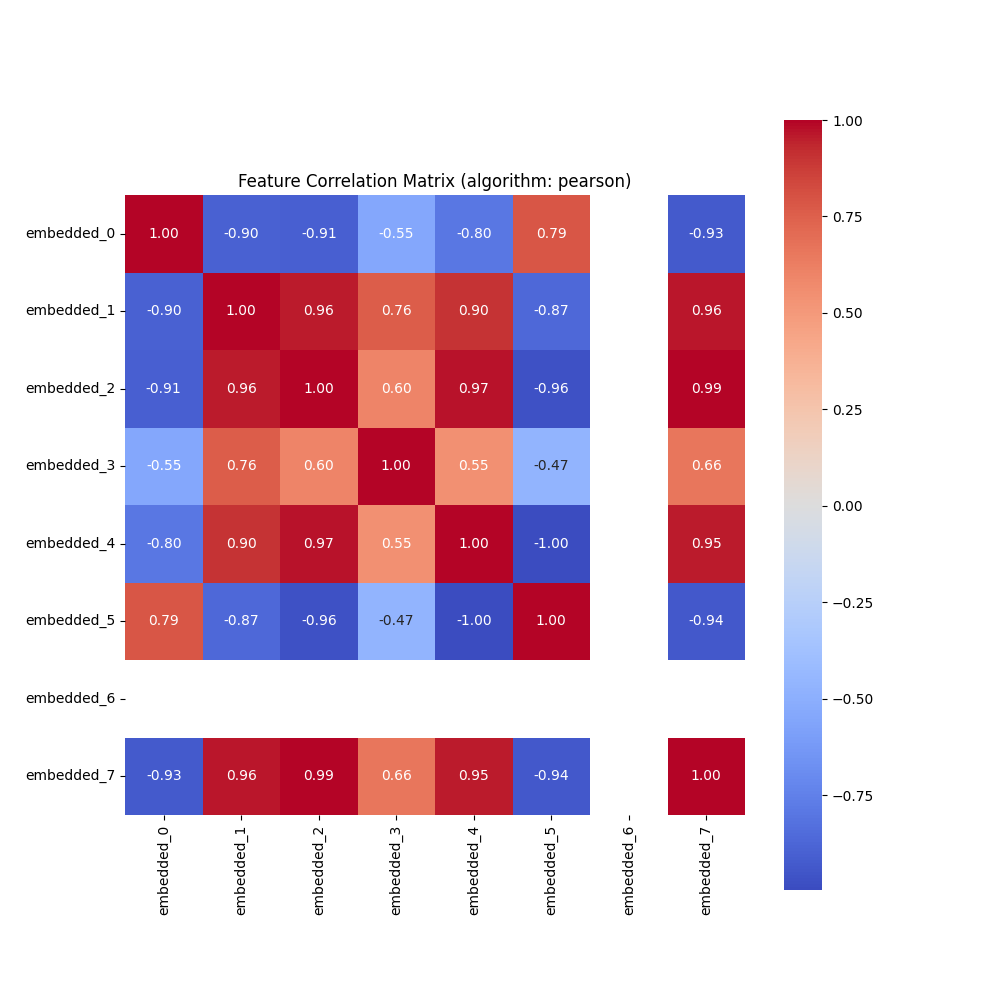
\includegraphics[width=0.8\linewidth]{img/annexes/26_filtered_chunk_extraction_-e_only-max-entropy_-s_none/Transformers 0_correlation_matrix.png}} \\
\hline
\end{longtable}


\begin{longtable}{|c|c|}
\caption{Transformers 1 Feature Engineering Results on 26\_filtered\_chunk\_extraction\_-e\_only-max-entropy\_-s\_none} \label{tab:26_filtered_chunk_extraction_-e_only-max-entropy_-s_none_transformers_1_feature_engineering_results}\\
\hline
Dataset Name & 26\_filtered\_chunk\_extraction\_-e\_only-max-entropy\_-s\_none \\ \hline
Instance & Transformers 1 \\ \hline
\multirow{8}{*}{Best Features} & embedded\_2 \\ \cline{2-2}
 & embedded\_8 \\ \cline{2-2}
 & embedded\_14 \\ \cline{2-2}
 & embedded\_5 \\ \cline{2-2}
 & embedded\_6 \\ \cline{2-2}
 & embedded\_1 \\ \cline{2-2}
 & embedded\_13 \\ \cline{2-2}
 & embedded\_15 \\ \cline{2-2}
\noalign{\vskip 5mm}
\multicolumn{2}{|c|}{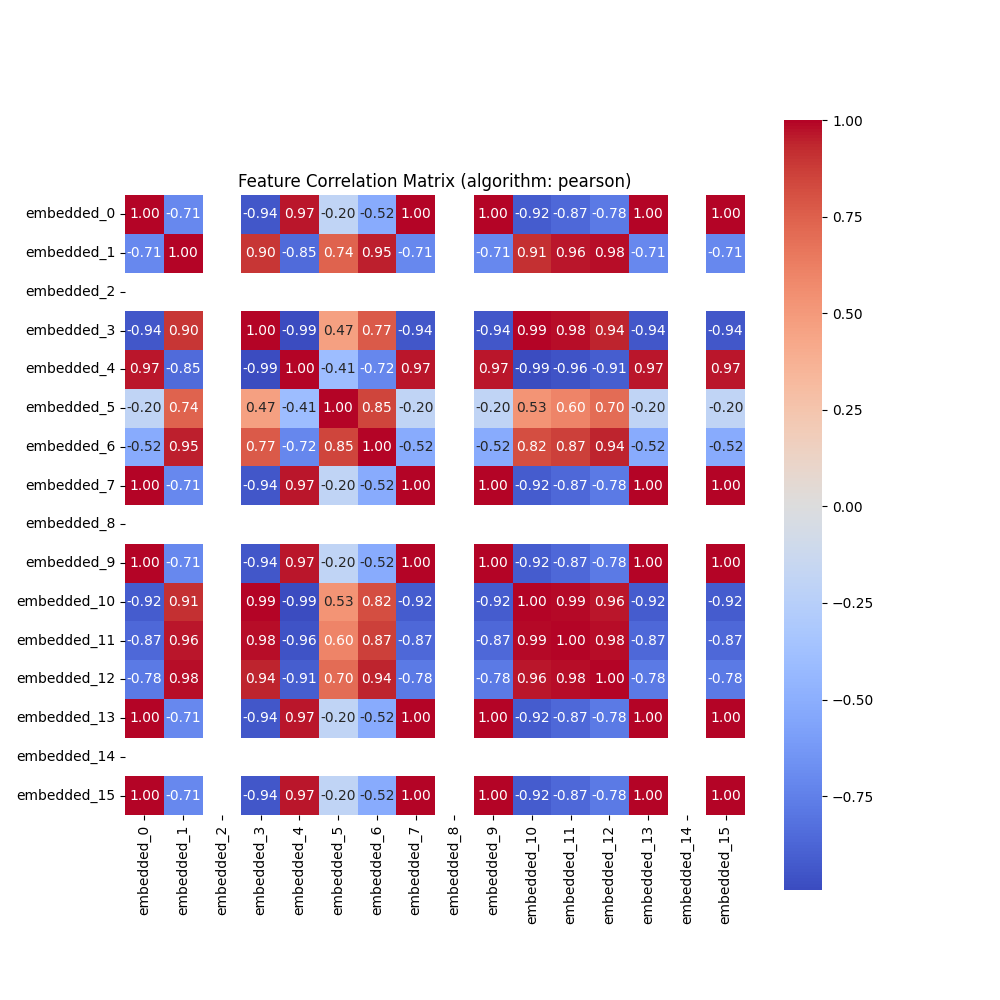
\includegraphics[width=0.8\linewidth]{img/annexes/26_filtered_chunk_extraction_-e_only-max-entropy_-s_none/Transformers 1_correlation_matrix.png}} \\
\hline
\end{longtable}


\begin{longtable}{|c|c|}
\caption{Word2vec 0 Feature Engineering Results on 26\_filtered\_chunk\_extraction\_-e\_only-max-entropy\_-s\_none} \label{tab:26_filtered_chunk_extraction_-e_only-max-entropy_-s_none_word2vec_0_feature_engineering_results}\\
\hline
Dataset Name & 26\_filtered\_chunk\_extraction\_-e\_only-max-entropy\_-s\_none \\ \hline
Instance & Word2vec 0 \\ \hline
\multirow{8}{*}{Best Features} & feature\_1 \\ \cline{2-2}
 & feature\_6 \\ \cline{2-2}
 & feature\_2 \\ \cline{2-2}
 & feature\_3 \\ \cline{2-2}
 & feature\_7 \\ \cline{2-2}
 & feature\_5 \\ \cline{2-2}
 & feature\_0 \\ \cline{2-2}
 & feature\_4 \\ \cline{2-2}
\noalign{\vskip 5mm}
\multicolumn{2}{|c|}{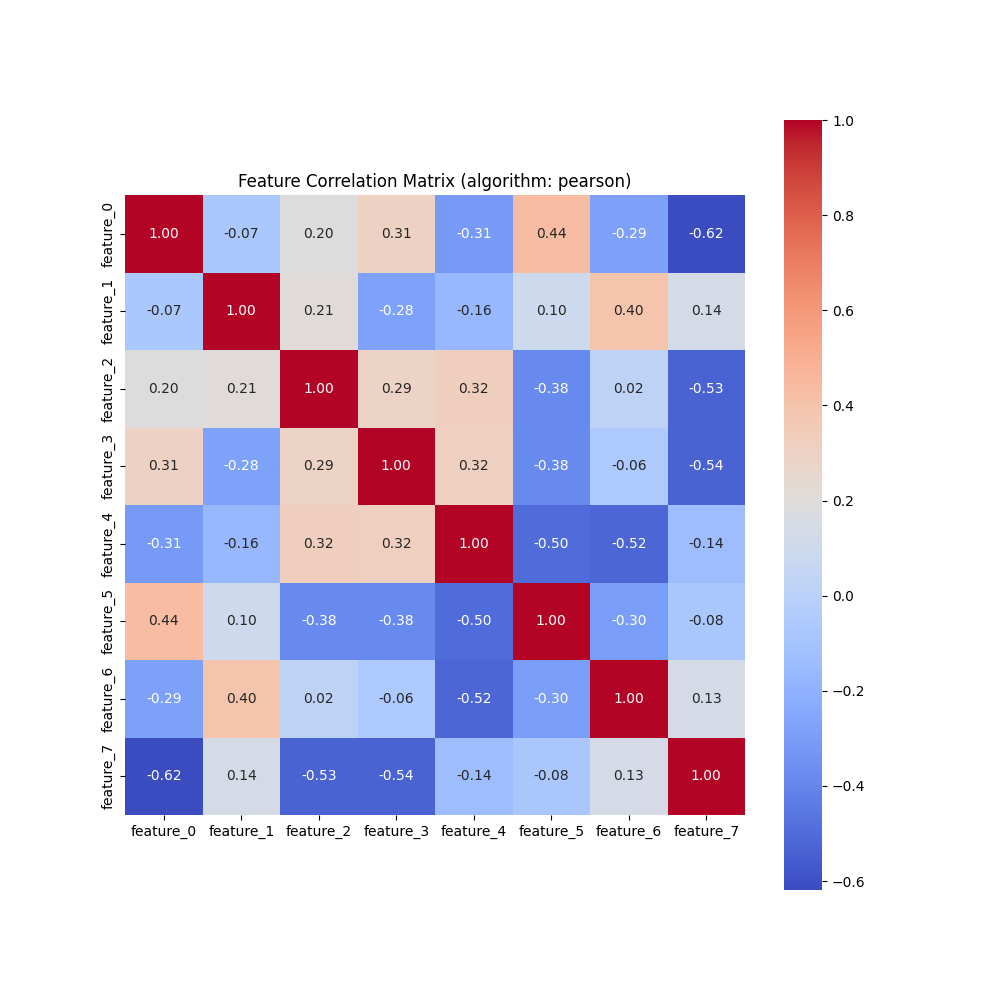
\includegraphics[width=0.8\linewidth]{img/annexes/26_filtered_chunk_extraction_-e_only-max-entropy_-s_none/Word2vec 0_correlation_matrix.png}} \\
\hline
\end{longtable}


\begin{longtable}{|c|c|}
\caption{Word2vec 1 Feature Engineering Results on 26\_filtered\_chunk\_extraction\_-e\_only-max-entropy\_-s\_none} \label{tab:26_filtered_chunk_extraction_-e_only-max-entropy_-s_none_word2vec_1_feature_engineering_results}\\
\hline
Dataset Name & 26\_filtered\_chunk\_extraction\_-e\_only-max-entropy\_-s\_none \\ \hline
Instance & Word2vec 1 \\ \hline
\multirow{8}{*}{Best Features} & feature\_4 \\ \cline{2-2}
 & feature\_7 \\ \cline{2-2}
 & feature\_5 \\ \cline{2-2}
 & feature\_2 \\ \cline{2-2}
 & feature\_3 \\ \cline{2-2}
 & feature\_6 \\ \cline{2-2}
 & feature\_1 \\ \cline{2-2}
 & feature\_0 \\ \cline{2-2}
\noalign{\vskip 5mm}
\multicolumn{2}{|c|}{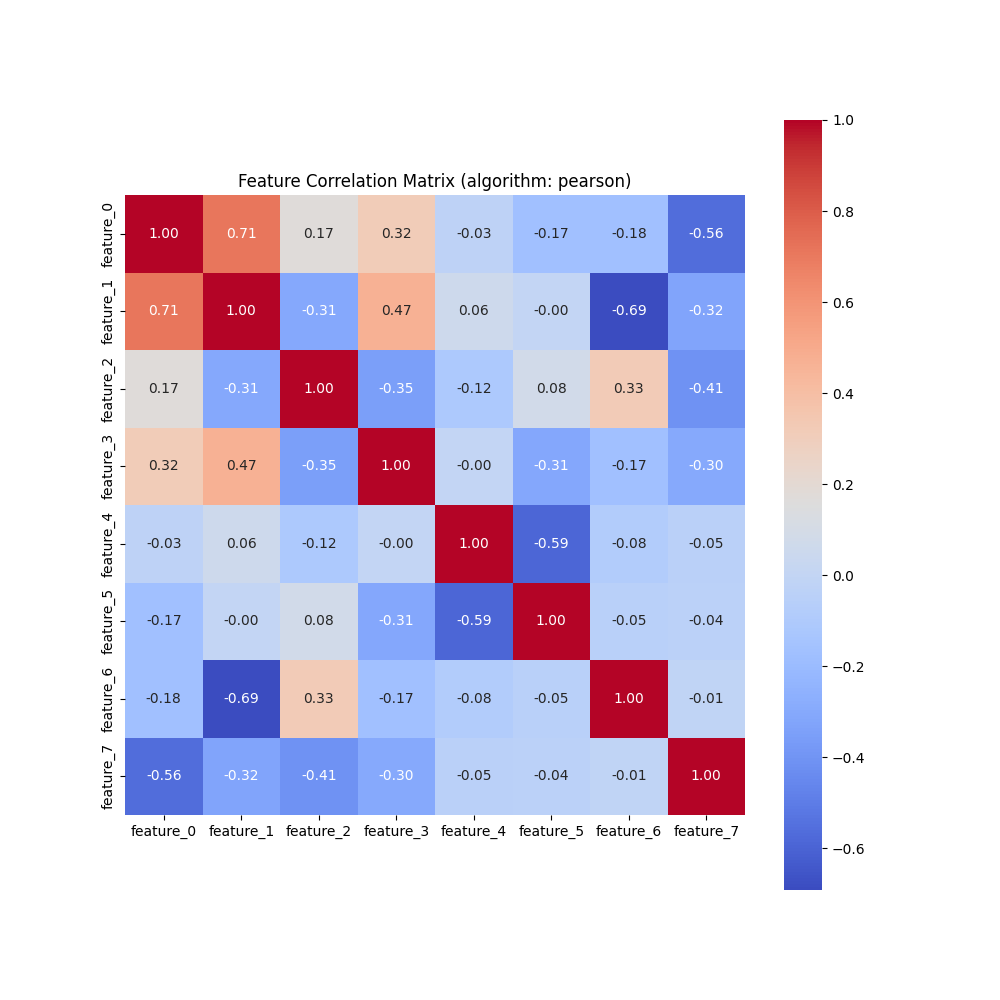
\includegraphics[width=0.8\linewidth]{img/annexes/26_filtered_chunk_extraction_-e_only-max-entropy_-s_none/Word2vec 1_correlation_matrix.png}} \\
\hline
\end{longtable}


\begin{longtable}{|c|c|}
\caption{Word2vec 4 Feature Engineering Results on 26\_filtered\_chunk\_extraction\_-e\_only-max-entropy\_-s\_none} \label{tab:26_filtered_chunk_extraction_-e_only-max-entropy_-s_none_word2vec_4_feature_engineering_results}\\
\hline
Dataset Name & 26\_filtered\_chunk\_extraction\_-e\_only-max-entropy\_-s\_none \\ \hline
Instance & Word2vec 4 \\ \hline
\multirow{8}{*}{Best Features} & feature\_13 \\ \cline{2-2}
 & feature\_9 \\ \cline{2-2}
 & feature\_15 \\ \cline{2-2}
 & feature\_0 \\ \cline{2-2}
 & feature\_6 \\ \cline{2-2}
 & feature\_11 \\ \cline{2-2}
 & feature\_4 \\ \cline{2-2}
 & feature\_10 \\ \cline{2-2}
\noalign{\vskip 5mm}
\multicolumn{2}{|c|}{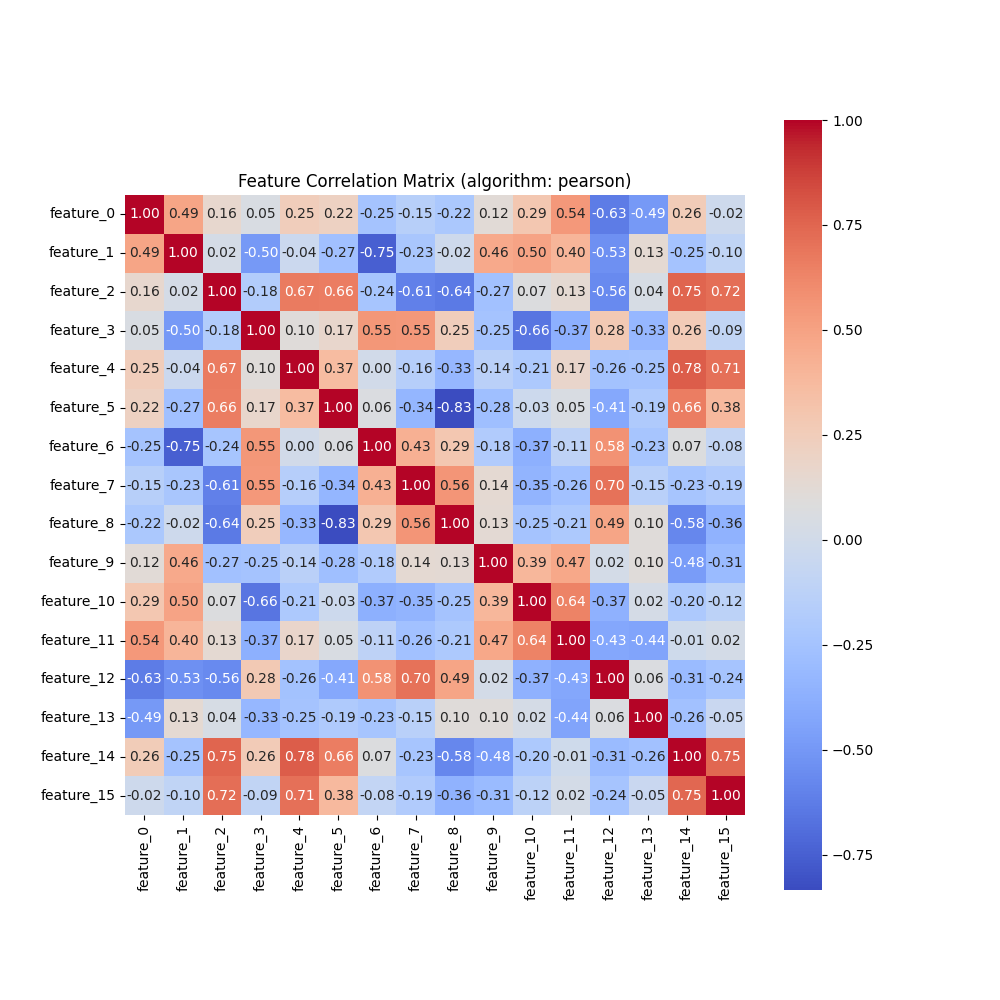
\includegraphics[width=0.8\linewidth]{img/annexes/26_filtered_chunk_extraction_-e_only-max-entropy_-s_none/Word2vec 4_correlation_matrix.png}} \\
\hline
\end{longtable}


\begin{longtable}{|c|c|}
\caption{Word2vec 5 Feature Engineering Results on 26\_filtered\_chunk\_extraction\_-e\_only-max-entropy\_-s\_none} \label{tab:26_filtered_chunk_extraction_-e_only-max-entropy_-s_none_word2vec_5_feature_engineering_results}\\
\hline
Dataset Name & 26\_filtered\_chunk\_extraction\_-e\_only-max-entropy\_-s\_none \\ \hline
Instance & Word2vec 5 \\ \hline
\multirow{8}{*}{Best Features} & feature\_8 \\ \cline{2-2}
 & feature\_14 \\ \cline{2-2}
 & feature\_9 \\ \cline{2-2}
 & feature\_7 \\ \cline{2-2}
 & feature\_10 \\ \cline{2-2}
 & feature\_13 \\ \cline{2-2}
 & feature\_0 \\ \cline{2-2}
 & feature\_6 \\ \cline{2-2}
\noalign{\vskip 5mm}
\multicolumn{2}{|c|}{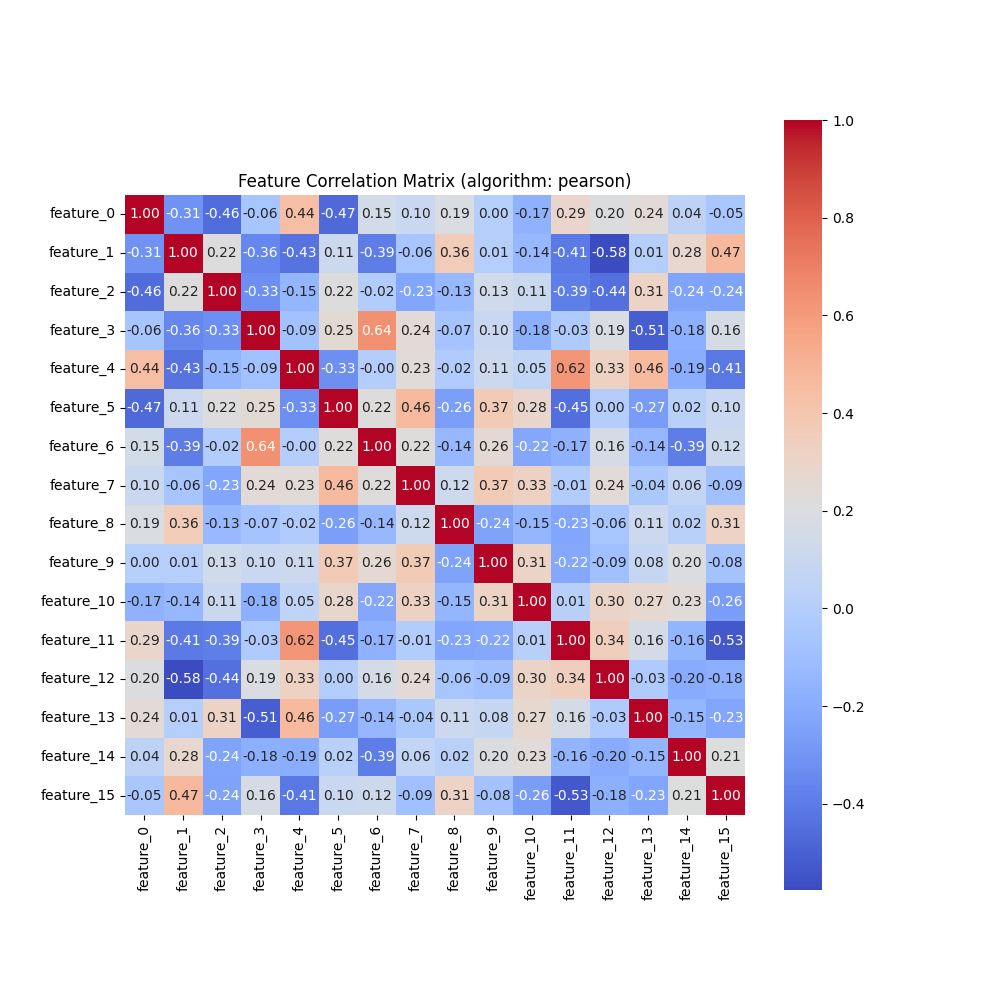
\includegraphics[width=0.8\linewidth]{img/annexes/26_filtered_chunk_extraction_-e_only-max-entropy_-s_none/Word2vec 5_correlation_matrix.png}} \\
\hline
\end{longtable}


\begin{longtable}{|c|c|}
\caption{Word2vec 8 Feature Engineering Results on 26\_filtered\_chunk\_extraction\_-e\_only-max-entropy\_-s\_none} \label{tab:26_filtered_chunk_extraction_-e_only-max-entropy_-s_none_word2vec_8_feature_engineering_results}\\
\hline
Dataset Name & 26\_filtered\_chunk\_extraction\_-e\_only-max-entropy\_-s\_none \\ \hline
Instance & Word2vec 8 \\ \hline
\multirow{8}{*}{Best Features} & feature\_91 \\ \cline{2-2}
 & feature\_75 \\ \cline{2-2}
 & feature\_78 \\ \cline{2-2}
 & feature\_61 \\ \cline{2-2}
 & feature\_83 \\ \cline{2-2}
 & feature\_71 \\ \cline{2-2}
 & feature\_22 \\ \cline{2-2}
 & feature\_33 \\ \cline{2-2}
\noalign{\vskip 5mm}
\multicolumn{2}{|c|}{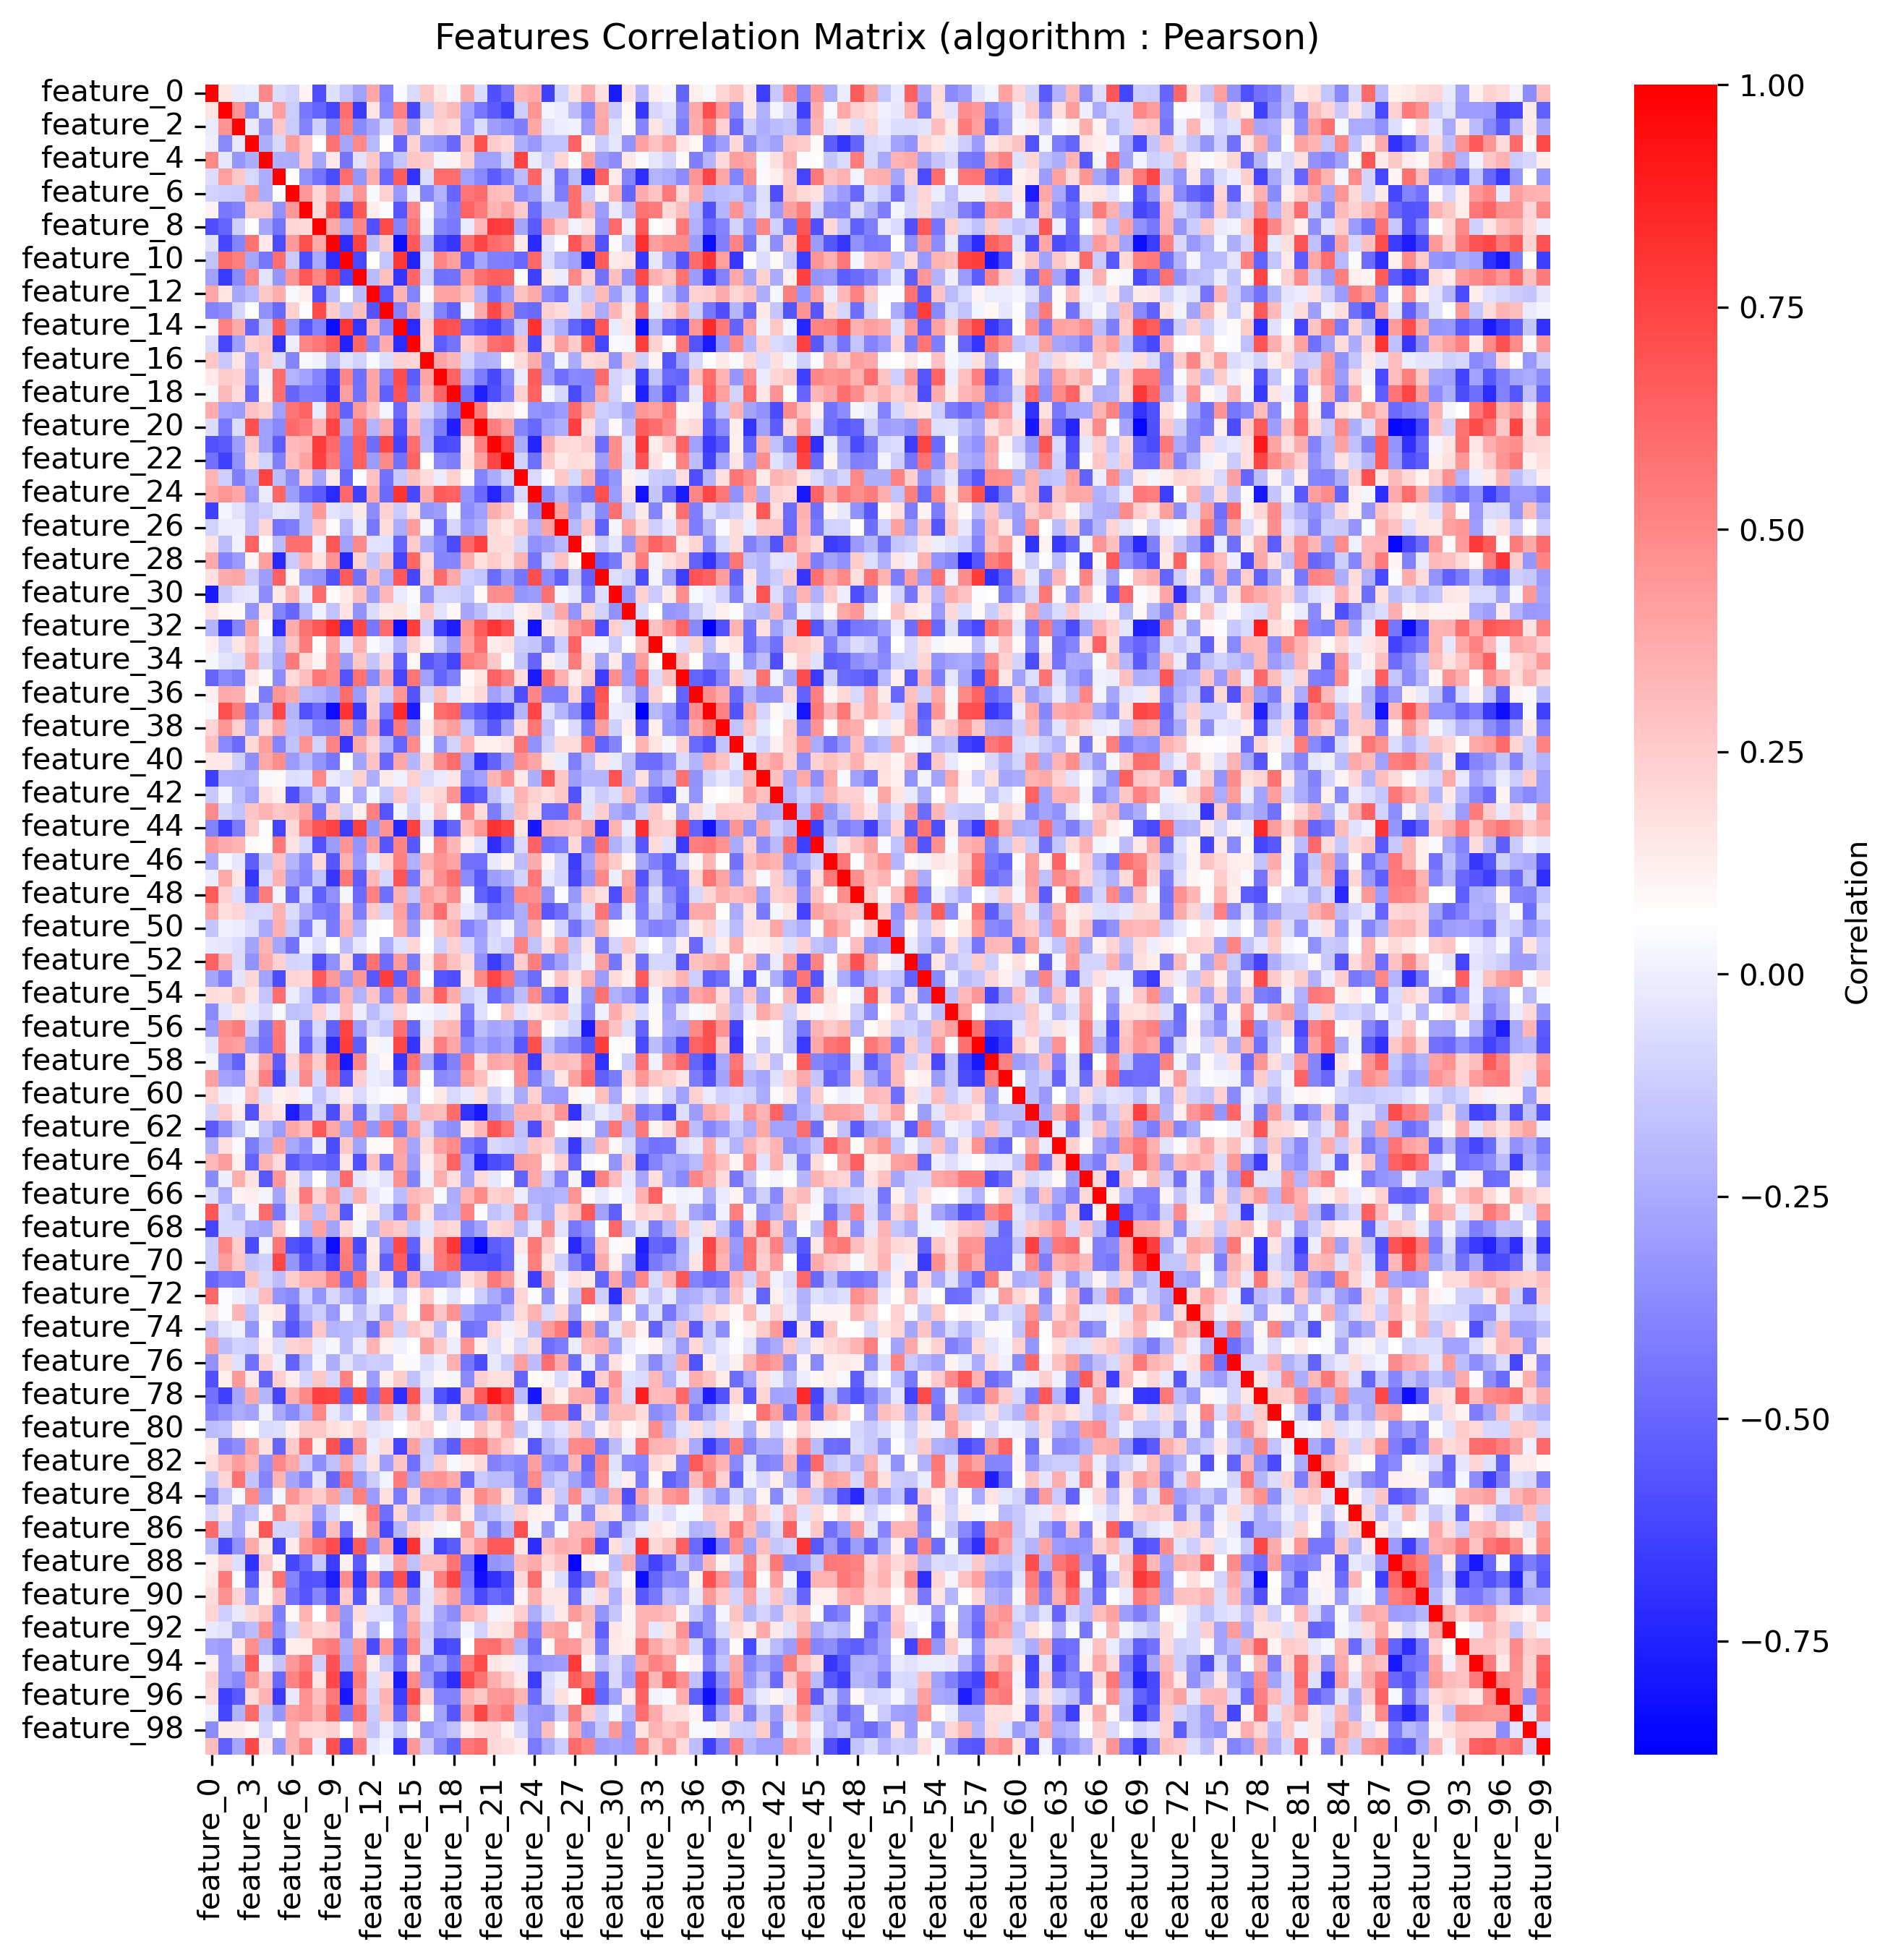
\includegraphics[width=0.8\linewidth]{img/annexes/26_filtered_chunk_extraction_-e_only-max-entropy_-s_none/Word2vec 8_correlation_matrix.png}} \\
\hline
\end{longtable}


\begin{longtable}{|c|c|}
\caption{Word2vec 9 Feature Engineering Results on 26\_filtered\_chunk\_extraction\_-e\_only-max-entropy\_-s\_none} \label{tab:26_filtered_chunk_extraction_-e_only-max-entropy_-s_none_word2vec_9_feature_engineering_results}\\
\hline
Dataset Name & 26\_filtered\_chunk\_extraction\_-e\_only-max-entropy\_-s\_none \\ \hline
Instance & Word2vec 9 \\ \hline
\multirow{8}{*}{Best Features} & feature\_73 \\ \cline{2-2}
 & feature\_18 \\ \cline{2-2}
 & feature\_14 \\ \cline{2-2}
 & feature\_32 \\ \cline{2-2}
 & feature\_99 \\ \cline{2-2}
 & feature\_7 \\ \cline{2-2}
 & feature\_94 \\ \cline{2-2}
 & feature\_19 \\ \cline{2-2}
\noalign{\vskip 5mm}
\multicolumn{2}{|c|}{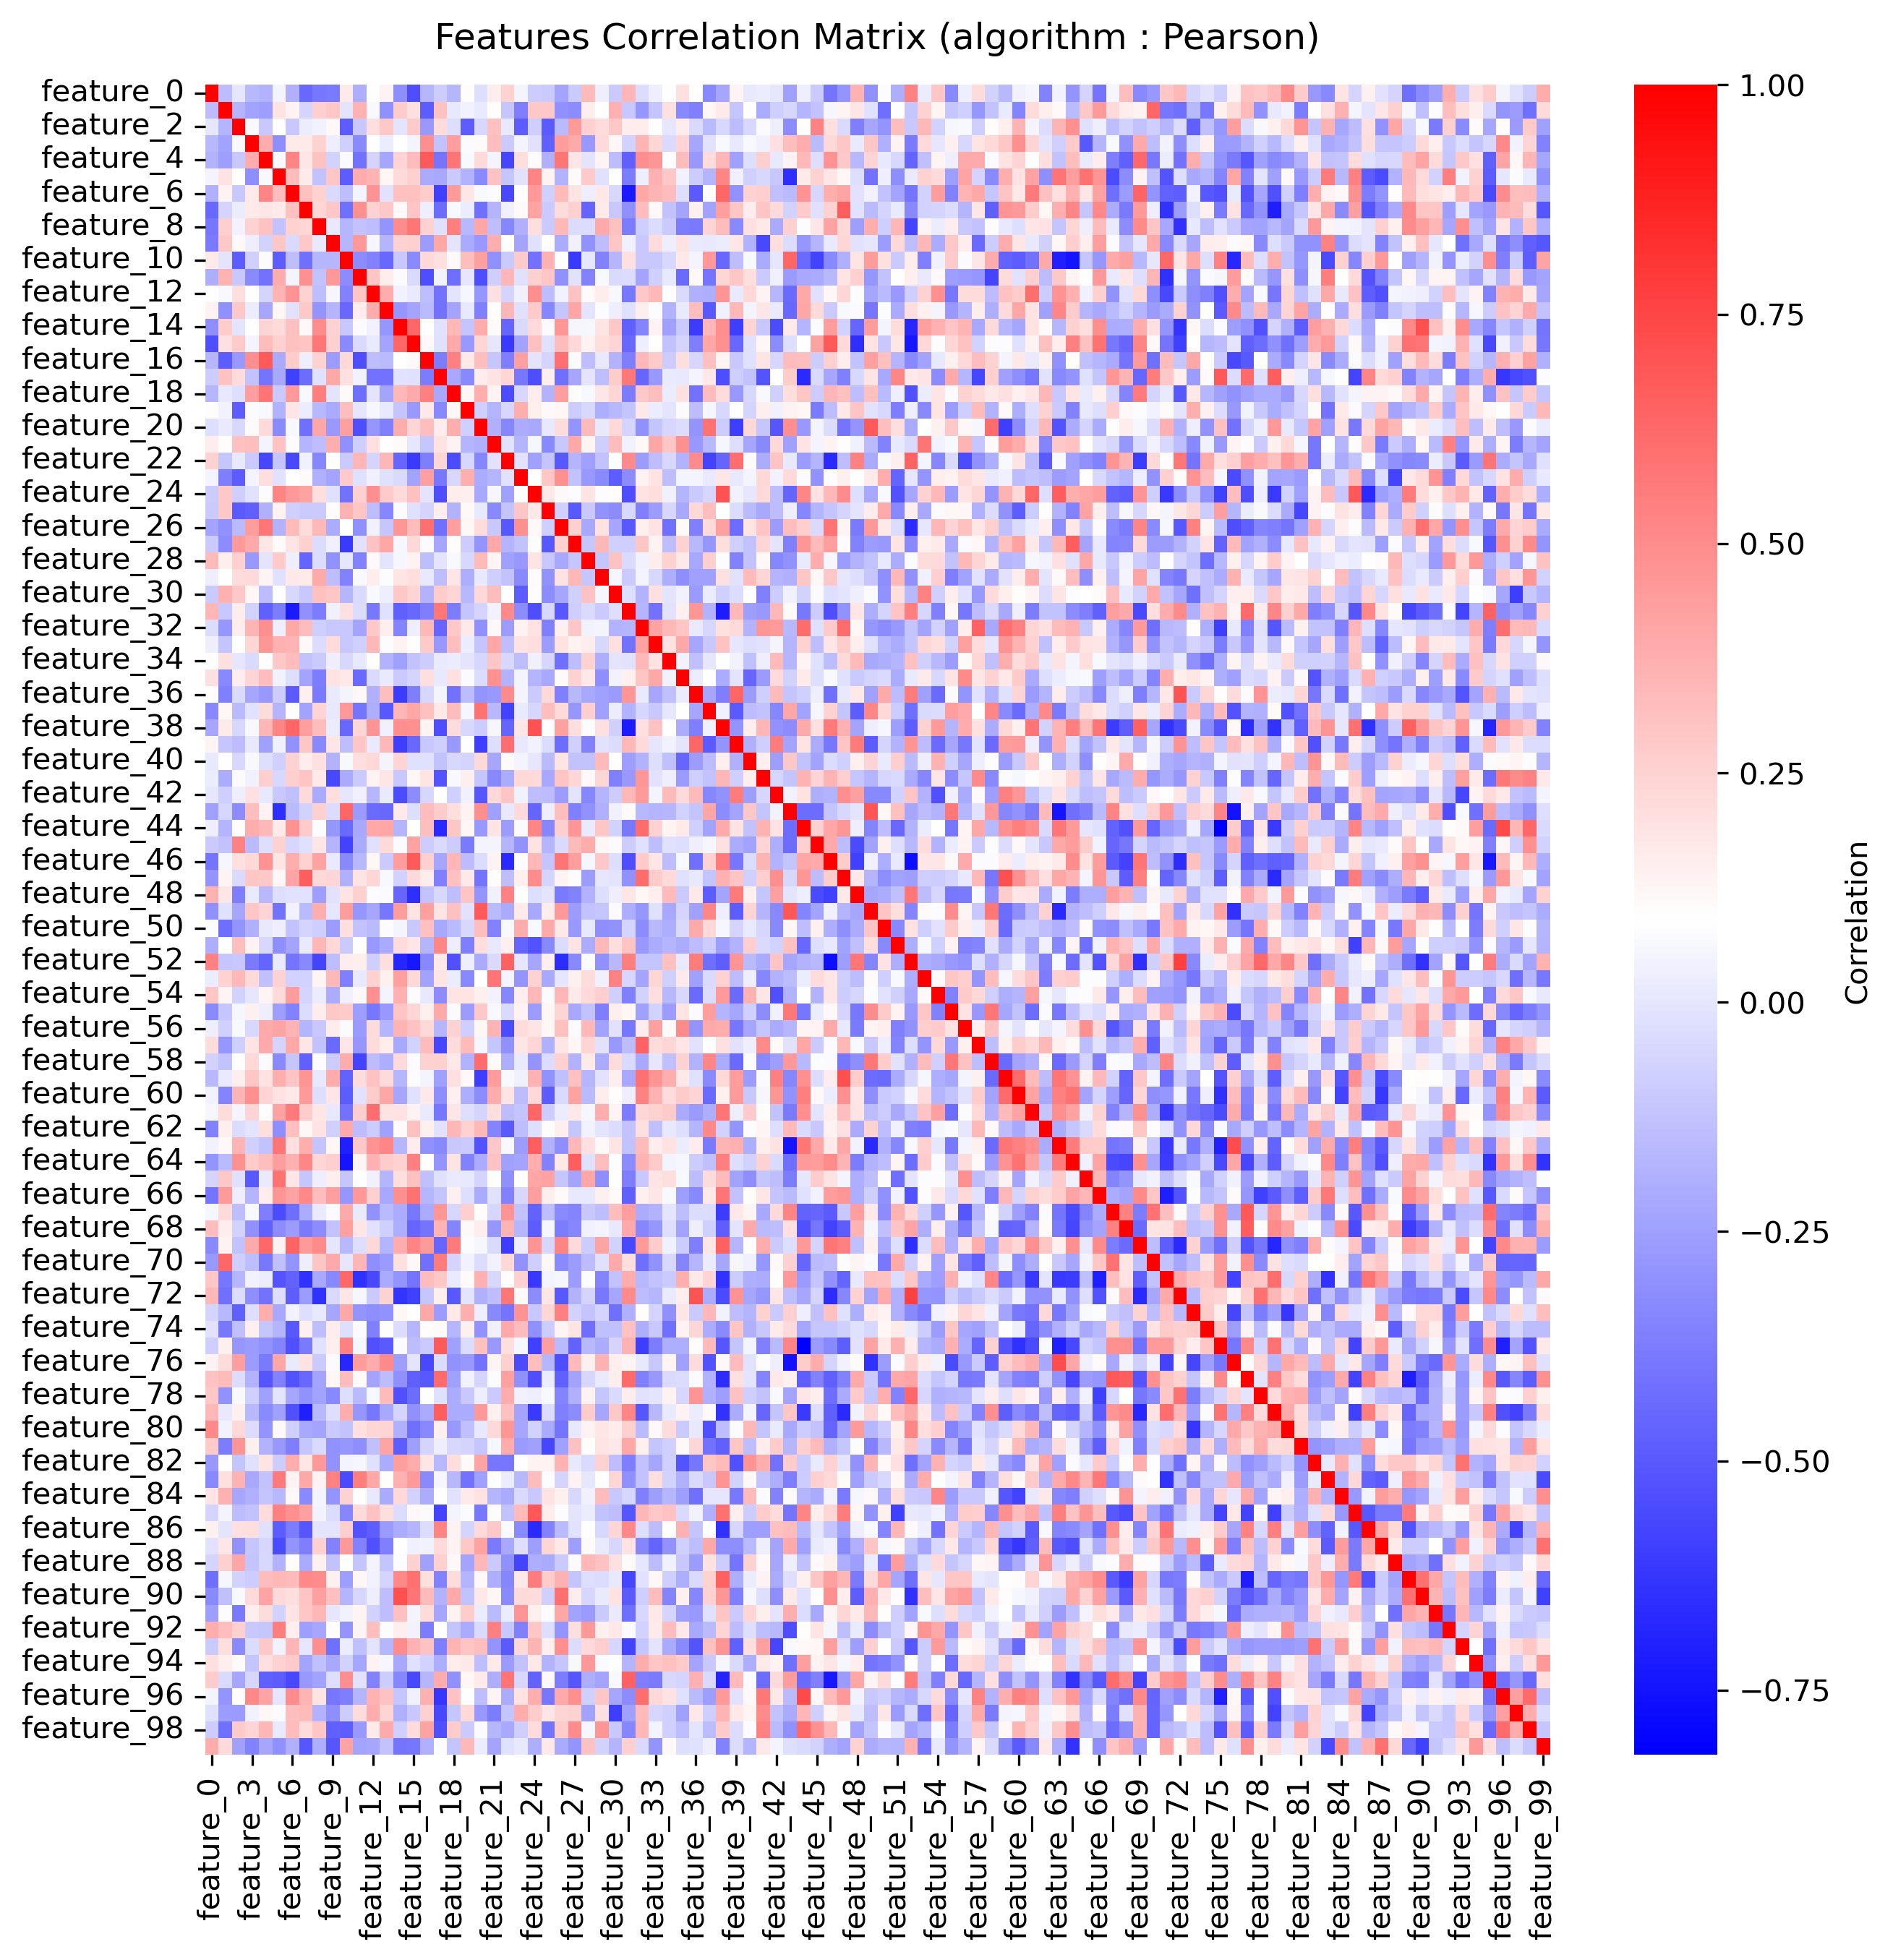
\includegraphics[width=0.8\linewidth]{img/annexes/26_filtered_chunk_extraction_-e_only-max-entropy_-s_none/Word2vec 9_correlation_matrix.png}} \\
\hline
\end{longtable}


\subsection{27\_filtered\_chunk\_extraction\_-e\_only-max-entropy\_-s\_activate}

\begin{longtable}{|c|c|}
\caption{Transformers 0 Feature Engineering Results on 27\_filtered\_chunk\_extraction\_-e\_only-max-entropy\_-s\_activate} \label{tab:27_filtered_chunk_extraction_-e_only-max-entropy_-s_activate_transformers_0_feature_engineering_results}\\
\hline
Dataset Name & 27\_filtered\_chunk\_extraction\_-e\_only-max-entropy\_-s\_activate \\ \hline
Instance & Transformers 0 \\ \hline
\multirow{8}{*}{Best Features} & embedded\_0 \\ \cline{2-2}
 & embedded\_1 \\ \cline{2-2}
 & embedded\_4 \\ \cline{2-2}
 & embedded\_5 \\ \cline{2-2}
 & embedded\_7 \\ \cline{2-2}
 & embedded\_6 \\ \cline{2-2}
 & embedded\_3 \\ \cline{2-2}
 & embedded\_2 \\ \cline{2-2}
\noalign{\vskip 5mm}
\multicolumn{2}{|c|}{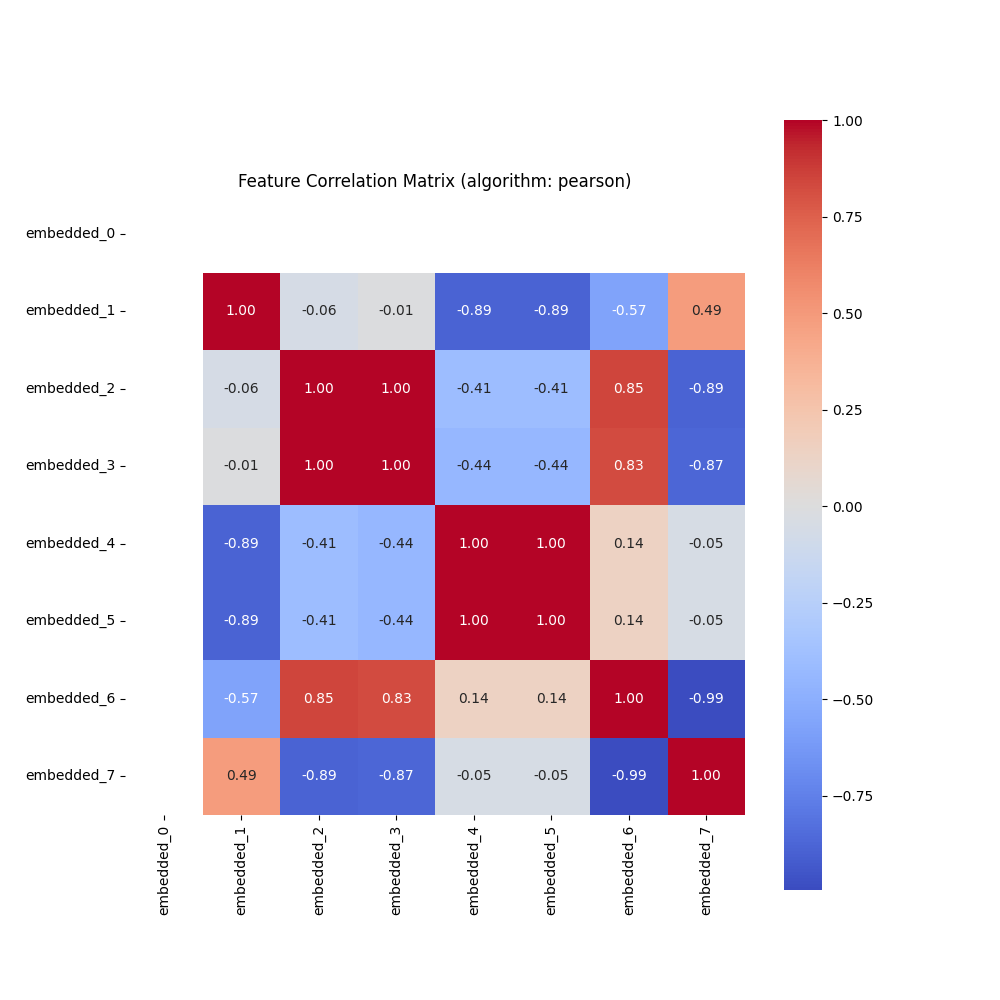
\includegraphics[width=0.8\linewidth]{img/annexes/27_filtered_chunk_extraction_-e_only-max-entropy_-s_activate/Transformers 0_correlation_matrix.png}} \\
\hline
\end{longtable}


\begin{longtable}{|c|c|}
\caption{Transformers 1 Feature Engineering Results on 27\_filtered\_chunk\_extraction\_-e\_only-max-entropy\_-s\_activate} \label{tab:27_filtered_chunk_extraction_-e_only-max-entropy_-s_activate_transformers_1_feature_engineering_results}\\
\hline
Dataset Name & 27\_filtered\_chunk\_extraction\_-e\_only-max-entropy\_-s\_activate \\ \hline
Instance & Transformers 1 \\ \hline
\multirow{8}{*}{Best Features} & embedded\_0 \\ \cline{2-2}
 & embedded\_6 \\ \cline{2-2}
 & embedded\_7 \\ \cline{2-2}
 & embedded\_9 \\ \cline{2-2}
 & embedded\_8 \\ \cline{2-2}
 & embedded\_10 \\ \cline{2-2}
 & embedded\_5 \\ \cline{2-2}
 & embedded\_3 \\ \cline{2-2}
\noalign{\vskip 5mm}
\multicolumn{2}{|c|}{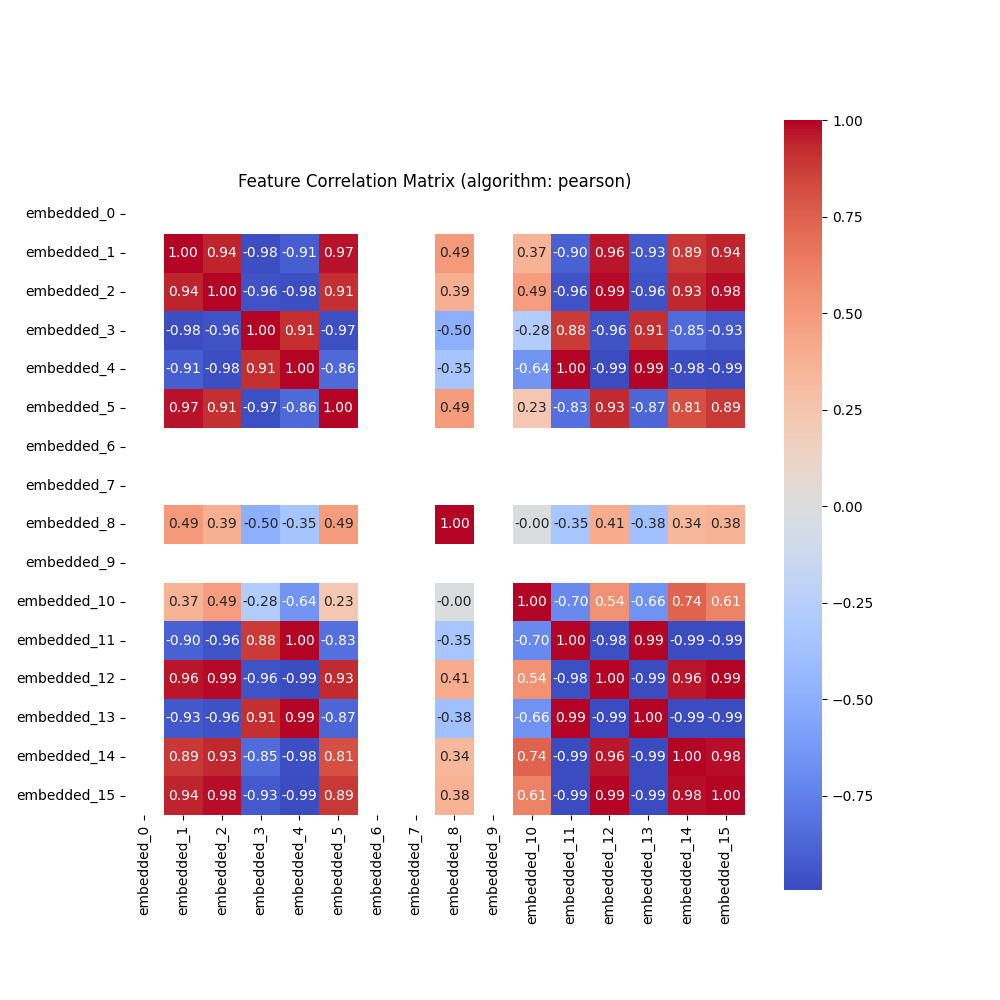
\includegraphics[width=0.8\linewidth]{img/annexes/27_filtered_chunk_extraction_-e_only-max-entropy_-s_activate/Transformers 1_correlation_matrix.png}} \\
\hline
\end{longtable}


\begin{longtable}{|c|c|}
\caption{Transformers 2 Feature Engineering Results on 27\_filtered\_chunk\_extraction\_-e\_only-max-entropy\_-s\_activate} \label{tab:27_filtered_chunk_extraction_-e_only-max-entropy_-s_activate_transformers_2_feature_engineering_results}\\
\hline
Dataset Name & 27\_filtered\_chunk\_extraction\_-e\_only-max-entropy\_-s\_activate \\ \hline
Instance & Transformers 2 \\ \hline
\multirow{8}{*}{Best Features} & embedded\_0 \\ \cline{2-2}
 & embedded\_3 \\ \cline{2-2}
 & embedded\_7 \\ \cline{2-2}
 & embedded\_6 \\ \cline{2-2}
 & embedded\_1 \\ \cline{2-2}
 & embedded\_2 \\ \cline{2-2}
 & embedded\_5 \\ \cline{2-2}
 & embedded\_4 \\ \cline{2-2}
\noalign{\vskip 5mm}
\multicolumn{2}{|c|}{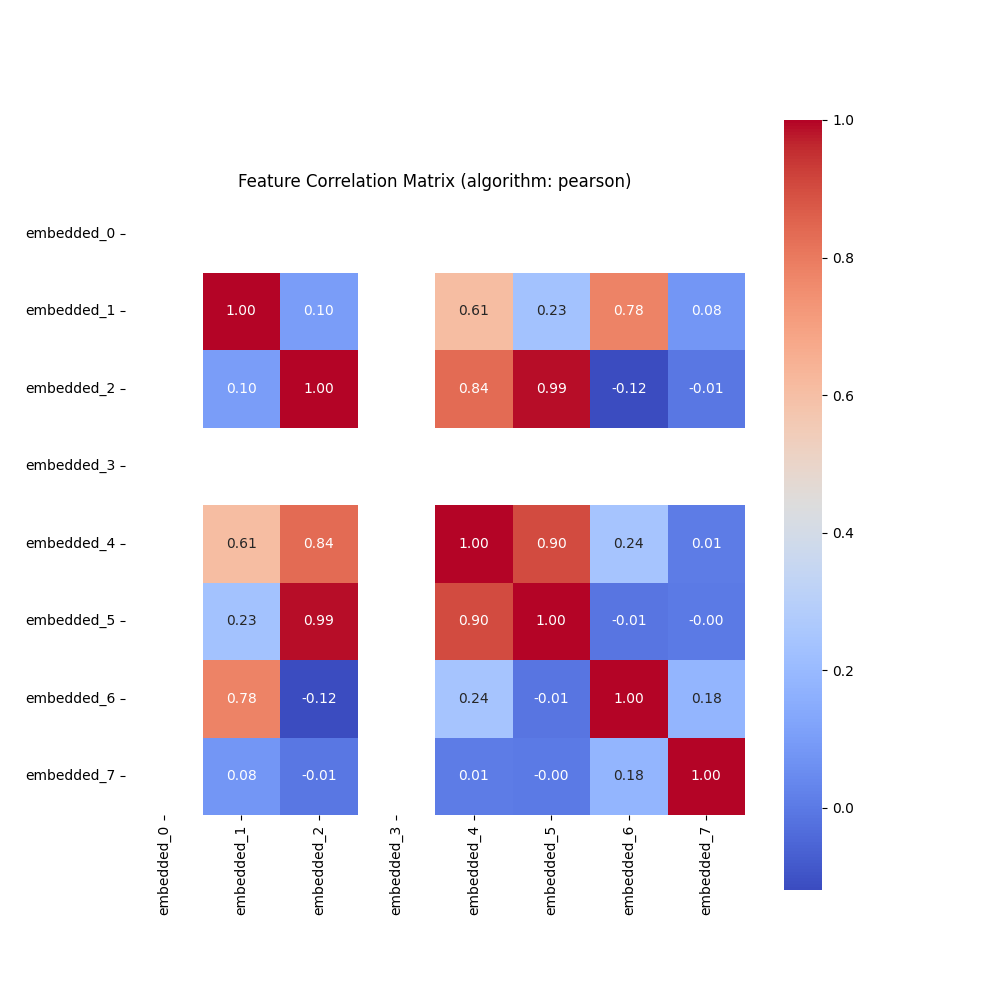
\includegraphics[width=0.8\linewidth]{img/annexes/27_filtered_chunk_extraction_-e_only-max-entropy_-s_activate/Transformers 2_correlation_matrix.png}} \\
\hline
\end{longtable}


\begin{longtable}{|c|c|}
\caption{Transformers 3 Feature Engineering Results on 27\_filtered\_chunk\_extraction\_-e\_only-max-entropy\_-s\_activate} \label{tab:27_filtered_chunk_extraction_-e_only-max-entropy_-s_activate_transformers_3_feature_engineering_results}\\
\hline
Dataset Name & 27\_filtered\_chunk\_extraction\_-e\_only-max-entropy\_-s\_activate \\ \hline
Instance & Transformers 3 \\ \hline
\multirow{8}{*}{Best Features} & embedded\_0 \\ \cline{2-2}
 & embedded\_2 \\ \cline{2-2}
 & embedded\_3 \\ \cline{2-2}
 & embedded\_7 \\ \cline{2-2}
 & embedded\_14 \\ \cline{2-2}
 & embedded\_9 \\ \cline{2-2}
 & embedded\_13 \\ \cline{2-2}
 & embedded\_5 \\ \cline{2-2}
\noalign{\vskip 5mm}
\multicolumn{2}{|c|}{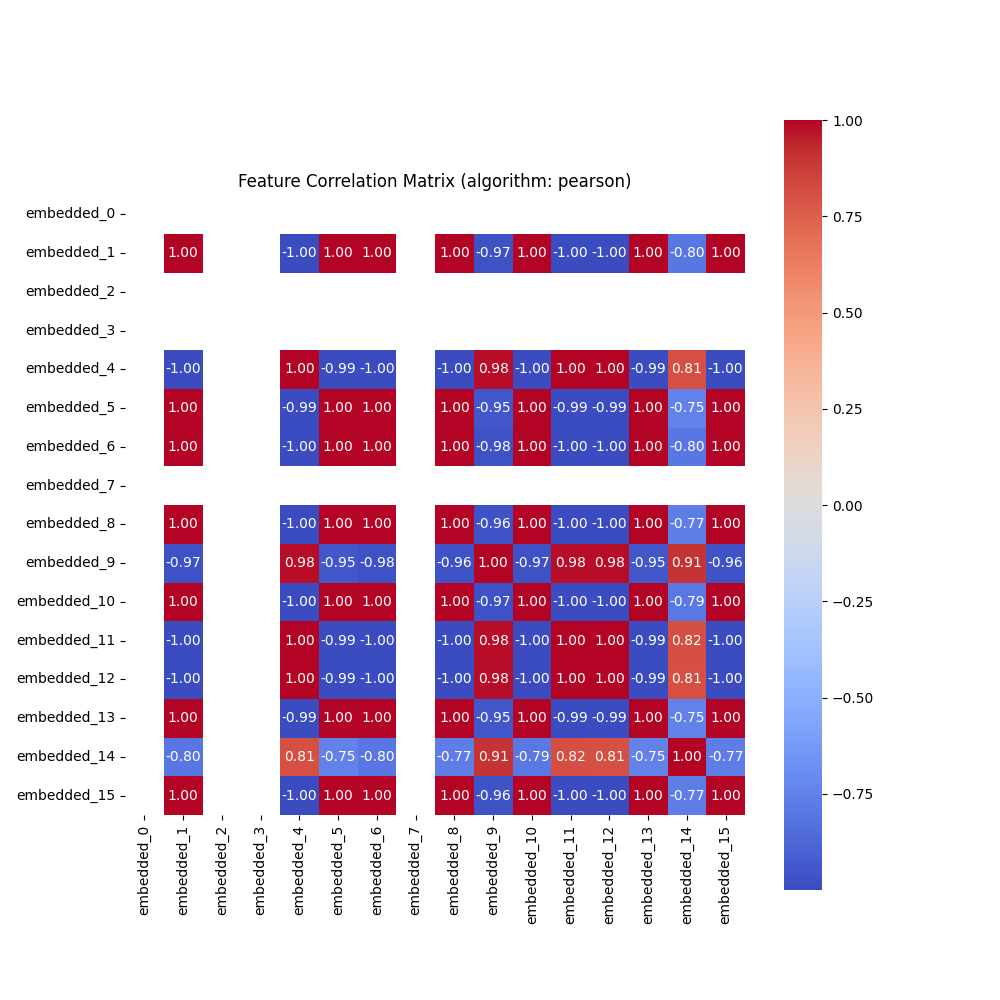
\includegraphics[width=0.8\linewidth]{img/annexes/27_filtered_chunk_extraction_-e_only-max-entropy_-s_activate/Transformers 3_correlation_matrix.png}} \\
\hline
\end{longtable}


\begin{longtable}{|c|c|}
\caption{Transformers 4 Feature Engineering Results on 27\_filtered\_chunk\_extraction\_-e\_only-max-entropy\_-s\_activate} \label{tab:27_filtered_chunk_extraction_-e_only-max-entropy_-s_activate_transformers_4_feature_engineering_results}\\
\hline
Dataset Name & 27\_filtered\_chunk\_extraction\_-e\_only-max-entropy\_-s\_activate \\ \hline
Instance & Transformers 4 \\ \hline
\multirow{8}{*}{Best Features} & embedded\_4 \\ \cline{2-2}
 & embedded\_1 \\ \cline{2-2}
 & embedded\_5 \\ \cline{2-2}
 & embedded\_7 \\ \cline{2-2}
 & embedded\_6 \\ \cline{2-2}
 & embedded\_3 \\ \cline{2-2}
 & embedded\_0 \\ \cline{2-2}
 & embedded\_2 \\ \cline{2-2}
\noalign{\vskip 5mm}
\multicolumn{2}{|c|}{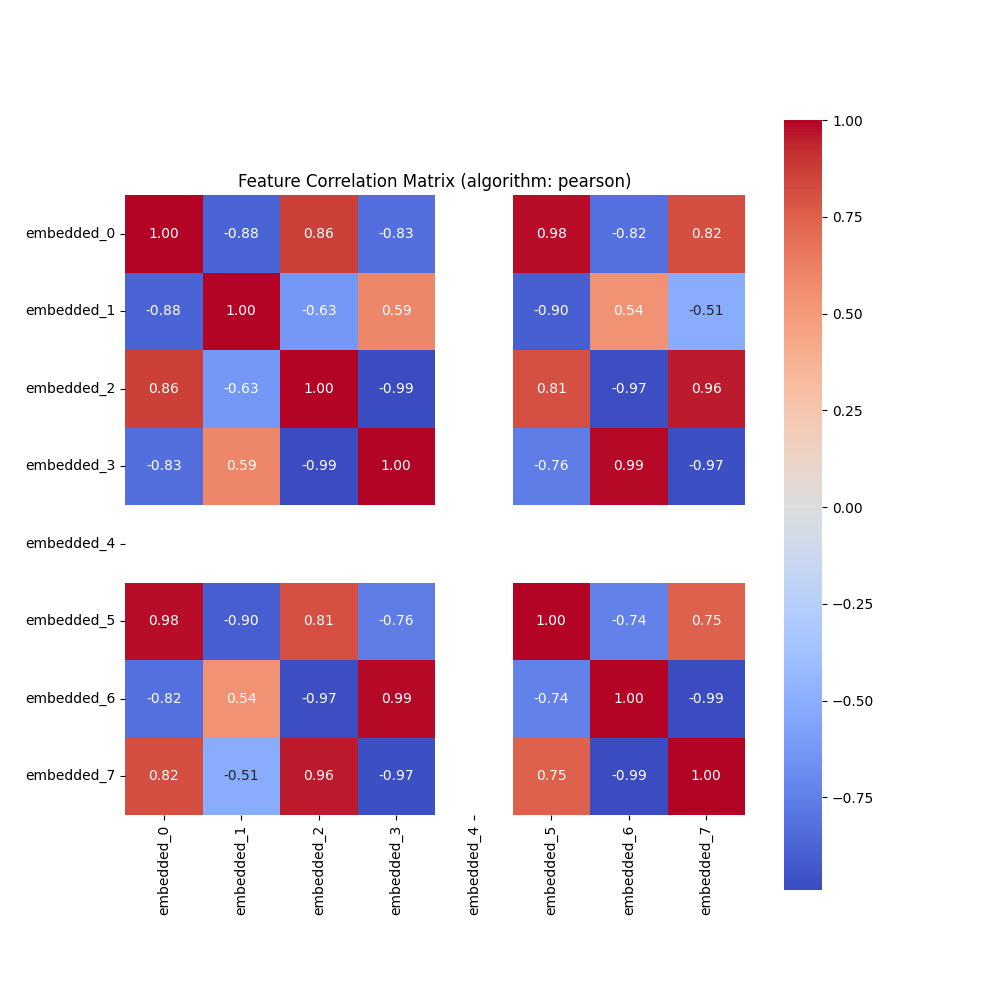
\includegraphics[width=0.8\linewidth]{img/annexes/27_filtered_chunk_extraction_-e_only-max-entropy_-s_activate/Transformers 4_correlation_matrix.png}} \\
\hline
\end{longtable}


\begin{longtable}{|c|c|}
\caption{Transformers 5 Feature Engineering Results on 27\_filtered\_chunk\_extraction\_-e\_only-max-entropy\_-s\_activate} \label{tab:27_filtered_chunk_extraction_-e_only-max-entropy_-s_activate_transformers_5_feature_engineering_results}\\
\hline
Dataset Name & 27\_filtered\_chunk\_extraction\_-e\_only-max-entropy\_-s\_activate \\ \hline
Instance & Transformers 5 \\ \hline
\multirow{8}{*}{Best Features} & embedded\_2 \\ \cline{2-2}
 & embedded\_4 \\ \cline{2-2}
 & embedded\_5 \\ \cline{2-2}
 & embedded\_6 \\ \cline{2-2}
 & embedded\_8 \\ \cline{2-2}
 & embedded\_14 \\ \cline{2-2}
 & embedded\_15 \\ \cline{2-2}
 & embedded\_0 \\ \cline{2-2}
\noalign{\vskip 5mm}
\multicolumn{2}{|c|}{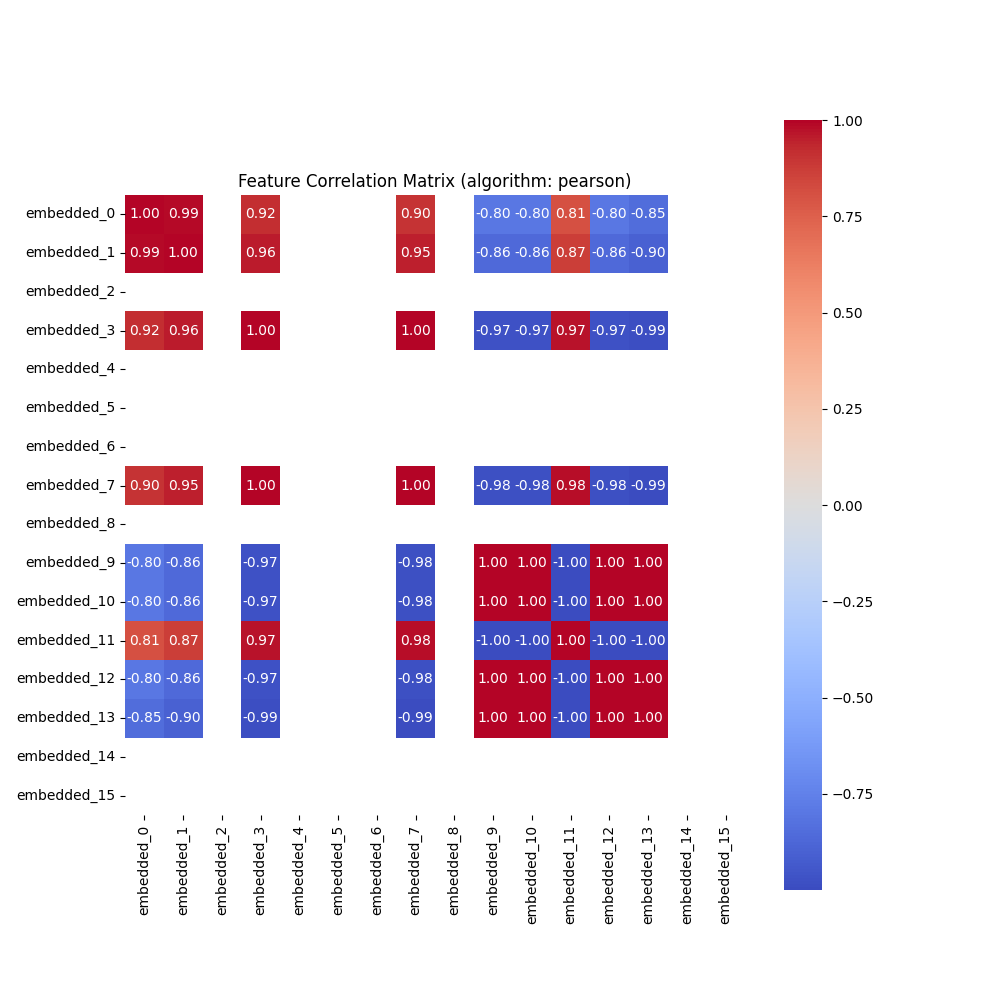
\includegraphics[width=0.8\linewidth]{img/annexes/27_filtered_chunk_extraction_-e_only-max-entropy_-s_activate/Transformers 5_correlation_matrix.png}} \\
\hline
\end{longtable}


\begin{longtable}{|c|c|}
\caption{Transformers 6 Feature Engineering Results on 27\_filtered\_chunk\_extraction\_-e\_only-max-entropy\_-s\_activate} \label{tab:27_filtered_chunk_extraction_-e_only-max-entropy_-s_activate_transformers_6_feature_engineering_results}\\
\hline
Dataset Name & 27\_filtered\_chunk\_extraction\_-e\_only-max-entropy\_-s\_activate \\ \hline
Instance & Transformers 6 \\ \hline
\multirow{8}{*}{Best Features} & embedded\_2 \\ \cline{2-2}
 & embedded\_3 \\ \cline{2-2}
 & embedded\_0 \\ \cline{2-2}
 & embedded\_5 \\ \cline{2-2}
 & embedded\_6 \\ \cline{2-2}
 & embedded\_1 \\ \cline{2-2}
 & embedded\_7 \\ \cline{2-2}
 & embedded\_4 \\ \cline{2-2}
\noalign{\vskip 5mm}
\multicolumn{2}{|c|}{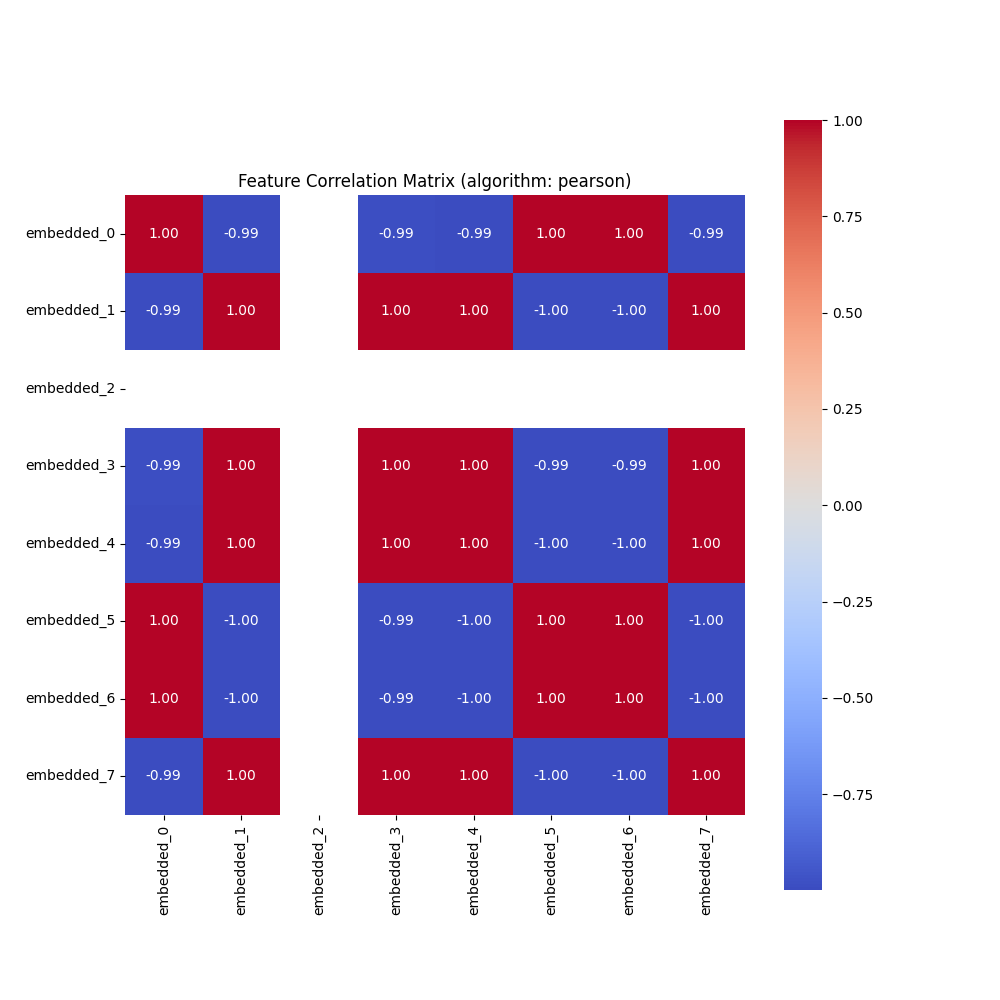
\includegraphics[width=0.8\linewidth]{img/annexes/27_filtered_chunk_extraction_-e_only-max-entropy_-s_activate/Transformers 6_correlation_matrix.png}} \\
\hline
\end{longtable}


\begin{longtable}{|c|c|}
\caption{Transformers 7 Feature Engineering Results on 27\_filtered\_chunk\_extraction\_-e\_only-max-entropy\_-s\_activate} \label{tab:27_filtered_chunk_extraction_-e_only-max-entropy_-s_activate_transformers_7_feature_engineering_results}\\
\hline
Dataset Name & 27\_filtered\_chunk\_extraction\_-e\_only-max-entropy\_-s\_activate \\ \hline
Instance & Transformers 7 \\ \hline
\multirow{8}{*}{Best Features} & embedded\_5 \\ \cline{2-2}
 & embedded\_11 \\ \cline{2-2}
 & embedded\_12 \\ \cline{2-2}
 & embedded\_13 \\ \cline{2-2}
 & embedded\_14 \\ \cline{2-2}
 & embedded\_15 \\ \cline{2-2}
 & embedded\_3 \\ \cline{2-2}
 & embedded\_4 \\ \cline{2-2}
\noalign{\vskip 5mm}
\multicolumn{2}{|c|}{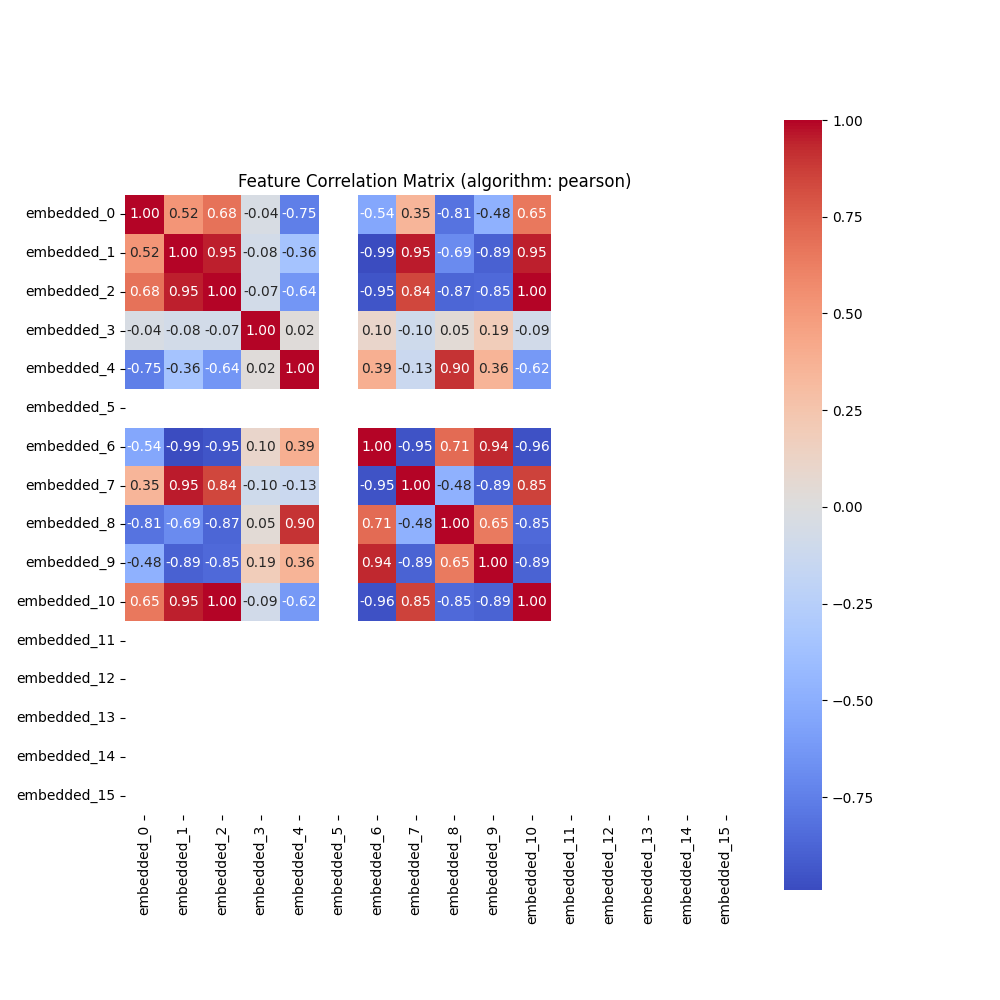
\includegraphics[width=0.8\linewidth]{img/annexes/27_filtered_chunk_extraction_-e_only-max-entropy_-s_activate/Transformers 7_correlation_matrix.png}} \\
\hline
\end{longtable}


\begin{longtable}{|c|c|}
\caption{Word2vec 0 Feature Engineering Results on 27\_filtered\_chunk\_extraction\_-e\_only-max-entropy\_-s\_activate} \label{tab:27_filtered_chunk_extraction_-e_only-max-entropy_-s_activate_word2vec_0_feature_engineering_results}\\
\hline
Dataset Name & 27\_filtered\_chunk\_extraction\_-e\_only-max-entropy\_-s\_activate \\ \hline
Instance & Word2vec 0 \\ \hline
\multirow{8}{*}{Best Features} & feature\_5 \\ \cline{2-2}
 & feature\_7 \\ \cline{2-2}
 & feature\_1 \\ \cline{2-2}
 & feature\_6 \\ \cline{2-2}
 & feature\_4 \\ \cline{2-2}
 & feature\_3 \\ \cline{2-2}
 & feature\_2 \\ \cline{2-2}
 & feature\_0 \\ \cline{2-2}
\noalign{\vskip 5mm}
\multicolumn{2}{|c|}{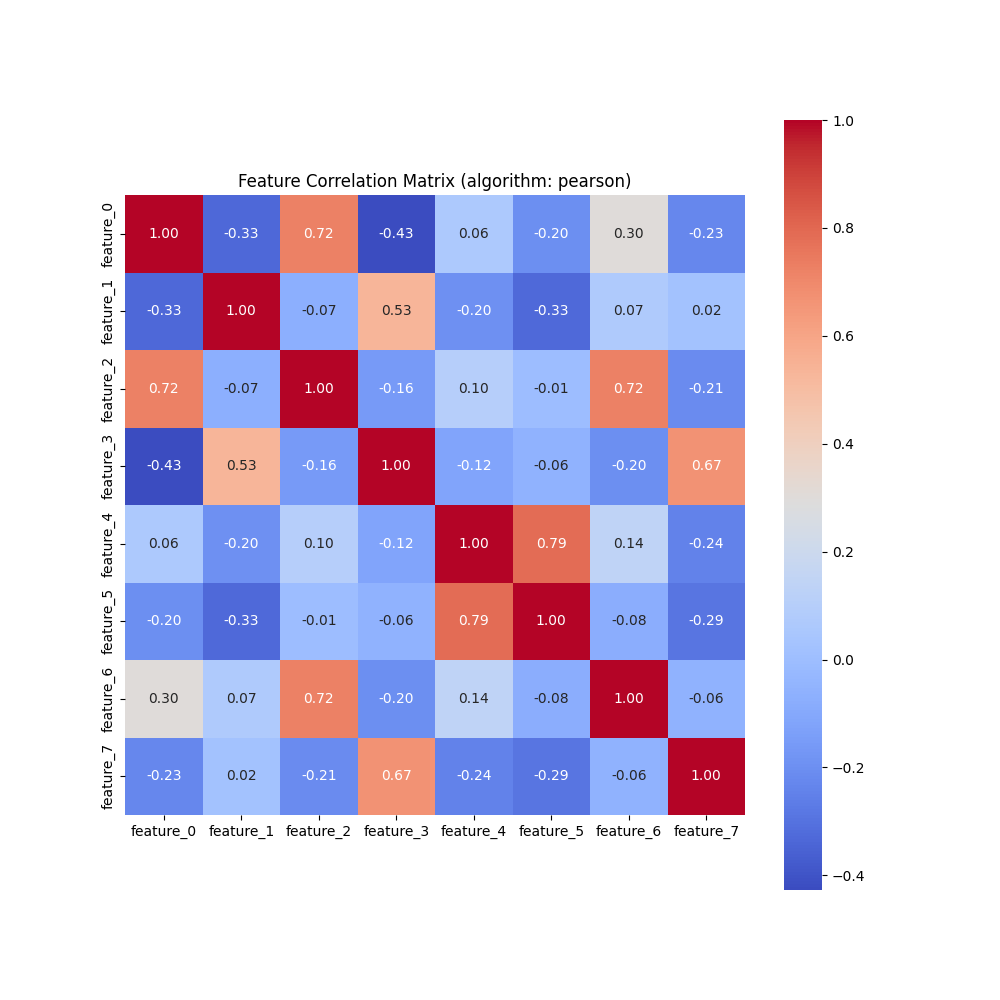
\includegraphics[width=0.8\linewidth]{img/annexes/27_filtered_chunk_extraction_-e_only-max-entropy_-s_activate/Word2vec 0_correlation_matrix.png}} \\
\hline
\end{longtable}


\begin{longtable}{|c|c|}
\caption{Word2vec 1 Feature Engineering Results on 27\_filtered\_chunk\_extraction\_-e\_only-max-entropy\_-s\_activate} \label{tab:27_filtered_chunk_extraction_-e_only-max-entropy_-s_activate_word2vec_1_feature_engineering_results}\\
\hline
Dataset Name & 27\_filtered\_chunk\_extraction\_-e\_only-max-entropy\_-s\_activate \\ \hline
Instance & Word2vec 1 \\ \hline
\multirow{8}{*}{Best Features} & feature\_1 \\ \cline{2-2}
 & feature\_4 \\ \cline{2-2}
 & feature\_5 \\ \cline{2-2}
 & feature\_0 \\ \cline{2-2}
 & feature\_2 \\ \cline{2-2}
 & feature\_7 \\ \cline{2-2}
 & feature\_6 \\ \cline{2-2}
 & feature\_3 \\ \cline{2-2}
\noalign{\vskip 5mm}
\multicolumn{2}{|c|}{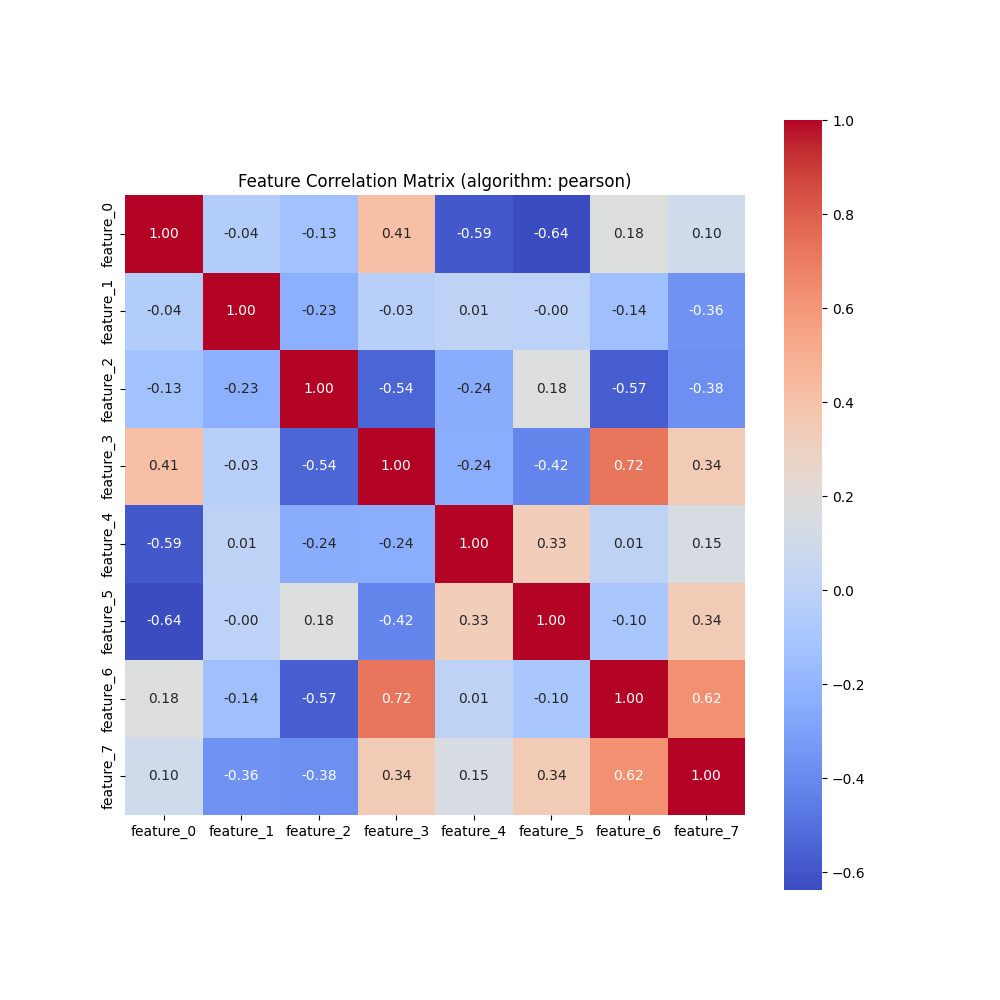
\includegraphics[width=0.8\linewidth]{img/annexes/27_filtered_chunk_extraction_-e_only-max-entropy_-s_activate/Word2vec 1_correlation_matrix.png}} \\
\hline
\end{longtable}


\begin{longtable}{|c|c|}
\caption{Word2vec 4 Feature Engineering Results on 27\_filtered\_chunk\_extraction\_-e\_only-max-entropy\_-s\_activate} \label{tab:27_filtered_chunk_extraction_-e_only-max-entropy_-s_activate_word2vec_4_feature_engineering_results}\\
\hline
Dataset Name & 27\_filtered\_chunk\_extraction\_-e\_only-max-entropy\_-s\_activate \\ \hline
Instance & Word2vec 4 \\ \hline
\multirow{8}{*}{Best Features} & feature\_7 \\ \cline{2-2}
 & feature\_13 \\ \cline{2-2}
 & feature\_11 \\ \cline{2-2}
 & feature\_14 \\ \cline{2-2}
 & feature\_8 \\ \cline{2-2}
 & feature\_5 \\ \cline{2-2}
 & feature\_6 \\ \cline{2-2}
 & feature\_4 \\ \cline{2-2}
\noalign{\vskip 5mm}
\multicolumn{2}{|c|}{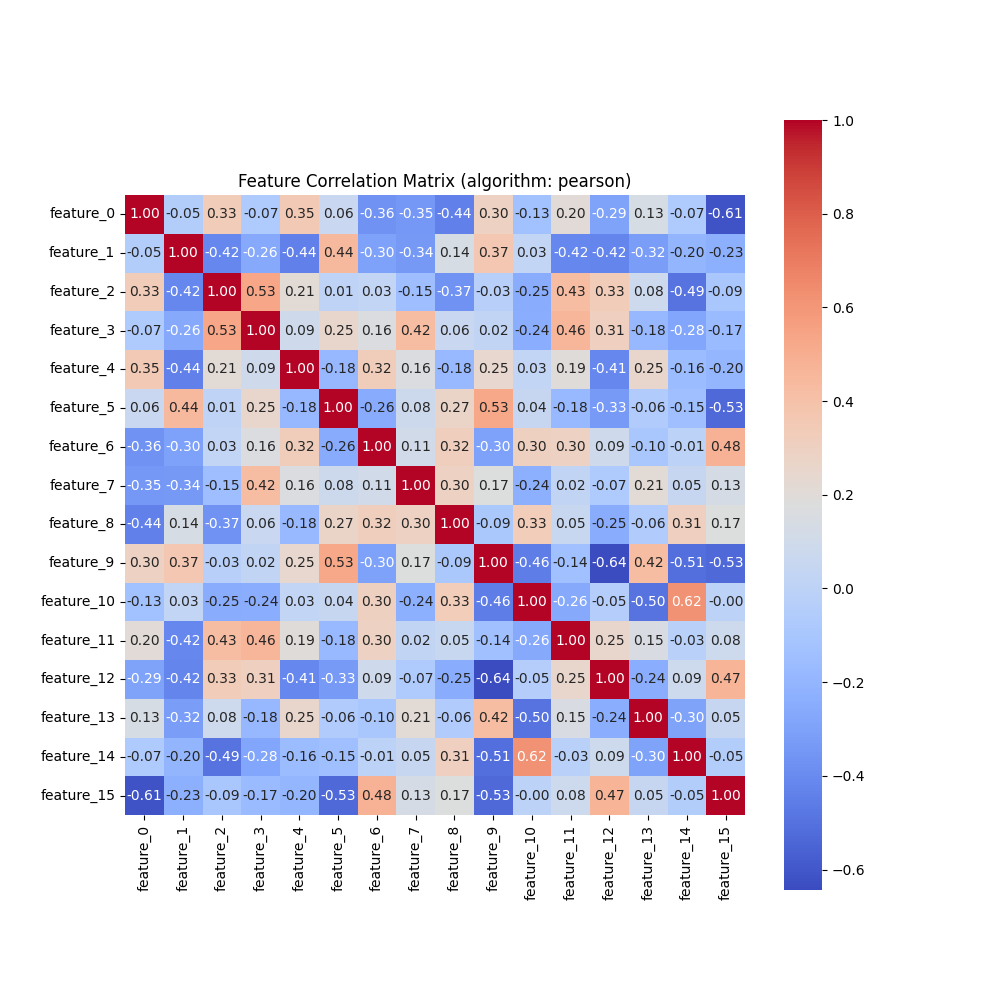
\includegraphics[width=0.8\linewidth]{img/annexes/27_filtered_chunk_extraction_-e_only-max-entropy_-s_activate/Word2vec 4_correlation_matrix.png}} \\
\hline
\end{longtable}


\begin{longtable}{|c|c|}
\caption{Word2vec 5 Feature Engineering Results on 27\_filtered\_chunk\_extraction\_-e\_only-max-entropy\_-s\_activate} \label{tab:27_filtered_chunk_extraction_-e_only-max-entropy_-s_activate_word2vec_5_feature_engineering_results}\\
\hline
Dataset Name & 27\_filtered\_chunk\_extraction\_-e\_only-max-entropy\_-s\_activate \\ \hline
Instance & Word2vec 5 \\ \hline
\multirow{8}{*}{Best Features} & feature\_7 \\ \cline{2-2}
 & feature\_1 \\ \cline{2-2}
 & feature\_13 \\ \cline{2-2}
 & feature\_4 \\ \cline{2-2}
 & feature\_12 \\ \cline{2-2}
 & feature\_5 \\ \cline{2-2}
 & feature\_3 \\ \cline{2-2}
 & feature\_2 \\ \cline{2-2}
\noalign{\vskip 5mm}
\multicolumn{2}{|c|}{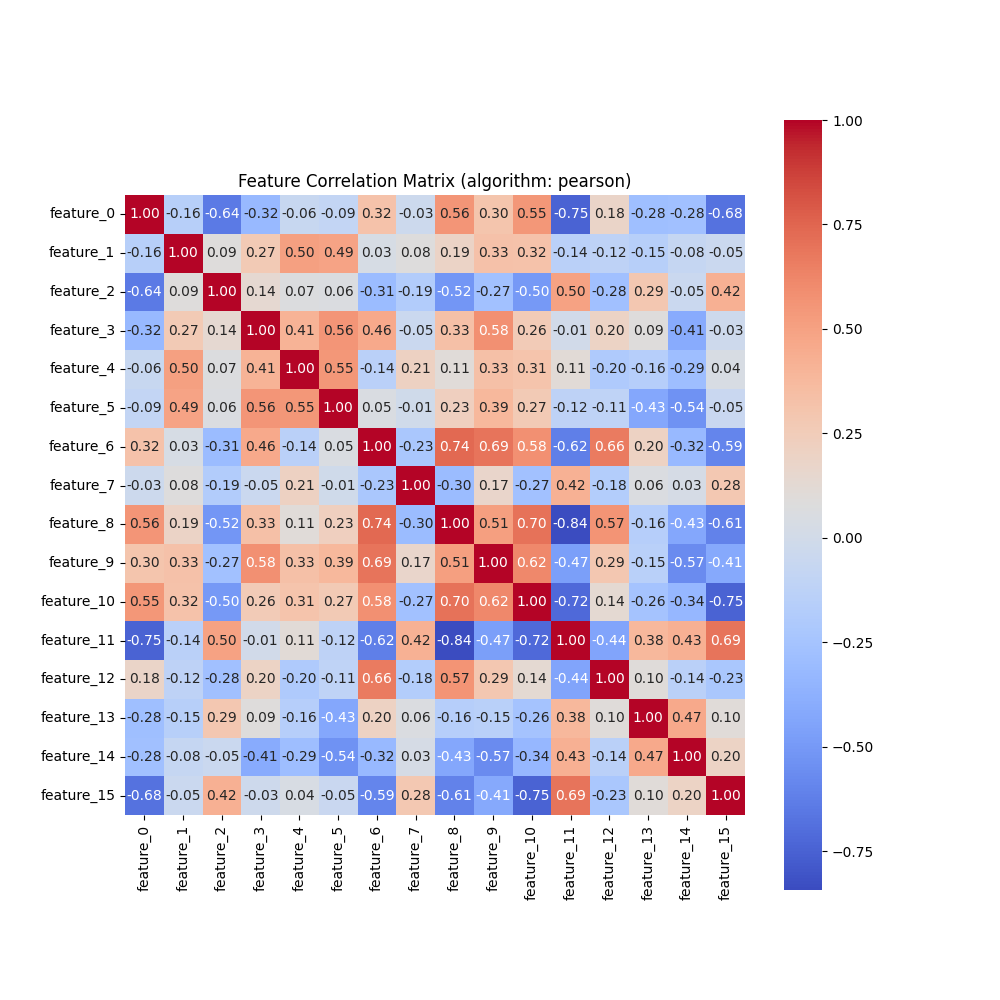
\includegraphics[width=0.8\linewidth]{img/annexes/27_filtered_chunk_extraction_-e_only-max-entropy_-s_activate/Word2vec 5_correlation_matrix.png}} \\
\hline
\end{longtable}


\begin{longtable}{|c|c|}
\caption{Word2vec 8 Feature Engineering Results on 27\_filtered\_chunk\_extraction\_-e\_only-max-entropy\_-s\_activate} \label{tab:27_filtered_chunk_extraction_-e_only-max-entropy_-s_activate_word2vec_8_feature_engineering_results}\\
\hline
Dataset Name & 27\_filtered\_chunk\_extraction\_-e\_only-max-entropy\_-s\_activate \\ \hline
Instance & Word2vec 8 \\ \hline
\multirow{8}{*}{Best Features} & feature\_55 \\ \cline{2-2}
 & feature\_33 \\ \cline{2-2}
 & feature\_25 \\ \cline{2-2}
 & feature\_35 \\ \cline{2-2}
 & feature\_28 \\ \cline{2-2}
 & feature\_32 \\ \cline{2-2}
 & feature\_71 \\ \cline{2-2}
 & feature\_47 \\ \cline{2-2}
\noalign{\vskip 5mm}
\multicolumn{2}{|c|}{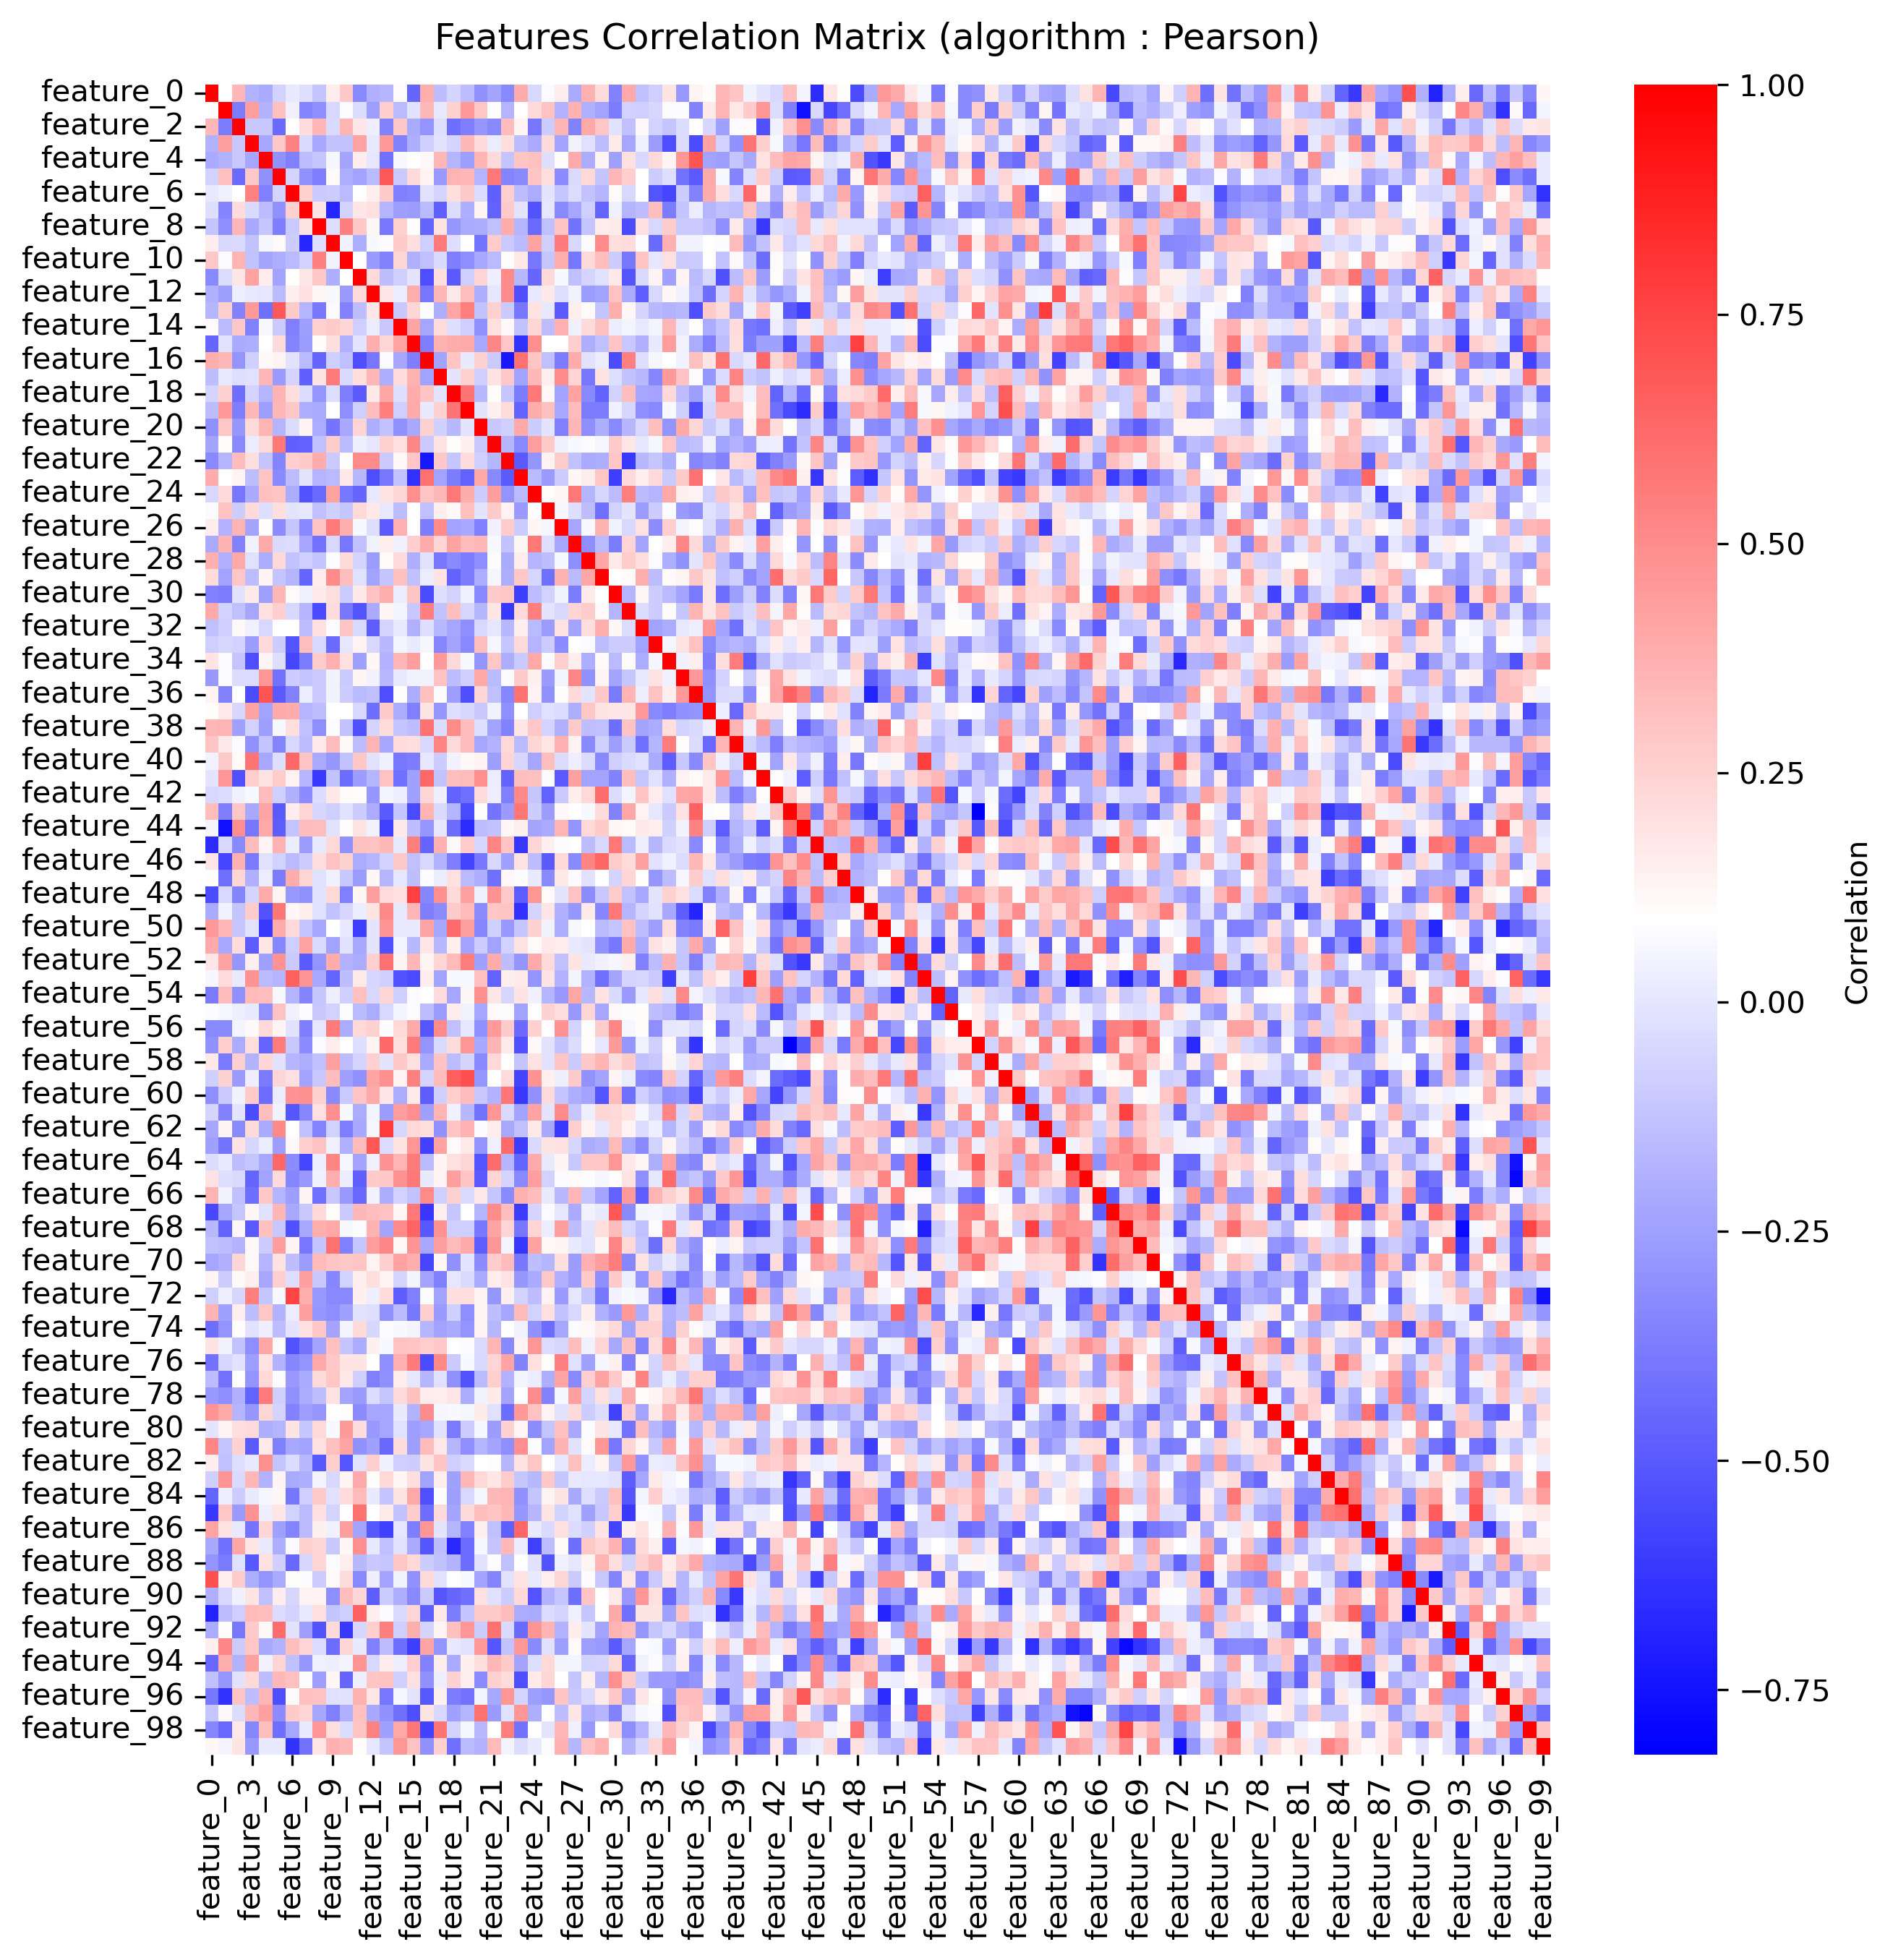
\includegraphics[width=0.8\linewidth]{img/annexes/27_filtered_chunk_extraction_-e_only-max-entropy_-s_activate/Word2vec 8_correlation_matrix.png}} \\
\hline
\end{longtable}


\begin{longtable}{|c|c|}
\caption{Word2vec 9 Feature Engineering Results on 27\_filtered\_chunk\_extraction\_-e\_only-max-entropy\_-s\_activate} \label{tab:27_filtered_chunk_extraction_-e_only-max-entropy_-s_activate_word2vec_9_feature_engineering_results}\\
\hline
Dataset Name & 27\_filtered\_chunk\_extraction\_-e\_only-max-entropy\_-s\_activate \\ \hline
Instance & Word2vec 9 \\ \hline
\multirow{8}{*}{Best Features} & feature\_32 \\ \cline{2-2}
 & feature\_10 \\ \cline{2-2}
 & feature\_14 \\ \cline{2-2}
 & feature\_8 \\ \cline{2-2}
 & feature\_13 \\ \cline{2-2}
 & feature\_28 \\ \cline{2-2}
 & feature\_21 \\ \cline{2-2}
 & feature\_23 \\ \cline{2-2}
\noalign{\vskip 5mm}
\multicolumn{2}{|c|}{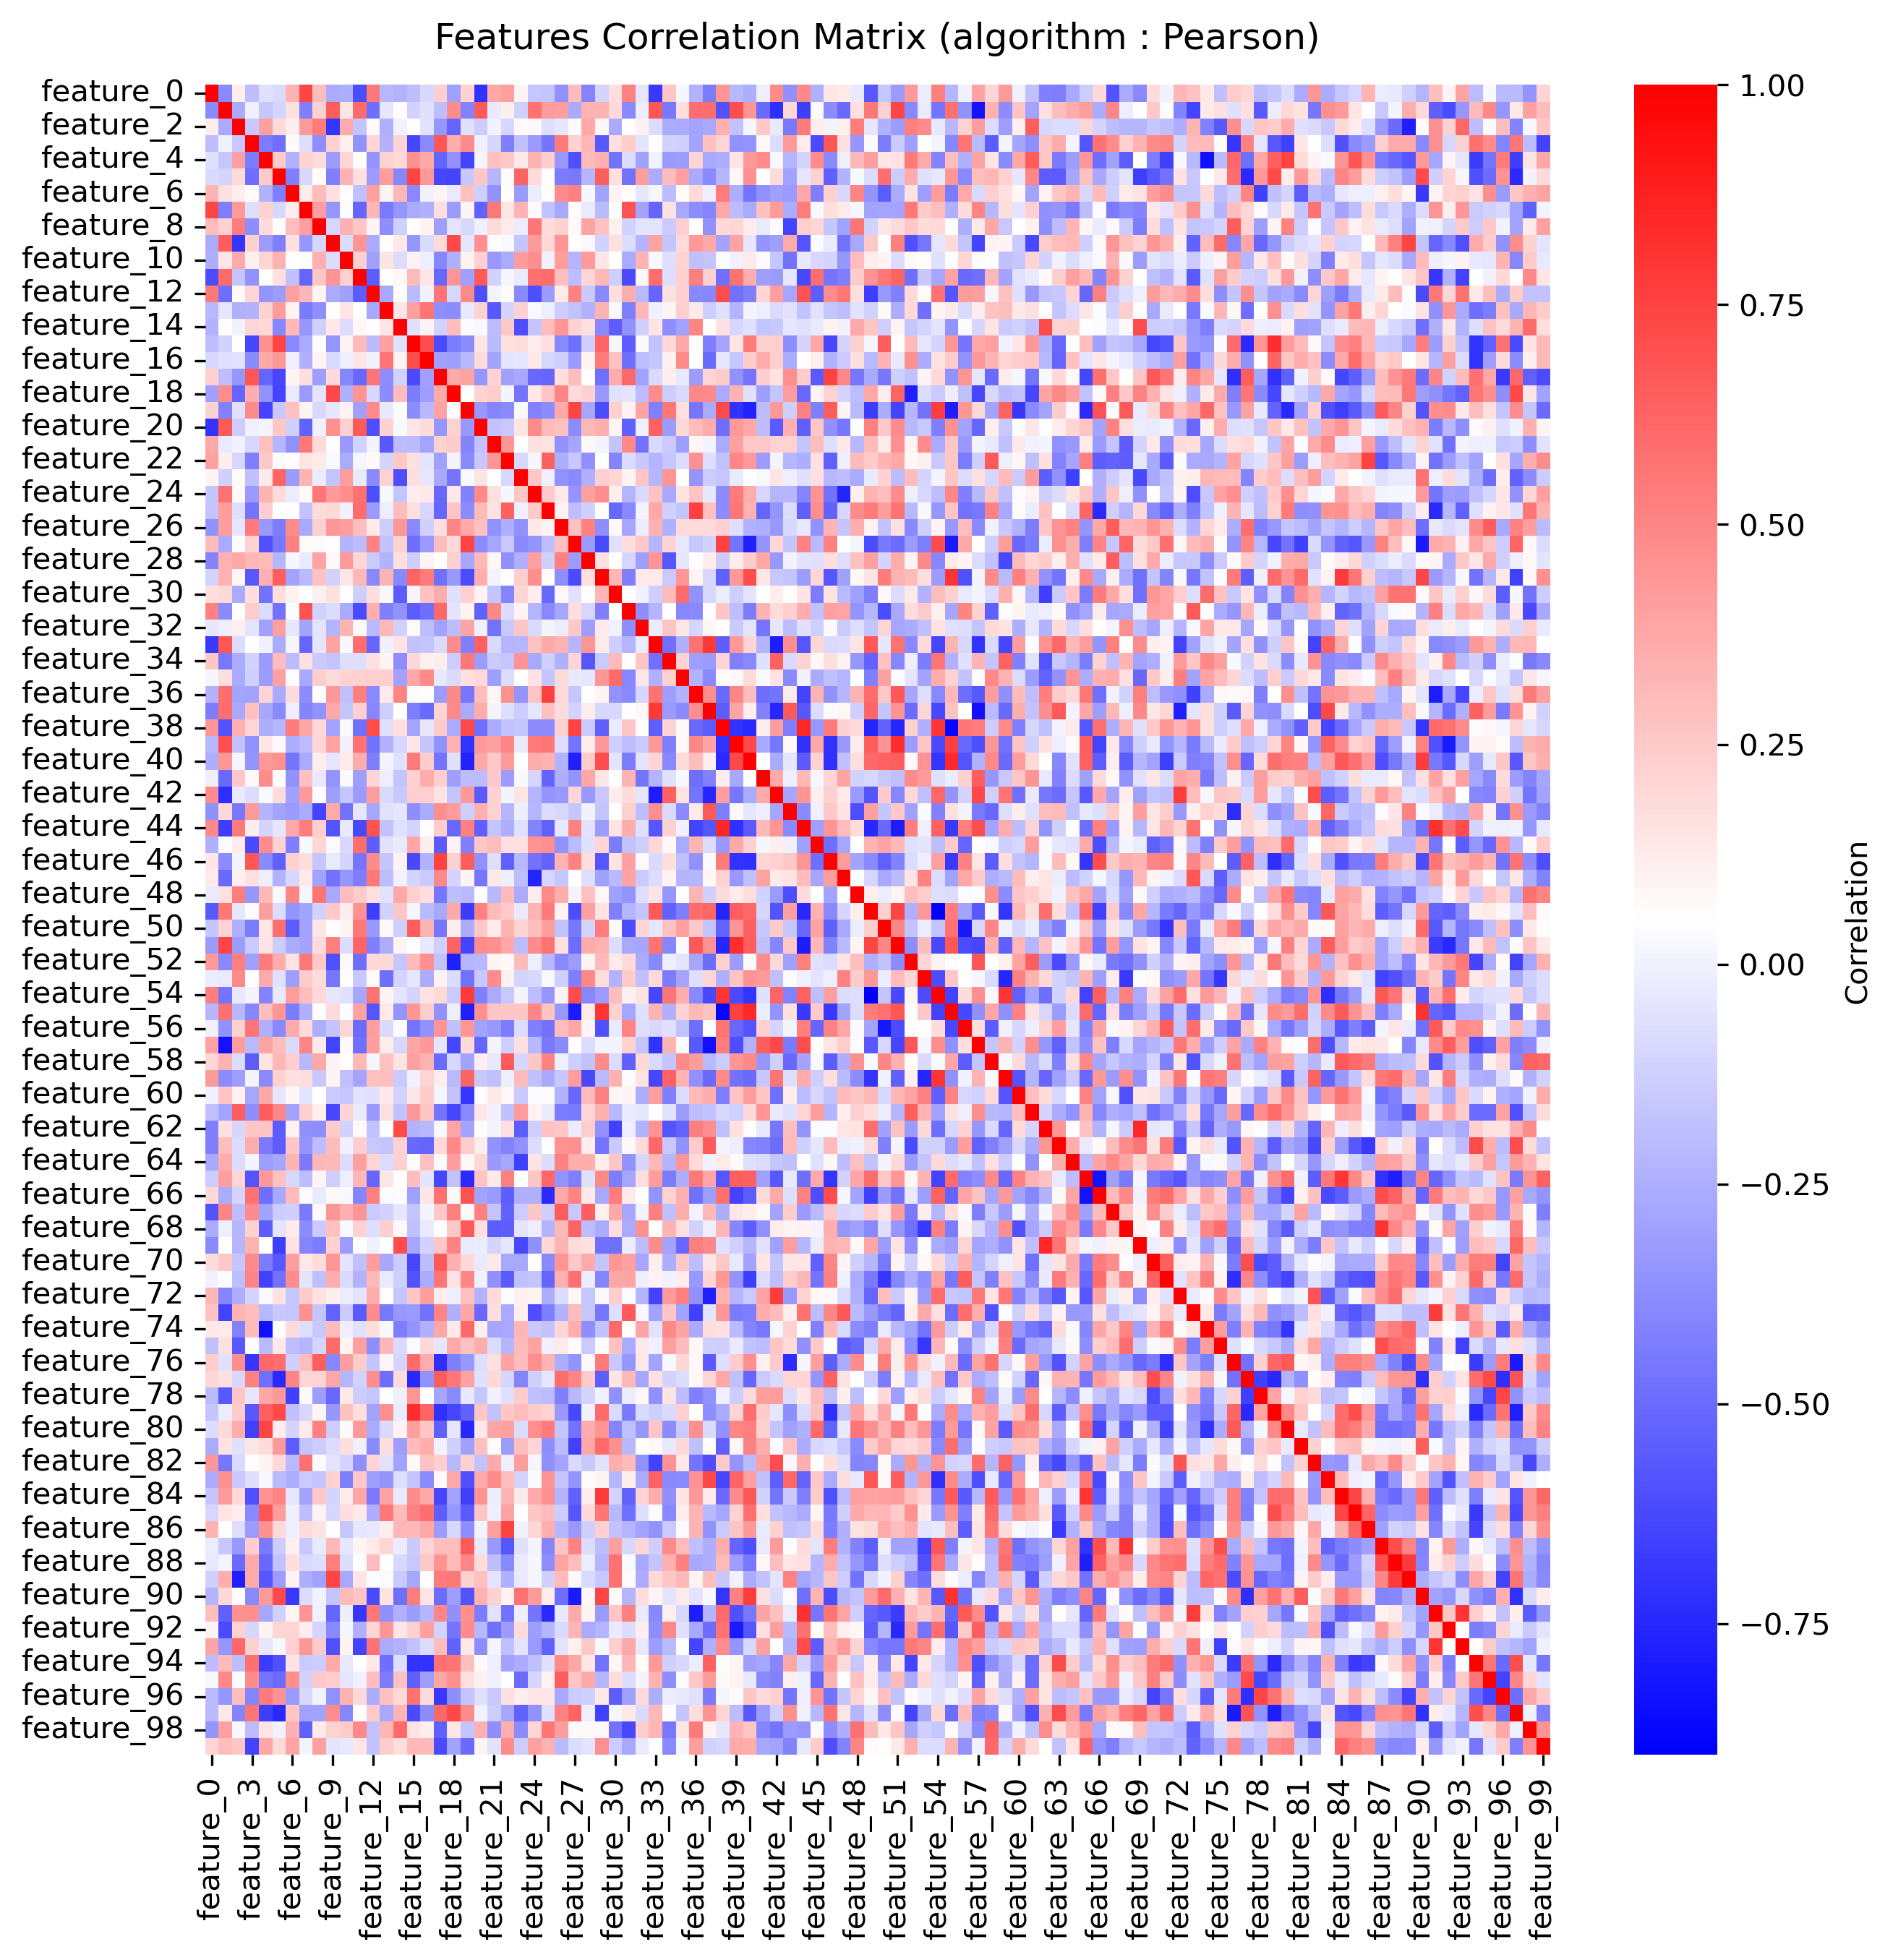
\includegraphics[width=0.8\linewidth]{img/annexes/27_filtered_chunk_extraction_-e_only-max-entropy_-s_activate/Word2vec 9_correlation_matrix.png}} \\
\hline
\end{longtable}


\section{Clustering results}

\label{sec:annexe:clustering_results}

\subsection{26\_filtered\_chunk\_extraction\_-e\_only-max-entropy\_-s\_none}

\begin{longtable}{|c|c|c|c|c|}
\caption{Transformers 0 Clustering Results on 26\_filtered\_chunk\_extraction\_-e\_only-max-entropy\_-s\_none} \label{tab:26_filtered_chunk_extraction_-e_only-max-entropy_-s_none_transformers_0_clustering_results}\\
\hline
\multicolumn{5}{|c|}{\textbf{General Information}} \\
\hline
\multicolumn{2}{|c|}{Min Samples} & \multicolumn{3}{c|}{937} \\
\multicolumn{2}{|c|}{Total Duration} & \multicolumn{3}{c|}{3588.869441 s} \\
\hline
\multicolumn{5}{|c|}{\textbf{Clustering Information}} \\
\hline
EPS & Number of Clusters & Silhouette Score & Noise Points & Duration \\
0.01 & 3 & 0.5749053359031677 & 1369 & 674.16573 s\\
0.02 & 3 & 0.5749053359031677 & 1369 & 664.292675 s\\
0.03 & 3 & 0.574790894985199 & 1371 & 699.778419 s\\
0.04 & 3 & 0.574790894985199 & 1371 & 770.27842 s\\
0.05 & 3 & 0.574790894985199 & 1371 & 776.637103 s\\
\hline
\multicolumn{5}{|c|}{\textbf{Best EPS Information}} \\
\hline
0.01 & 3 & 0.5749053359031677 & 1369 & 674.16573 s\\
\hline
\multicolumn{5}{|c|}{\textbf{Label Association}} \\
\hline
Cluster ID & \multicolumn{2}{c|}{Label} & \multicolumn{2}{c|}{Number of Samples} \\
\hline
\multirow{4}{*}{-1.0} & \multicolumn{2}{c|}{0.0} & \multicolumn{2}{c|}{31} \\
& \multicolumn{2}{c|}{1.0} & \multicolumn{2}{c|}{40} \\
& \multicolumn{2}{c|}{2.0} & \multicolumn{2}{c|}{56} \\
& \multicolumn{2}{c|}{4.0} & \multicolumn{2}{c|}{33} \\
\hline
\multirow{4}{*}{0.0} & \multicolumn{2}{c|}{0.0} & \multicolumn{2}{c|}{35} \\
& \multicolumn{2}{c|}{1.0} & \multicolumn{2}{c|}{40} \\
& \multicolumn{2}{c|}{2.0} & \multicolumn{2}{c|}{26} \\
& \multicolumn{2}{c|}{4.0} & \multicolumn{2}{c|}{32} \\
\hline
\multirow{4}{*}{1.0} & \multicolumn{2}{c|}{0.0} & \multicolumn{2}{c|}{77} \\
& \multicolumn{2}{c|}{1.0} & \multicolumn{2}{c|}{91} \\
& \multicolumn{2}{c|}{2.0} & \multicolumn{2}{c|}{76} \\
& \multicolumn{2}{c|}{4.0} & \multicolumn{2}{c|}{96} \\
\hline
\multirow{4}{*}{2.0} & \multicolumn{2}{c|}{0.0} & \multicolumn{2}{c|}{32} \\
& \multicolumn{2}{c|}{1.0} & \multicolumn{2}{c|}{45} \\
& \multicolumn{2}{c|}{2.0} & \multicolumn{2}{c|}{45} \\
& \multicolumn{2}{c|}{4.0} & \multicolumn{2}{c|}{42} \\
\hline
\end{longtable}


\begin{longtable}{|c|c|c|c|c|}
\caption{Transformers 1 Clustering Results on 26\_filtered\_chunk\_extraction\_-e\_only-max-entropy\_-s\_none} \label{tab:26_filtered_chunk_extraction_-e_only-max-entropy_-s_none_transformers_1_clustering_results}\\
\hline
\multicolumn{5}{|c|}{\textbf{General Information}} \\
\hline
\multicolumn{2}{|c|}{Min Samples} & \multicolumn{3}{c|}{937} \\
\multicolumn{2}{|c|}{Total Duration} & \multicolumn{3}{c|}{3739.406415 s} \\
\hline
\multicolumn{5}{|c|}{\textbf{Clustering Information}} \\
\hline
EPS & Number of Clusters & Silhouette Score & Noise Points & Duration \\
0.01 & 3 & 0.7379494309425354 & 1299 & 760.134469 s\\
0.02 & 3 & 0.7379494309425354 & 1299 & 731.259721 s\\
0.03 & 3 & 0.7379494309425354 & 1299 & 738.923279 s\\
0.04 & 3 & 0.7379494309425354 & 1299 & 761.430407 s\\
0.05 & 3 & 0.3740614056587219 & 2696 & 743.313265 s\\
\hline
\multicolumn{5}{|c|}{\textbf{Best EPS Information}} \\
\hline
0.01 & 3 & 0.7379494309425354 & 1299 & 760.134469 s\\
\hline
\multicolumn{5}{|c|}{\textbf{Label Association}} \\
\hline
Cluster ID & \multicolumn{2}{c|}{Label} & \multicolumn{2}{c|}{Number of Samples} \\
\hline
\multirow{4}{*}{-1.0} & \multicolumn{2}{c|}{0.0} & \multicolumn{2}{c|}{29} \\
& \multicolumn{2}{c|}{1.0} & \multicolumn{2}{c|}{37} \\
& \multicolumn{2}{c|}{2.0} & \multicolumn{2}{c|}{56} \\
& \multicolumn{2}{c|}{4.0} & \multicolumn{2}{c|}{32} \\
\hline
\multirow{4}{*}{0.0} & \multicolumn{2}{c|}{0.0} & \multicolumn{2}{c|}{37} \\
& \multicolumn{2}{c|}{1.0} & \multicolumn{2}{c|}{43} \\
& \multicolumn{2}{c|}{2.0} & \multicolumn{2}{c|}{26} \\
& \multicolumn{2}{c|}{4.0} & \multicolumn{2}{c|}{33} \\
\hline
\multirow{4}{*}{1.0} & \multicolumn{2}{c|}{0.0} & \multicolumn{2}{c|}{77} \\
& \multicolumn{2}{c|}{1.0} & \multicolumn{2}{c|}{91} \\
& \multicolumn{2}{c|}{2.0} & \multicolumn{2}{c|}{76} \\
& \multicolumn{2}{c|}{4.0} & \multicolumn{2}{c|}{96} \\
\hline
\multirow{4}{*}{2.0} & \multicolumn{2}{c|}{0.0} & \multicolumn{2}{c|}{32} \\
& \multicolumn{2}{c|}{1.0} & \multicolumn{2}{c|}{45} \\
& \multicolumn{2}{c|}{2.0} & \multicolumn{2}{c|}{45} \\
& \multicolumn{2}{c|}{4.0} & \multicolumn{2}{c|}{42} \\
\hline
\end{longtable}


\begin{longtable}{|c|c|c|c|c|}
\caption{Word2vec 0 Clustering Results on 26\_filtered\_chunk\_extraction\_-e\_only-max-entropy\_-s\_none} \label{tab:26_filtered_chunk_extraction_-e_only-max-entropy_-s_none_word2vec_0_clustering_results}\\
\hline
\multicolumn{5}{|c|}{\textbf{General Information}} \\
\hline
\multicolumn{2}{|c|}{Min Samples} & \multicolumn{3}{c|}{937} \\
\multicolumn{2}{|c|}{Total Duration} & \multicolumn{3}{c|}{4670.078544 s} \\
\hline
\multicolumn{5}{|c|}{\textbf{Clustering Information}} \\
\hline
EPS & Number of Clusters & Silhouette Score & Noise Points & Duration \\
0.01 & 1 & None & None & 936.207143 s\\
0.02 & 1 & None & None & 869.910205 s\\
0.03 & 1 & None & None & 948.106213 s\\
0.04 & 1 & None & None & 961.156023 s\\
0.05 & 1 & None & None & 954.667794 s\\
\hline
\multicolumn{5}{|c|}{\textbf{Label Association}} \\
\hline
Cluster ID & \multicolumn{2}{c|}{Label} & \multicolumn{2}{c|}{Number of Samples} \\
\hline
\end{longtable}


\begin{longtable}{|c|c|c|c|c|}
\caption{Word2vec 1 Clustering Results on 26\_filtered\_chunk\_extraction\_-e\_only-max-entropy\_-s\_none} \label{tab:26_filtered_chunk_extraction_-e_only-max-entropy_-s_none_word2vec_1_clustering_results}\\
\hline
\multicolumn{5}{|c|}{\textbf{General Information}} \\
\hline
\multicolumn{2}{|c|}{Min Samples} & \multicolumn{3}{c|}{937} \\
\multicolumn{2}{|c|}{Total Duration} & \multicolumn{3}{c|}{4290.037825 s} \\
\hline
\multicolumn{5}{|c|}{\textbf{Clustering Information}} \\
\hline
EPS & Number of Clusters & Silhouette Score & Noise Points & Duration \\
0.01 & 1 & None & None & 934.991492 s\\
0.02 & 1 & None & None & 866.160618 s\\
0.03 & 1 & None & None & 842.744876 s\\
0.04 & 1 & None & None & 826.449586 s\\
0.05 & 1 & None & None & 819.657228 s\\
\hline
\multicolumn{5}{|c|}{\textbf{Label Association}} \\
\hline
Cluster ID & \multicolumn{2}{c|}{Label} & \multicolumn{2}{c|}{Number of Samples} \\
\hline
\end{longtable}


\begin{longtable}{|c|c|c|c|c|}
\caption{Word2vec 4 Clustering Results on 26\_filtered\_chunk\_extraction\_-e\_only-max-entropy\_-s\_none} \label{tab:26_filtered_chunk_extraction_-e_only-max-entropy_-s_none_word2vec_4_clustering_results}\\
\hline
\multicolumn{5}{|c|}{\textbf{General Information}} \\
\hline
\multicolumn{2}{|c|}{Min Samples} & \multicolumn{3}{c|}{937} \\
\multicolumn{2}{|c|}{Total Duration} & \multicolumn{3}{c|}{4935.790898 s} \\
\hline
\multicolumn{5}{|c|}{\textbf{Clustering Information}} \\
\hline
EPS & Number of Clusters & Silhouette Score & Noise Points & Duration \\
0.01 & 1 & None & None & 918.607782 s\\
0.02 & 1 & None & None & 1025.651433 s\\
0.03 & 1 & None & None & 964.72504 s\\
0.04 & 1 & None & None & 1037.539299 s\\
0.05 & 1 & None & None & 989.228145 s\\
\hline
\multicolumn{5}{|c|}{\textbf{Label Association}} \\
\hline
Cluster ID & \multicolumn{2}{c|}{Label} & \multicolumn{2}{c|}{Number of Samples} \\
\hline
\end{longtable}


\begin{longtable}{|c|c|c|c|c|}
\caption{Word2vec 5 Clustering Results on 26\_filtered\_chunk\_extraction\_-e\_only-max-entropy\_-s\_none} \label{tab:26_filtered_chunk_extraction_-e_only-max-entropy_-s_none_word2vec_5_clustering_results}\\
\hline
\multicolumn{5}{|c|}{\textbf{General Information}} \\
\hline
\multicolumn{2}{|c|}{Min Samples} & \multicolumn{3}{c|}{937} \\
\multicolumn{2}{|c|}{Total Duration} & \multicolumn{3}{c|}{4306.497069 s} \\
\hline
\multicolumn{5}{|c|}{\textbf{Clustering Information}} \\
\hline
EPS & Number of Clusters & Silhouette Score & Noise Points & Duration \\
0.01 & 1 & None & None & 872.005797 s\\
0.02 & 1 & None & None & 813.355077 s\\
0.03 & 1 & None & None & 863.573455 s\\
0.04 & 1 & None & None & 857.413105 s\\
0.05 & 1 & None & None & 900.115125 s\\
\hline
\multicolumn{5}{|c|}{\textbf{Label Association}} \\
\hline
Cluster ID & \multicolumn{2}{c|}{Label} & \multicolumn{2}{c|}{Number of Samples} \\
\hline
\end{longtable}


\begin{longtable}{|c|c|c|c|c|}
\caption{Word2vec 8 Clustering Results on 26\_filtered\_chunk\_extraction\_-e\_only-max-entropy\_-s\_none} \label{tab:26_filtered_chunk_extraction_-e_only-max-entropy_-s_none_word2vec_8_clustering_results}\\
\hline
\multicolumn{5}{|c|}{\textbf{General Information}} \\
\hline
\multicolumn{2}{|c|}{Min Samples} & \multicolumn{3}{c|}{937} \\
\multicolumn{2}{|c|}{Total Duration} & \multicolumn{3}{c|}{4849.607168 s} \\
\hline
\multicolumn{5}{|c|}{\textbf{Clustering Information}} \\
\hline
EPS & Number of Clusters & Silhouette Score & Noise Points & Duration \\
0.01 & 1 & None & None & 958.117555 s\\
0.02 & 1 & None & None & 936.954803 s\\
0.03 & 1 & None & None & 979.485905 s\\
0.04 & 1 & None & None & 956.620507 s\\
0.05 & 1 & None & None & 1018.395839 s\\
\hline
\multicolumn{5}{|c|}{\textbf{Label Association}} \\
\hline
Cluster ID & \multicolumn{2}{c|}{Label} & \multicolumn{2}{c|}{Number of Samples} \\
\hline
\end{longtable}


\begin{longtable}{|c|c|c|c|c|}
\caption{Word2vec 9 Clustering Results on 26\_filtered\_chunk\_extraction\_-e\_only-max-entropy\_-s\_none} \label{tab:26_filtered_chunk_extraction_-e_only-max-entropy_-s_none_word2vec_9_clustering_results}\\
\hline
\multicolumn{5}{|c|}{\textbf{General Information}} \\
\hline
\multicolumn{2}{|c|}{Min Samples} & \multicolumn{3}{c|}{937} \\
\multicolumn{2}{|c|}{Total Duration} & \multicolumn{3}{c|}{4526.462559 s} \\
\hline
\multicolumn{5}{|c|}{\textbf{Clustering Information}} \\
\hline
EPS & Number of Clusters & Silhouette Score & Noise Points & Duration \\
0.01 & 1 & None & None & 937.229162 s\\
0.02 & 1 & None & None & 866.822815 s\\
0.03 & 1 & None & None & 915.390656 s\\
0.04 & 1 & None & None & 895.444037 s\\
0.05 & 1 & None & None & 911.542842 s\\
\hline
\multicolumn{5}{|c|}{\textbf{Label Association}} \\
\hline
Cluster ID & \multicolumn{2}{c|}{Label} & \multicolumn{2}{c|}{Number of Samples} \\
\hline
\end{longtable}


\subsection{27\_filtered\_chunk\_extraction\_-e\_only-max-entropy\_-s\_activate}

\begin{longtable}{|c|c|c|c|c|}
\caption{Transformers 0 Clustering Results on 27\_filtered\_chunk\_extraction\_-e\_only-max-entropy\_-s\_activate} \label{tab:27_filtered_chunk_extraction_-e_only-max-entropy_-s_activate_transformers_0_clustering_results}\\
\hline
\multicolumn{5}{|c|}{\textbf{General Information}} \\
\hline
\multicolumn{2}{|c|}{Min Samples} & \multicolumn{3}{c|}{937} \\
\multicolumn{2}{|c|}{Total Duration} & \multicolumn{3}{c|}{3796.324605 s} \\
\hline
\multicolumn{5}{|c|}{\textbf{Clustering Information}} \\
\hline
EPS & Number of Clusters & Silhouette Score & Noise Points & Duration \\
0.01 & 3 & 0.2465989887714386 & 2274 & 709.617939 s\\
0.02 & 3 & 0.24514129757881165 & 2281 & 753.217155 s\\
0.03 & 2 & 0.1906411200761795 & 3242 & 820.552446 s\\
0.04 & 2 & 0.1906411200761795 & 3242 & 756.897654 s\\
0.05 & 2 & 0.1906411200761795 & 3242 & 751.836631 s\\
\hline
\multicolumn{5}{|c|}{\textbf{Best EPS Information}} \\
\hline
0.01 & 3 & 0.2465989887714386 & 2274 & 709.617939 s\\
\hline
\multicolumn{5}{|c|}{\textbf{Label Association}} \\
\hline
Cluster ID & \multicolumn{2}{c|}{Label} & \multicolumn{2}{c|}{Number of Samples} \\
\hline
\multirow{4}{*}{-1.0} & \multicolumn{2}{c|}{0.0} & \multicolumn{2}{c|}{91} \\
& \multicolumn{2}{c|}{1.0} & \multicolumn{2}{c|}{95} \\
& \multicolumn{2}{c|}{2.0} & \multicolumn{2}{c|}{99} \\
& \multicolumn{2}{c|}{4.0} & \multicolumn{2}{c|}{97} \\
\hline
\multirow{4}{*}{0.0} & \multicolumn{2}{c|}{0.0} & \multicolumn{2}{c|}{128} \\
& \multicolumn{2}{c|}{1.0} & \multicolumn{2}{c|}{129} \\
& \multicolumn{2}{c|}{2.0} & \multicolumn{2}{c|}{94} \\
& \multicolumn{2}{c|}{4.0} & \multicolumn{2}{c|}{110} \\
\hline
\multirow{4}{*}{1.0} & \multicolumn{2}{c|}{0.0} & \multicolumn{2}{c|}{50} \\
& \multicolumn{2}{c|}{1.0} & \multicolumn{2}{c|}{40} \\
& \multicolumn{2}{c|}{2.0} & \multicolumn{2}{c|}{44} \\
& \multicolumn{2}{c|}{4.0} & \multicolumn{2}{c|}{33} \\
\hline
\multirow{4}{*}{2.0} & \multicolumn{2}{c|}{0.0} & \multicolumn{2}{c|}{52} \\
& \multicolumn{2}{c|}{1.0} & \multicolumn{2}{c|}{51} \\
& \multicolumn{2}{c|}{2.0} & \multicolumn{2}{c|}{53} \\
& \multicolumn{2}{c|}{4.0} & \multicolumn{2}{c|}{50} \\
\hline
\end{longtable}


\begin{longtable}{|c|c|c|c|c|}
\caption{Transformers 1 Clustering Results on 27\_filtered\_chunk\_extraction\_-e\_only-max-entropy\_-s\_activate} \label{tab:27_filtered_chunk_extraction_-e_only-max-entropy_-s_activate_transformers_1_clustering_results}\\
\hline
\multicolumn{5}{|c|}{\textbf{General Information}} \\
\hline
\multicolumn{2}{|c|}{Min Samples} & \multicolumn{3}{c|}{937} \\
\multicolumn{2}{|c|}{Total Duration} & \multicolumn{3}{c|}{3943.383724 s} \\
\hline
\multicolumn{5}{|c|}{\textbf{Clustering Information}} \\
\hline
EPS & Number of Clusters & Silhouette Score & Noise Points & Duration \\
0.01 & 4 & 0.5144023299217224 & 981 & 810.887225 s\\
0.02 & 3 & 0.8070926070213318 & 533 & 798.792131 s\\
0.03 & 3 & 0.8070926070213318 & 533 & 772.422919 s\\
0.04 & 3 & 0.8070926070213318 & 533 & 775.663572 s\\
0.05 & 3 & 0.8070926070213318 & 533 & 781.48437 s\\
\hline
\multicolumn{5}{|c|}{\textbf{Best EPS Information}} \\
\hline
0.02 & 3 & 0.8070926070213318 & 533 & 798.792131 s\\
\hline
\multicolumn{5}{|c|}{\textbf{Label Association}} \\
\hline
Cluster ID & \multicolumn{2}{c|}{Label} & \multicolumn{2}{c|}{Number of Samples} \\
\hline
\multirow{4}{*}{-1.0} & \multicolumn{2}{c|}{0.0} & \multicolumn{2}{c|}{19} \\
& \multicolumn{2}{c|}{1.0} & \multicolumn{2}{c|}{20} \\
& \multicolumn{2}{c|}{2.0} & \multicolumn{2}{c|}{20} \\
& \multicolumn{2}{c|}{4.0} & \multicolumn{2}{c|}{20} \\
\hline
\multirow{4}{*}{0.0} & \multicolumn{2}{c|}{0.0} & \multicolumn{2}{c|}{182} \\
& \multicolumn{2}{c|}{1.0} & \multicolumn{2}{c|}{155} \\
& \multicolumn{2}{c|}{2.0} & \multicolumn{2}{c|}{138} \\
& \multicolumn{2}{c|}{4.0} & \multicolumn{2}{c|}{145} \\
\hline
\multirow{4}{*}{1.0} & \multicolumn{2}{c|}{0.0} & \multicolumn{2}{c|}{74} \\
& \multicolumn{2}{c|}{1.0} & \multicolumn{2}{c|}{96} \\
& \multicolumn{2}{c|}{2.0} & \multicolumn{2}{c|}{81} \\
& \multicolumn{2}{c|}{4.0} & \multicolumn{2}{c|}{85} \\
\hline
\multirow{4}{*}{2.0} & \multicolumn{2}{c|}{0.0} & \multicolumn{2}{c|}{46} \\
& \multicolumn{2}{c|}{1.0} & \multicolumn{2}{c|}{44} \\
& \multicolumn{2}{c|}{2.0} & \multicolumn{2}{c|}{51} \\
& \multicolumn{2}{c|}{4.0} & \multicolumn{2}{c|}{40} \\
\hline
\end{longtable}


\begin{longtable}{|c|c|c|c|c|}
\caption{Transformers 2 Clustering Results on 27\_filtered\_chunk\_extraction\_-e\_only-max-entropy\_-s\_activate} \label{tab:27_filtered_chunk_extraction_-e_only-max-entropy_-s_activate_transformers_2_clustering_results}\\
\hline
\multicolumn{5}{|c|}{\textbf{General Information}} \\
\hline
\multicolumn{2}{|c|}{Min Samples} & \multicolumn{3}{c|}{937} \\
\multicolumn{2}{|c|}{Total Duration} & \multicolumn{3}{c|}{3895.618311 s} \\
\hline
\multicolumn{5}{|c|}{\textbf{Clustering Information}} \\
\hline
EPS & Number of Clusters & Silhouette Score & Noise Points & Duration \\
0.01 & 2 & 0.907838761806488 & 0 & 790.283896 s\\
0.02 & 2 & 0.907838761806488 & 0 & 802.295121 s\\
0.03 & 2 & 0.907838761806488 & 0 & 787.142639 s\\
0.04 & 2 & 0.907838761806488 & 0 & 725.182204 s\\
0.05 & 2 & 0.907838761806488 & 0 & 785.995246 s\\
\hline
\multicolumn{5}{|c|}{\textbf{Best EPS Information}} \\
\hline
0.01 & 2 & 0.907838761806488 & 0 & 790.283896 s\\
\hline
\multicolumn{5}{|c|}{\textbf{Label Association}} \\
\hline
Cluster ID & \multicolumn{2}{c|}{Label} & \multicolumn{2}{c|}{Number of Samples} \\
\hline
\multirow{4}{*}{0.0} & \multicolumn{2}{c|}{0.0} & \multicolumn{2}{c|}{264} \\
& \multicolumn{2}{c|}{1.0} & \multicolumn{2}{c|}{256} \\
& \multicolumn{2}{c|}{2.0} & \multicolumn{2}{c|}{228} \\
& \multicolumn{2}{c|}{4.0} & \multicolumn{2}{c|}{236} \\
\hline
\multirow{4}{*}{1.0} & \multicolumn{2}{c|}{0.0} & \multicolumn{2}{c|}{57} \\
& \multicolumn{2}{c|}{1.0} & \multicolumn{2}{c|}{59} \\
& \multicolumn{2}{c|}{2.0} & \multicolumn{2}{c|}{62} \\
& \multicolumn{2}{c|}{4.0} & \multicolumn{2}{c|}{54} \\
\hline
\end{longtable}


\begin{longtable}{|c|c|c|c|c|}
\caption{Transformers 3 Clustering Results on 27\_filtered\_chunk\_extraction\_-e\_only-max-entropy\_-s\_activate} \label{tab:27_filtered_chunk_extraction_-e_only-max-entropy_-s_activate_transformers_3_clustering_results}\\
\hline
\multicolumn{5}{|c|}{\textbf{General Information}} \\
\hline
\multicolumn{2}{|c|}{Min Samples} & \multicolumn{3}{c|}{937} \\
\multicolumn{2}{|c|}{Total Duration} & \multicolumn{3}{c|}{3939.333846 s} \\
\hline
\multicolumn{5}{|c|}{\textbf{Clustering Information}} \\
\hline
EPS & Number of Clusters & Silhouette Score & Noise Points & Duration \\
0.01 & 3 & 0.36908280849456787 & 2637 & 806.707338 s\\
0.02 & 3 & 0.36908280849456787 & 2637 & 782.581847 s\\
0.03 & 3 & 0.36908280849456787 & 2637 & 775.659231 s\\
0.04 & 3 & 0.36908280849456787 & 2637 & 783.727976 s\\
0.05 & 3 & 0.36908280849456787 & 2637 & 786.255646 s\\
\hline
\multicolumn{5}{|c|}{\textbf{Best EPS Information}} \\
\hline
0.01 & 3 & 0.36908280849456787 & 2637 & 806.707338 s\\
\hline
\multicolumn{5}{|c|}{\textbf{Label Association}} \\
\hline
Cluster ID & \multicolumn{2}{c|}{Label} & \multicolumn{2}{c|}{Number of Samples} \\
\hline
\multirow{4}{*}{-1.0} & \multicolumn{2}{c|}{0.0} & \multicolumn{2}{c|}{134} \\
& \multicolumn{2}{c|}{1.0} & \multicolumn{2}{c|}{97} \\
& \multicolumn{2}{c|}{2.0} & \multicolumn{2}{c|}{114} \\
& \multicolumn{2}{c|}{4.0} & \multicolumn{2}{c|}{111} \\
\hline
\multirow{4}{*}{0.0} & \multicolumn{2}{c|}{0.0} & \multicolumn{2}{c|}{81} \\
& \multicolumn{2}{c|}{1.0} & \multicolumn{2}{c|}{86} \\
& \multicolumn{2}{c|}{2.0} & \multicolumn{2}{c|}{53} \\
& \multicolumn{2}{c|}{4.0} & \multicolumn{2}{c|}{72} \\
\hline
\multirow{4}{*}{1.0} & \multicolumn{2}{c|}{0.0} & \multicolumn{2}{c|}{49} \\
& \multicolumn{2}{c|}{1.0} & \multicolumn{2}{c|}{73} \\
& \multicolumn{2}{c|}{2.0} & \multicolumn{2}{c|}{61} \\
& \multicolumn{2}{c|}{4.0} & \multicolumn{2}{c|}{53} \\
\hline
\multirow{4}{*}{2.0} & \multicolumn{2}{c|}{0.0} & \multicolumn{2}{c|}{57} \\
& \multicolumn{2}{c|}{1.0} & \multicolumn{2}{c|}{59} \\
& \multicolumn{2}{c|}{2.0} & \multicolumn{2}{c|}{62} \\
& \multicolumn{2}{c|}{4.0} & \multicolumn{2}{c|}{54} \\
\hline
\end{longtable}


\begin{longtable}{|c|c|c|c|c|}
\caption{Transformers 4 Clustering Results on 27\_filtered\_chunk\_extraction\_-e\_only-max-entropy\_-s\_activate} \label{tab:27_filtered_chunk_extraction_-e_only-max-entropy_-s_activate_transformers_4_clustering_results}\\
\hline
\multicolumn{5}{|c|}{\textbf{General Information}} \\
\hline
\multicolumn{2}{|c|}{Min Samples} & \multicolumn{3}{c|}{937} \\
\multicolumn{2}{|c|}{Total Duration} & \multicolumn{3}{c|}{3803.240679 s} \\
\hline
\multicolumn{5}{|c|}{\textbf{Clustering Information}} \\
\hline
EPS & Number of Clusters & Silhouette Score & Noise Points & Duration \\
0.01 & 3 & 0.6185895800590515 & 1103 & 794.276663 s\\
0.02 & 3 & 0.6185895800590515 & 1103 & 746.079328 s\\
0.03 & 3 & 0.6186758875846863 & 1105 & 737.198024 s\\
0.04 & 2 & 0.47322237491607666 & 2390 & 732.879635 s\\
0.05 & 2 & 0.47322237491607666 & 2390 & 788.087243 s\\
\hline
\multicolumn{5}{|c|}{\textbf{Best EPS Information}} \\
\hline
0.03 & 3 & 0.6186758875846863 & 1105 & 737.198024 s\\
\hline
\multicolumn{5}{|c|}{\textbf{Label Association}} \\
\hline
Cluster ID & \multicolumn{2}{c|}{Label} & \multicolumn{2}{c|}{Number of Samples} \\
\hline
\multirow{4}{*}{-1.0} & \multicolumn{2}{c|}{0.0} & \multicolumn{2}{c|}{44} \\
& \multicolumn{2}{c|}{1.0} & \multicolumn{2}{c|}{43} \\
& \multicolumn{2}{c|}{2.0} & \multicolumn{2}{c|}{43} \\
& \multicolumn{2}{c|}{4.0} & \multicolumn{2}{c|}{53} \\
\hline
\multirow{4}{*}{0.0} & \multicolumn{2}{c|}{0.0} & \multicolumn{2}{c|}{184} \\
& \multicolumn{2}{c|}{1.0} & \multicolumn{2}{c|}{159} \\
& \multicolumn{2}{c|}{2.0} & \multicolumn{2}{c|}{140} \\
& \multicolumn{2}{c|}{4.0} & \multicolumn{2}{c|}{146} \\
\hline
\multirow{4}{*}{1.0} & \multicolumn{2}{c|}{0.0} & \multicolumn{2}{c|}{47} \\
& \multicolumn{2}{c|}{1.0} & \multicolumn{2}{c|}{69} \\
& \multicolumn{2}{c|}{2.0} & \multicolumn{2}{c|}{59} \\
& \multicolumn{2}{c|}{4.0} & \multicolumn{2}{c|}{52} \\
\hline
\multirow{4}{*}{2.0} & \multicolumn{2}{c|}{0.0} & \multicolumn{2}{c|}{46} \\
& \multicolumn{2}{c|}{1.0} & \multicolumn{2}{c|}{44} \\
& \multicolumn{2}{c|}{2.0} & \multicolumn{2}{c|}{48} \\
& \multicolumn{2}{c|}{4.0} & \multicolumn{2}{c|}{39} \\
\hline
\end{longtable}


\begin{longtable}{|c|c|c|c|c|}
\caption{Transformers 5 Clustering Results on 27\_filtered\_chunk\_extraction\_-e\_only-max-entropy\_-s\_activate} \label{tab:27_filtered_chunk_extraction_-e_only-max-entropy_-s_activate_transformers_5_clustering_results}\\
\hline
\multicolumn{5}{|c|}{\textbf{General Information}} \\
\hline
\multicolumn{2}{|c|}{Min Samples} & \multicolumn{3}{c|}{937} \\
\multicolumn{2}{|c|}{Total Duration} & \multicolumn{3}{c|}{3935.993827 s} \\
\hline
\multicolumn{5}{|c|}{\textbf{Clustering Information}} \\
\hline
EPS & Number of Clusters & Silhouette Score & Noise Points & Duration \\
0.01 & 1 & None & None & 764.413697 s\\
0.02 & 1 & None & None & 783.772212 s\\
0.03 & 1 & None & None & 811.087261 s\\
0.04 & 1 & None & None & 772.993991 s\\
0.05 & 1 & None & None & 803.689671 s\\
\hline
\multicolumn{5}{|c|}{\textbf{Label Association}} \\
\hline
Cluster ID & \multicolumn{2}{c|}{Label} & \multicolumn{2}{c|}{Number of Samples} \\
\hline
\end{longtable}


\begin{longtable}{|c|c|c|c|c|}
\caption{Transformers 6 Clustering Results on 27\_filtered\_chunk\_extraction\_-e\_only-max-entropy\_-s\_activate} \label{tab:27_filtered_chunk_extraction_-e_only-max-entropy_-s_activate_transformers_6_clustering_results}\\
\hline
\multicolumn{5}{|c|}{\textbf{General Information}} \\
\hline
\multicolumn{2}{|c|}{Min Samples} & \multicolumn{3}{c|}{937} \\
\multicolumn{2}{|c|}{Total Duration} & \multicolumn{3}{c|}{3973.074733 s} \\
\hline
\multicolumn{5}{|c|}{\textbf{Clustering Information}} \\
\hline
EPS & Number of Clusters & Silhouette Score & Noise Points & Duration \\
0.01 & 3 & 0.37613049149513245 & 2636 & 806.924699 s\\
0.02 & 3 & 0.37613049149513245 & 2636 & 759.43715 s\\
0.03 & 3 & 0.37613049149513245 & 2636 & 762.661041 s\\
0.04 & 3 & 0.37613049149513245 & 2636 & 821.687468 s\\
0.05 & 3 & 0.37613049149513245 & 2636 & 818.360119 s\\
\hline
\multicolumn{5}{|c|}{\textbf{Best EPS Information}} \\
\hline
0.01 & 3 & 0.37613049149513245 & 2636 & 806.924699 s\\
\hline
\multicolumn{5}{|c|}{\textbf{Label Association}} \\
\hline
Cluster ID & \multicolumn{2}{c|}{Label} & \multicolumn{2}{c|}{Number of Samples} \\
\hline
\multirow{4}{*}{-1.0} & \multicolumn{2}{c|}{0.0} & \multicolumn{2}{c|}{134} \\
& \multicolumn{2}{c|}{1.0} & \multicolumn{2}{c|}{97} \\
& \multicolumn{2}{c|}{2.0} & \multicolumn{2}{c|}{114} \\
& \multicolumn{2}{c|}{4.0} & \multicolumn{2}{c|}{111} \\
\hline
\multirow{4}{*}{0.0} & \multicolumn{2}{c|}{0.0} & \multicolumn{2}{c|}{81} \\
& \multicolumn{2}{c|}{1.0} & \multicolumn{2}{c|}{86} \\
& \multicolumn{2}{c|}{2.0} & \multicolumn{2}{c|}{53} \\
& \multicolumn{2}{c|}{4.0} & \multicolumn{2}{c|}{72} \\
\hline
\multirow{4}{*}{1.0} & \multicolumn{2}{c|}{0.0} & \multicolumn{2}{c|}{49} \\
& \multicolumn{2}{c|}{1.0} & \multicolumn{2}{c|}{73} \\
& \multicolumn{2}{c|}{2.0} & \multicolumn{2}{c|}{61} \\
& \multicolumn{2}{c|}{4.0} & \multicolumn{2}{c|}{53} \\
\hline
\multirow{4}{*}{2.0} & \multicolumn{2}{c|}{0.0} & \multicolumn{2}{c|}{57} \\
& \multicolumn{2}{c|}{1.0} & \multicolumn{2}{c|}{59} \\
& \multicolumn{2}{c|}{2.0} & \multicolumn{2}{c|}{62} \\
& \multicolumn{2}{c|}{4.0} & \multicolumn{2}{c|}{54} \\
\hline
\end{longtable}


\begin{longtable}{|c|c|c|c|c|}
\caption{Transformers 7 Clustering Results on 27\_filtered\_chunk\_extraction\_-e\_only-max-entropy\_-s\_activate} \label{tab:27_filtered_chunk_extraction_-e_only-max-entropy_-s_activate_transformers_7_clustering_results}\\
\hline
\multicolumn{5}{|c|}{\textbf{General Information}} \\
\hline
\multicolumn{2}{|c|}{Min Samples} & \multicolumn{3}{c|}{937} \\
\multicolumn{2}{|c|}{Total Duration} & \multicolumn{3}{c|}{3806.555889 s} \\
\hline
\multicolumn{5}{|c|}{\textbf{Clustering Information}} \\
\hline
EPS & Number of Clusters & Silhouette Score & Noise Points & Duration \\
0.01 & 1 & None & None & 768.61293 s\\
0.02 & 1 & None & None & 748.107116 s\\
0.03 & 1 & None & None & 727.759616 s\\
0.04 & 1 & None & None & 757.47944 s\\
0.05 & 1 & None & None & 804.568675 s\\
\hline
\multicolumn{5}{|c|}{\textbf{Label Association}} \\
\hline
Cluster ID & \multicolumn{2}{c|}{Label} & \multicolumn{2}{c|}{Number of Samples} \\
\hline
\end{longtable}


\begin{longtable}{|c|c|c|c|c|}
\caption{Word2vec 0 Clustering Results on 27\_filtered\_chunk\_extraction\_-e\_only-max-entropy\_-s\_activate} \label{tab:27_filtered_chunk_extraction_-e_only-max-entropy_-s_activate_word2vec_0_clustering_results}\\
\hline
\multicolumn{5}{|c|}{\textbf{General Information}} \\
\hline
\multicolumn{2}{|c|}{Min Samples} & \multicolumn{3}{c|}{937} \\
\multicolumn{2}{|c|}{Total Duration} & \multicolumn{3}{c|}{4606.969036 s} \\
\hline
\multicolumn{5}{|c|}{\textbf{Clustering Information}} \\
\hline
EPS & Number of Clusters & Silhouette Score & Noise Points & Duration \\
0.01 & 1 & None & None & 934.388658 s\\
0.02 & 1 & None & None & 864.24196 s\\
0.03 & 1 & None & None & 919.876533 s\\
0.04 & 1 & None & None & 934.135212 s\\
0.05 & 1 & None & None & 954.296283 s\\
\hline
\multicolumn{5}{|c|}{\textbf{Label Association}} \\
\hline
Cluster ID & \multicolumn{2}{c|}{Label} & \multicolumn{2}{c|}{Number of Samples} \\
\hline
\end{longtable}


\begin{longtable}{|c|c|c|c|c|}
\caption{Word2vec 1 Clustering Results on 27\_filtered\_chunk\_extraction\_-e\_only-max-entropy\_-s\_activate} \label{tab:27_filtered_chunk_extraction_-e_only-max-entropy_-s_activate_word2vec_1_clustering_results}\\
\hline
\multicolumn{5}{|c|}{\textbf{General Information}} \\
\hline
\multicolumn{2}{|c|}{Min Samples} & \multicolumn{3}{c|}{937} \\
\multicolumn{2}{|c|}{Total Duration} & \multicolumn{3}{c|}{4349.249764 s} \\
\hline
\multicolumn{5}{|c|}{\textbf{Clustering Information}} \\
\hline
EPS & Number of Clusters & Silhouette Score & Noise Points & Duration \\
0.01 & 3 & 0.3352135717868805 & 2390 & 847.14435 s\\
0.02 & 3 & 0.3083062469959259 & 2927 & 873.368988 s\\
0.03 & 3 & 0.3106621205806732 & 2973 & 858.091511 s\\
0.04 & 3 & 0.31069353222846985 & 3011 & 882.111666 s\\
0.05 & 1 & None & None & 884.76216 s\\
\hline
\multicolumn{5}{|c|}{\textbf{Best EPS Information}} \\
\hline
0.01 & 3 & 0.3352135717868805 & 2390 & 847.14435 s\\
\hline
\multicolumn{5}{|c|}{\textbf{Label Association}} \\
\hline
Cluster ID & \multicolumn{2}{c|}{Label} & \multicolumn{2}{c|}{Number of Samples} \\
\hline
\multirow{4}{*}{-1.0} & \multicolumn{2}{c|}{0.0} & \multicolumn{2}{c|}{109} \\
& \multicolumn{2}{c|}{1.0} & \multicolumn{2}{c|}{110} \\
& \multicolumn{2}{c|}{2.0} & \multicolumn{2}{c|}{84} \\
& \multicolumn{2}{c|}{4.0} & \multicolumn{2}{c|}{95} \\
\hline
\multirow{4}{*}{0.0} & \multicolumn{2}{c|}{0.0} & \multicolumn{2}{c|}{56} \\
& \multicolumn{2}{c|}{1.0} & \multicolumn{2}{c|}{32} \\
& \multicolumn{2}{c|}{2.0} & \multicolumn{2}{c|}{31} \\
& \multicolumn{2}{c|}{4.0} & \multicolumn{2}{c|}{36} \\
\hline
\multirow{4}{*}{1.0} & \multicolumn{2}{c|}{0.0} & \multicolumn{2}{c|}{59} \\
& \multicolumn{2}{c|}{1.0} & \multicolumn{2}{c|}{61} \\
& \multicolumn{2}{c|}{2.0} & \multicolumn{2}{c|}{63} \\
& \multicolumn{2}{c|}{4.0} & \multicolumn{2}{c|}{53} \\
\hline
\multirow{4}{*}{2.0} & \multicolumn{2}{c|}{0.0} & \multicolumn{2}{c|}{97} \\
& \multicolumn{2}{c|}{1.0} & \multicolumn{2}{c|}{112} \\
& \multicolumn{2}{c|}{2.0} & \multicolumn{2}{c|}{112} \\
& \multicolumn{2}{c|}{4.0} & \multicolumn{2}{c|}{106} \\
\hline
\end{longtable}


\begin{longtable}{|c|c|c|c|c|}
\caption{Word2vec 4 Clustering Results on 27\_filtered\_chunk\_extraction\_-e\_only-max-entropy\_-s\_activate} \label{tab:27_filtered_chunk_extraction_-e_only-max-entropy_-s_activate_word2vec_4_clustering_results}\\
\hline
\multicolumn{5}{|c|}{\textbf{General Information}} \\
\hline
\multicolumn{2}{|c|}{Min Samples} & \multicolumn{3}{c|}{937} \\
\multicolumn{2}{|c|}{Total Duration} & \multicolumn{3}{c|}{4732.858503 s} \\
\hline
\multicolumn{5}{|c|}{\textbf{Clustering Information}} \\
\hline
EPS & Number of Clusters & Silhouette Score & Noise Points & Duration \\
0.01 & 1 & None & None & 965.450786 s\\
0.02 & 1 & None & None & 943.765814 s\\
0.03 & 1 & None & None & 931.884327 s\\
0.04 & 1 & None & None & 930.440752 s\\
0.05 & 1 & None & None & 961.286751 s\\
\hline
\multicolumn{5}{|c|}{\textbf{Label Association}} \\
\hline
Cluster ID & \multicolumn{2}{c|}{Label} & \multicolumn{2}{c|}{Number of Samples} \\
\hline
\end{longtable}


\begin{longtable}{|c|c|c|c|c|}
\caption{Word2vec 5 Clustering Results on 27\_filtered\_chunk\_extraction\_-e\_only-max-entropy\_-s\_activate} \label{tab:27_filtered_chunk_extraction_-e_only-max-entropy_-s_activate_word2vec_5_clustering_results}\\
\hline
\multicolumn{5}{|c|}{\textbf{General Information}} \\
\hline
\multicolumn{2}{|c|}{Min Samples} & \multicolumn{3}{c|}{937} \\
\multicolumn{2}{|c|}{Total Duration} & \multicolumn{3}{c|}{4579.86554 s} \\
\hline
\multicolumn{5}{|c|}{\textbf{Clustering Information}} \\
\hline
EPS & Number of Clusters & Silhouette Score & Noise Points & Duration \\
0.01 & 1 & None & None & 889.858583 s\\
0.02 & 1 & None & None & 901.233991 s\\
0.03 & 1 & None & None & 883.704702 s\\
0.04 & 1 & None & None & 966.793217 s\\
0.05 & 1 & None & None & 938.241149 s\\
\hline
\multicolumn{5}{|c|}{\textbf{Label Association}} \\
\hline
Cluster ID & \multicolumn{2}{c|}{Label} & \multicolumn{2}{c|}{Number of Samples} \\
\hline
\end{longtable}


\begin{longtable}{|c|c|c|c|c|}
\caption{Word2vec 8 Clustering Results on 27\_filtered\_chunk\_extraction\_-e\_only-max-entropy\_-s\_activate} \label{tab:27_filtered_chunk_extraction_-e_only-max-entropy_-s_activate_word2vec_8_clustering_results}\\
\hline
\multicolumn{5}{|c|}{\textbf{General Information}} \\
\hline
\multicolumn{2}{|c|}{Min Samples} & \multicolumn{3}{c|}{937} \\
\multicolumn{2}{|c|}{Total Duration} & \multicolumn{3}{c|}{4415.369817 s} \\
\hline
\multicolumn{5}{|c|}{\textbf{Clustering Information}} \\
\hline
EPS & Number of Clusters & Silhouette Score & Noise Points & Duration \\
0.01 & 1 & None & None & 853.683685 s\\
0.02 & 1 & None & None & 934.945911 s\\
0.03 & 1 & None & None & 884.209938 s\\
0.04 & 1 & None & None & 822.565904 s\\
0.05 & 1 & None & None & 919.927855 s\\
\hline
\multicolumn{5}{|c|}{\textbf{Label Association}} \\
\hline
Cluster ID & \multicolumn{2}{c|}{Label} & \multicolumn{2}{c|}{Number of Samples} \\
\hline
\end{longtable}


\begin{longtable}{|c|c|c|c|c|}
\caption{Word2vec 9 Clustering Results on 27\_filtered\_chunk\_extraction\_-e\_only-max-entropy\_-s\_activate} \label{tab:27_filtered_chunk_extraction_-e_only-max-entropy_-s_activate_word2vec_9_clustering_results}\\
\hline
\multicolumn{5}{|c|}{\textbf{General Information}} \\
\hline
\multicolumn{2}{|c|}{Min Samples} & \multicolumn{3}{c|}{937} \\
\multicolumn{2}{|c|}{Total Duration} & \multicolumn{3}{c|}{4307.261795 s} \\
\hline
\multicolumn{5}{|c|}{\textbf{Clustering Information}} \\
\hline
EPS & Number of Clusters & Silhouette Score & Noise Points & Duration \\
0.01 & 1 & None & None & 865.562069 s\\
0.02 & 1 & None & None & 840.095385 s\\
0.03 & 1 & None & None & 845.205619 s\\
0.04 & 1 & None & None & 897.71536 s\\
0.05 & 1 & None & None & 858.647959 s\\
\hline
\multicolumn{5}{|c|}{\textbf{Label Association}} \\
\hline
Cluster ID & \multicolumn{2}{c|}{Label} & \multicolumn{2}{c|}{Number of Samples} \\
\hline
\end{longtable}


\section{Classification results}

\label{sec:annexe:classification_results}

\subsection{26\_filtered\_chunk\_extraction\_-e\_only-max-entropy\_-s\_none}

\begin{longtable}{|c|c|c|}
\caption{Transformers 0 Classification Results on 26\_filtered\_chunk\_extraction\_-e\_only-max-entropy\_-s\_none} \label{tab:26_filtered_chunk_extraction_-e_only-max-entropy_-s_none_transformers_0_classifiers_results} \\
\hline
Class & Metric Name & Metric Value \\
\hline
\multirow{4}{*}{0.0} & Precision & 0.9991307725028203 \\
 & Recall & 0.9804896640592389 \\
 & F1 Score & 0.9897224512228635 \\
 & Support & 110198.0 \\
 & Final Samples (after rebalancing) & 20964 \\
 & Initial Samples (before rebalancing) & 620669 \\
\hline
\multirow{4}{*}{1.0} & Precision & 0.9121229461293223 \\
 & Recall & 0.9958054439982151 \\
 & F1 Score & 0.9521290212475467 \\
 & Support & 22410.0 \\
 & Final Samples (after rebalancing) & 20964 \\
 & Initial Samples (before rebalancing) & 125784 \\
\hline
\multirow{4}{*}{2.0} & Precision & 1.0 \\
 & Recall & 1.0 \\
 & F1 Score & 1.0 \\
 & Support & 3735.0 \\
 & Final Samples (after rebalancing) & 20964 \\
 & Initial Samples (before rebalancing) & 20964 \\
\hline
\multirow{4}{*}{4.0} & Precision & 1.0 \\
 & Recall & 1.0 \\
 & F1 Score & 1.0 \\
 & Support & 3735.0 \\
 & Final Samples (after rebalancing) & 20964 \\
 & Initial Samples (before rebalancing) & 20964 \\
\hline
\multirow{4}{*}{Macro Avg} & Precision & 0.9778134296580356 \\
 & Recall & 0.9940737770143635 \\
 & F1 Score & 0.9854628681176025 \\
 & Support & 140078.0 \\
 & Final Samples (after rebalancing) & 83856 \\
 & Initial Samples (before rebalancing) & 788381 \\
\hline
\multirow{4}{*}{Weighted Avg} & Precision & 0.9852574143764466 \\
 & Recall & 0.9839803538028813 \\
 & F1 Score & 0.9842562432788491 \\
 & Support & 140078.0 \\
 & Final Samples (after rebalancing) & 83856 \\
 & Initial Samples (before rebalancing) & 788381 \\
\hline
& Accuracy & 0.9839803538028813 \\ \hline
& True Positives & 22316 \\ \hline
& True Negatives & 108048 \\ \hline
& False Positives & 2150 \\ \hline
& False Negatives & 94 \\ \hline
& AUC & 0.93 \\ \hline
& Duration (seconds) & 1.381033 \\ \hline
\end{longtable}


\begin{longtable}{|c|c|c|}
\caption{Transformers 1 Classification Results on 26\_filtered\_chunk\_extraction\_-e\_only-max-entropy\_-s\_none} \label{tab:26_filtered_chunk_extraction_-e_only-max-entropy_-s_none_transformers_1_classifiers_results} \\
\hline
Class & Metric Name & Metric Value \\
\hline
\multirow{4}{*}{0.0} & Precision & 0.9989467459994826 \\
 & Recall & 0.9811611825985953 \\
 & F1 Score & 0.9899740882829596 \\
 & Support & 110198.0 \\
 & Final Samples (after rebalancing) & 20964 \\
 & Initial Samples (before rebalancing) & 620669 \\
\hline
\multirow{4}{*}{1.0} & Precision & 0.9148202855736091 \\
 & Recall & 0.9949129852744311 \\
 & F1 Score & 0.953187123252533 \\
 & Support & 22410.0 \\
 & Final Samples (after rebalancing) & 20964 \\
 & Initial Samples (before rebalancing) & 125784 \\
\hline
\multirow{4}{*}{2.0} & Precision & 1.0 \\
 & Recall & 1.0 \\
 & F1 Score & 1.0 \\
 & Support & 3735.0 \\
 & Final Samples (after rebalancing) & 20964 \\
 & Initial Samples (before rebalancing) & 20964 \\
\hline
\multirow{4}{*}{4.0} & Precision & 1.0 \\
 & Recall & 1.0 \\
 & F1 Score & 1.0 \\
 & Support & 3735.0 \\
 & Final Samples (after rebalancing) & 20964 \\
 & Initial Samples (before rebalancing) & 20964 \\
\hline
\multirow{4}{*}{Macro Avg} & Precision & 0.9784417578932729 \\
 & Recall & 0.9940185419682566 \\
 & F1 Score & 0.9857903028838731 \\
 & Support & 140078.0 \\
 & Final Samples (after rebalancing) & 83856 \\
 & Initial Samples (before rebalancing) & 788381 \\
\hline
\multirow{4}{*}{Weighted Avg} & Precision & 0.985544169072628 \\
 & Recall & 0.9843658533102986 \\
 & F1 Score & 0.9846234812939566 \\
 & Support & 140078.0 \\
 & Final Samples (after rebalancing) & 83856 \\
 & Initial Samples (before rebalancing) & 788381 \\
\hline
& Accuracy & 0.9843658533102986 \\ \hline
& True Positives & 22296 \\ \hline
& True Negatives & 108122 \\ \hline
& False Positives & 2076 \\ \hline
& False Negatives & 114 \\ \hline
& AUC & 0.93 \\ \hline
& Duration (seconds) & 1.309276 \\ \hline
\end{longtable}


\begin{longtable}{|c|c|c|}
\caption{Word2vec 0 Classification Results on 26\_filtered\_chunk\_extraction\_-e\_only-max-entropy\_-s\_none} \label{tab:26_filtered_chunk_extraction_-e_only-max-entropy_-s_none_word2vec_0_classifiers_results} \\
\hline
Class & Metric Name & Metric Value \\
\hline
\multirow{4}{*}{0.0} & Precision & 0.9986210934917502 \\
 & Recall & 0.9595001724169223 \\
 & F1 Score & 0.9786698383461604 \\
 & Support & 110198.0 \\
 & Final Samples (after rebalancing) & 20964 \\
 & Initial Samples (before rebalancing) & 620669 \\
\hline
\multirow{4}{*}{1.0} & Precision & 0.8397348484848485 \\
 & Recall & 0.9892458723784024 \\
 & F1 Score & 0.908379430444581 \\
 & Support & 22410.0 \\
 & Final Samples (after rebalancing) & 20964 \\
 & Initial Samples (before rebalancing) & 125784 \\
\hline
\multirow{4}{*}{2.0} & Precision & 0.9672217816547714 \\
 & Recall & 0.9796519410977242 \\
 & F1 Score & 0.9733971801010907 \\
 & Support & 3735.0 \\
 & Final Samples (after rebalancing) & 20964 \\
 & Initial Samples (before rebalancing) & 20964 \\
\hline
\multirow{4}{*}{4.0} & Precision & 0.9235176880916791 \\
 & Recall & 0.9925033467202142 \\
 & F1 Score & 0.9567686153052006 \\
 & Support & 3735.0 \\
 & Final Samples (after rebalancing) & 20964 \\
 & Initial Samples (before rebalancing) & 20964 \\
\hline
\multirow{4}{*}{Macro Avg} & Precision & 0.9322738529307623 \\
 & Recall & 0.9802253331533157 \\
 & F1 Score & 0.9543037660492582 \\
 & Support & 140078.0 \\
 & Final Samples (after rebalancing) & 83856 \\
 & Initial Samples (before rebalancing) & 788381 \\
\hline
\multirow{4}{*}{Weighted Avg} & Precision & 0.9703623490815999 \\
 & Recall & 0.9656762660803266 \\
 & F1 Score & 0.9667000608816212 \\
 & Support & 140078.0 \\
 & Final Samples (after rebalancing) & 83856 \\
 & Initial Samples (before rebalancing) & 788381 \\
\hline
& Accuracy & 0.9656762660803266 \\ \hline
& True Positives & 22169 \\ \hline
& True Negatives & 105735 \\ \hline
& False Positives & 4220 \\ \hline
& False Negatives & 146 \\ \hline
& AUC & 0.91 \\ \hline
& Duration (seconds) & 1.709033 \\ \hline
\end{longtable}


\begin{longtable}{|c|c|c|}
\caption{Word2vec 1 Classification Results on 26\_filtered\_chunk\_extraction\_-e\_only-max-entropy\_-s\_none} \label{tab:26_filtered_chunk_extraction_-e_only-max-entropy_-s_none_word2vec_1_classifiers_results} \\
\hline
Class & Metric Name & Metric Value \\
\hline
\multirow{4}{*}{0.0} & Precision & 0.9992568692560226 \\
 & Recall & 0.963973937821013 \\
 & F1 Score & 0.9812983533867577 \\
 & Support & 110198.0 \\
 & Final Samples (after rebalancing) & 20964 \\
 & Initial Samples (before rebalancing) & 620669 \\
\hline
\multirow{4}{*}{1.0} & Precision & 0.8497981567522279 \\
 & Recall & 0.9957161981258367 \\
 & F1 Score & 0.9169885756554614 \\
 & Support & 22410.0 \\
 & Final Samples (after rebalancing) & 20964 \\
 & Initial Samples (before rebalancing) & 125784 \\
\hline
\multirow{4}{*}{2.0} & Precision & 0.9893871053329796 \\
 & Recall & 0.9983935742971888 \\
 & F1 Score & 0.9938699360341151 \\
 & Support & 3735.0 \\
 & Final Samples (after rebalancing) & 20964 \\
 & Initial Samples (before rebalancing) & 20964 \\
\hline
\multirow{4}{*}{4.0} & Precision & 0.9975961538461539 \\
 & Recall & 1.0 \\
 & F1 Score & 0.9987966305655837 \\
 & Support & 3735.0 \\
 & Final Samples (after rebalancing) & 20964 \\
 & Initial Samples (before rebalancing) & 20964 \\
\hline
\multirow{4}{*}{Macro Avg} & Precision & 0.9590095712968459 \\
 & Recall & 0.9895209275610096 \\
 & F1 Score & 0.9727383739104796 \\
 & Support & 140078.0 \\
 & Final Samples (after rebalancing) & 83856 \\
 & Initial Samples (before rebalancing) & 788381 \\
\hline
\multirow{4}{*}{Weighted Avg} & Precision & 0.9750386759100407 \\
 & Recall & 0.9709304815888291 \\
 & F1 Score & 0.9718117017176336 \\
 & Support & 140078.0 \\
 & Final Samples (after rebalancing) & 83856 \\
 & Initial Samples (before rebalancing) & 788381 \\
\hline
& Accuracy & 0.9709304815888291 \\ \hline
& True Positives & 22314 \\ \hline
& True Negatives & 106228 \\ \hline
& False Positives & 3940 \\ \hline
& False Negatives & 78 \\ \hline
& AUC & 0.92 \\ \hline
& Duration (seconds) & 1.607247 \\ \hline
\end{longtable}


\begin{longtable}{|c|c|c|}
\caption{Word2vec 4 Classification Results on 26\_filtered\_chunk\_extraction\_-e\_only-max-entropy\_-s\_none} \label{tab:26_filtered_chunk_extraction_-e_only-max-entropy_-s_none_word2vec_4_classifiers_results} \\
\hline
Class & Metric Name & Metric Value \\
\hline
\multirow{4}{*}{0.0} & Precision & 0.9975897083450299 \\
 & Recall & 0.9352075355269606 \\
 & F1 Score & 0.9653919111964592 \\
 & Support & 110198.0 \\
 & Final Samples (after rebalancing) & 20964 \\
 & Initial Samples (before rebalancing) & 620669 \\
\hline
\multirow{4}{*}{1.0} & Precision & 0.7609236725663717 \\
 & Recall & 0.9822400713966979 \\
 & F1 Score & 0.8575324321165608 \\
 & Support & 22410.0 \\
 & Final Samples (after rebalancing) & 20964 \\
 & Initial Samples (before rebalancing) & 125784 \\
\hline
\multirow{4}{*}{2.0} & Precision & 0.9481481481481482 \\
 & Recall & 0.9595716198125837 \\
 & F1 Score & 0.9538256819693947 \\
 & Support & 3735.0 \\
 & Final Samples (after rebalancing) & 20964 \\
 & Initial Samples (before rebalancing) & 20964 \\
\hline
\multirow{4}{*}{4.0} & Precision & 0.9106571498892444 \\
 & Recall & 0.9906291834002677 \\
 & F1 Score & 0.9489612721210566 \\
 & Support & 3735.0 \\
 & Final Samples (after rebalancing) & 20964 \\
 & Initial Samples (before rebalancing) & 20964 \\
\hline
\multirow{4}{*}{Macro Avg} & Precision & 0.9043296697371985 \\
 & Recall & 0.9669121025341274 \\
 & F1 Score & 0.9314278243508678 \\
 & Support & 140078.0 \\
 & Final Samples (after rebalancing) & 83856 \\
 & Initial Samples (before rebalancing) & 788381 \\
\hline
\multirow{4}{*}{Weighted Avg} & Precision & 0.9560910918958555 \\
 & Recall & 0.9448592926797927 \\
 & F1 Score & 0.9473898035900525 \\
 & Support & 140078.0 \\
 & Final Samples (after rebalancing) & 83856 \\
 & Initial Samples (before rebalancing) & 788381 \\
\hline
& Accuracy & 0.9448592926797927 \\ \hline
& True Positives & 22012 \\ \hline
& True Negatives & 103058 \\ \hline
& False Positives & 6882 \\ \hline
& False Negatives & 249 \\ \hline
& AUC & 0.9 \\ \hline
& Duration (seconds) & 1.976551 \\ \hline
\end{longtable}


\begin{longtable}{|c|c|c|}
\caption{Word2vec 5 Classification Results on 26\_filtered\_chunk\_extraction\_-e\_only-max-entropy\_-s\_none} \label{tab:26_filtered_chunk_extraction_-e_only-max-entropy_-s_none_word2vec_5_classifiers_results} \\
\hline
Class & Metric Name & Metric Value \\
\hline
\multirow{4}{*}{0.0} & Precision & 0.9986910994764397 \\
 & Recall & 0.9554982849053522 \\
 & F1 Score & 0.9766173538004915 \\
 & Support & 110198.0 \\
 & Final Samples (after rebalancing) & 20964 \\
 & Initial Samples (before rebalancing) & 620669 \\
\hline
\multirow{4}{*}{1.0} & Precision & 0.82029145914038 \\
 & Recall & 0.9921463632307006 \\
 & F1 Score & 0.8980712915278198 \\
 & Support & 22410.0 \\
 & Final Samples (after rebalancing) & 20964 \\
 & Initial Samples (before rebalancing) & 125784 \\
\hline
\multirow{4}{*}{2.0} & Precision & 0.9810326659641728 \\
 & Recall & 0.9970548862115127 \\
 & F1 Score & 0.9889788872659673 \\
 & Support & 3735.0 \\
 & Final Samples (after rebalancing) & 20964 \\
 & Initial Samples (before rebalancing) & 20964 \\
\hline
\multirow{4}{*}{4.0} & Precision & 0.9970627503337783 \\
 & Recall & 0.9997322623828648 \\
 & F1 Score & 0.9983957219251337 \\
 & Support & 3735.0 \\
 & Final Samples (after rebalancing) & 20964 \\
 & Initial Samples (before rebalancing) & 20964 \\
\hline
\multirow{4}{*}{Macro Avg} & Precision & 0.9492694937286927 \\
 & Recall & 0.9861079491826075 \\
 & F1 Score & 0.9655158136298531 \\
 & Support & 140078.0 \\
 & Final Samples (after rebalancing) & 83856 \\
 & Initial Samples (before rebalancing) & 788381 \\
\hline
\multirow{4}{*}{Weighted Avg} & Precision & 0.969636058191247 \\
 & Recall & 0.9636488242265023 \\
 & F1 Score & 0.9649616710873499 \\
 & Support & 140078.0 \\
 & Final Samples (after rebalancing) & 83856 \\
 & Initial Samples (before rebalancing) & 788381 \\
\hline
& Accuracy & 0.9636488242265023 \\ \hline
& True Positives & 22234 \\ \hline
& True Negatives & 105294 \\ \hline
& False Positives & 4861 \\ \hline
& False Negatives & 136 \\ \hline
& AUC & 0.91 \\ \hline
& Duration (seconds) & 1.588889 \\ \hline
\end{longtable}


\begin{longtable}{|c|c|c|}
\caption{Word2vec 8 Classification Results on 26\_filtered\_chunk\_extraction\_-e\_only-max-entropy\_-s\_none} \label{tab:26_filtered_chunk_extraction_-e_only-max-entropy_-s_none_word2vec_8_classifiers_results} \\
\hline
Class & Metric Name & Metric Value \\
\hline
\multirow{4}{*}{0.0} & Precision & 0.9966467042314462 \\
 & Recall & 0.9197081616726256 \\
 & F1 Score & 0.9566329540466942 \\
 & Support & 110198.0 \\
 & Final Samples (after rebalancing) & 20964 \\
 & Initial Samples (before rebalancing) & 620669 \\
\hline
\multirow{4}{*}{1.0} & Precision & 0.7136362105546762 \\
 & Recall & 0.9455600178491744 \\
 & F1 Score & 0.8133888643648158 \\
 & Support & 22410.0 \\
 & Final Samples (after rebalancing) & 20964 \\
 & Initial Samples (before rebalancing) & 125784 \\
\hline
\multirow{4}{*}{2.0} & Precision & 0.7435396308360478 \\
 & Recall & 0.9167336010709505 \\
 & F1 Score & 0.8211031175059952 \\
 & Support & 3735.0 \\
 & Final Samples (after rebalancing) & 20964 \\
 & Initial Samples (before rebalancing) & 20964 \\
\hline
\multirow{4}{*}{4.0} & Precision & 0.9029102470041575 \\
 & Recall & 0.9884872824631861 \\
 & F1 Score & 0.943762781186094 \\
 & Support & 3735.0 \\
 & Final Samples (after rebalancing) & 20964 \\
 & Initial Samples (before rebalancing) & 20964 \\
\hline
\multirow{4}{*}{Macro Avg} & Precision & 0.8391831981565819 \\
 & Recall & 0.9426222657639842 \\
 & F1 Score & 0.8837219292758998 \\
 & Support & 140078.0 \\
 & Final Samples (after rebalancing) & 83856 \\
 & Initial Samples (before rebalancing) & 788381 \\
\hline
\multirow{4}{*}{Weighted Avg} & Precision & 0.9421218984077468 \\
 & Recall & 0.9255985950684619 \\
 & F1 Score & 0.9297595400567403 \\
 & Support & 140078.0 \\
 & Final Samples (after rebalancing) & 83856 \\
 & Initial Samples (before rebalancing) & 788381 \\
\hline
& Accuracy & 0.9255985950684619 \\ \hline
& True Positives & 21190 \\ \hline
& True Negatives & 101350 \\ \hline
& False Positives & 8295 \\ \hline
& False Negatives & 339 \\ \hline
& AUC & 0.89 \\ \hline
& Duration (seconds) & 1.91406 \\ \hline
\end{longtable}


\begin{longtable}{|c|c|c|}
\caption{Word2vec 9 Classification Results on 26\_filtered\_chunk\_extraction\_-e\_only-max-entropy\_-s\_none} \label{tab:26_filtered_chunk_extraction_-e_only-max-entropy_-s_none_word2vec_9_classifiers_results} \\
\hline
Class & Metric Name & Metric Value \\
\hline
\multirow{4}{*}{0.0} & Precision & 0.9966116011864196 \\
 & Recall & 0.9421768090164976 \\
 & F1 Score & 0.9686300302737701 \\
 & Support & 110198.0 \\
 & Final Samples (after rebalancing) & 20964 \\
 & Initial Samples (before rebalancing) & 620669 \\
\hline
\multirow{4}{*}{1.0} & Precision & 0.7915847710562713 \\
 & Recall & 0.9704596162427488 \\
 & F1 Score & 0.8719429075455055 \\
 & Support & 22410.0 \\
 & Final Samples (after rebalancing) & 20964 \\
 & Initial Samples (before rebalancing) & 125784 \\
\hline
\multirow{4}{*}{2.0} & Precision & 0.8063526834611172 \\
 & Recall & 0.9855421686746988 \\
 & F1 Score & 0.8869879518072289 \\
 & Support & 3735.0 \\
 & Final Samples (after rebalancing) & 20964 \\
 & Initial Samples (before rebalancing) & 20964 \\
\hline
\multirow{4}{*}{4.0} & Precision & 0.9652849740932643 \\
 & Recall & 0.9975903614457832 \\
 & F1 Score & 0.9811718235681369 \\
 & Support & 3735.0 \\
 & Final Samples (after rebalancing) & 20964 \\
 & Initial Samples (before rebalancing) & 20964 \\
\hline
\multirow{4}{*}{Macro Avg} & Precision & 0.8899585074492682 \\
 & Recall & 0.9739422388449321 \\
 & F1 Score & 0.9271831782986604 \\
 & Support & 140078.0 \\
 & Final Samples (after rebalancing) & 83856 \\
 & Initial Samples (before rebalancing) & 788381 \\
\hline
\multirow{4}{*}{Weighted Avg} & Precision & 0.9579026442259151 \\
 & Recall & 0.9493353702936935 \\
 & F1 Score & 0.9513193320523615 \\
 & Support & 140078.0 \\
 & Final Samples (after rebalancing) & 83856 \\
 & Initial Samples (before rebalancing) & 788381 \\
\hline
& Accuracy & 0.9493353702936935 \\ \hline
& True Positives & 21748 \\ \hline
& True Negatives & 103826 \\ \hline
& False Positives & 5707 \\ \hline
& False Negatives & 350 \\ \hline
& AUC & 0.9 \\ \hline
& Duration (seconds) & 1.89632 \\ \hline
\end{longtable}


\subsection{27\_filtered\_chunk\_extraction\_-e\_only-max-entropy\_-s\_activate}

\begin{longtable}{|c|c|c|}
\caption{Transformers 0 Classification Results on 27\_filtered\_chunk\_extraction\_-e\_only-max-entropy\_-s\_activate} \label{tab:27_filtered_chunk_extraction_-e_only-max-entropy_-s_activate_transformers_0_classifiers_results} \\
\hline
Class & Metric Name & Metric Value \\
\hline
\multirow{4}{*}{0.0} & Precision & 0.9979907885382214 \\
 & Recall & 0.9637755787399812 \\
 & F1 Score & 0.9805848095306794 \\
 & Support & 66999.0 \\
 & Final Samples (after rebalancing) & 20964 \\
 & Initial Samples (before rebalancing) & 376160 \\
\hline
\multirow{4}{*}{1.0} & Precision & 0.9065070445476016 \\
 & Recall & 0.9933958054439982 \\
 & F1 Score & 0.9479645716232329 \\
 & Support & 22410.0 \\
 & Final Samples (after rebalancing) & 20964 \\
 & Initial Samples (before rebalancing) & 125784 \\
\hline
\multirow{4}{*}{2.0} & Precision & 0.9878177966101694 \\
 & Recall & 0.998661311914324 \\
 & F1 Score & 0.9932099587272 \\
 & Support & 3735.0 \\
 & Final Samples (after rebalancing) & 20964 \\
 & Initial Samples (before rebalancing) & 20964 \\
\hline
\multirow{4}{*}{4.0} & Precision & 0.9718969555035128 \\
 & Recall & 1.0 \\
 & F1 Score & 0.9857482185273159 \\
 & Support & 3735.0 \\
 & Final Samples (after rebalancing) & 20964 \\
 & Initial Samples (before rebalancing) & 20964 \\
\hline
\multirow{4}{*}{Macro Avg} & Precision & 0.9660531462998764 \\
 & Recall & 0.9889581740245759 \\
 & F1 Score & 0.9768768896021071 \\
 & Support & 96879.0 \\
 & Final Samples (after rebalancing) & 83856 \\
 & Initial Samples (before rebalancing) & 543872 \\
\hline
\multirow{4}{*}{Weighted Avg} & Precision & 0.9754306125035215 \\
 & Recall & 0.9733688415446072 \\
 & F1 Score & 0.9737249197026006 \\
 & Support & 96879.0 \\
 & Final Samples (after rebalancing) & 83856 \\
 & Initial Samples (before rebalancing) & 543872 \\
\hline
& Accuracy & 0.9733688415446072 \\ \hline
& True Positives & 22262 \\ \hline
& True Negatives & 64572 \\ \hline
& False Positives & 2294 \\ \hline
& False Negatives & 127 \\ \hline
& AUC & 0.88 \\ \hline
& Duration (seconds) & 1.353184 \\ \hline
\end{longtable}


\begin{longtable}{|c|c|c|}
\caption{Transformers 1 Classification Results on 27\_filtered\_chunk\_extraction\_-e\_only-max-entropy\_-s\_activate} \label{tab:27_filtered_chunk_extraction_-e_only-max-entropy_-s_activate_transformers_1_classifiers_results} \\
\hline
Class & Metric Name & Metric Value \\
\hline
\multirow{4}{*}{0.0} & Precision & 0.9981469570277803 \\
 & Recall & 0.9728055642621531 \\
 & F1 Score & 0.9853133479973091 \\
 & Support & 66999.0 \\
 & Final Samples (after rebalancing) & 20964 \\
 & Initial Samples (before rebalancing) & 376160 \\
\hline
\multirow{4}{*}{1.0} & Precision & 0.9244328314877027 \\
 & Recall & 0.9946006247211067 \\
 & F1 Score & 0.958233915865953 \\
 & Support & 22410.0 \\
 & Final Samples (after rebalancing) & 20964 \\
 & Initial Samples (before rebalancing) & 125784 \\
\hline
\multirow{4}{*}{2.0} & Precision & 0.9997323340471093 \\
 & Recall & 1.0 \\
 & F1 Score & 0.9998661491098916 \\
 & Support & 3735.0 \\
 & Final Samples (after rebalancing) & 20964 \\
 & Initial Samples (before rebalancing) & 20964 \\
\hline
\multirow{4}{*}{4.0} & Precision & 1.0 \\
 & Recall & 0.9997322623828648 \\
 & F1 Score & 0.9998661132681751 \\
 & Support & 3735.0 \\
 & Final Samples (after rebalancing) & 20964 \\
 & Initial Samples (before rebalancing) & 20964 \\
\hline
\multirow{4}{*}{Macro Avg} & Precision & 0.9805780306406481 \\
 & Recall & 0.9917846128415311 \\
 & F1 Score & 0.9858198815603322 \\
 & Support & 96879.0 \\
 & Final Samples (after rebalancing) & 83856 \\
 & Initial Samples (before rebalancing) & 543872 \\
\hline
\multirow{4}{*}{Weighted Avg} & Precision & 0.9812280060199797 \\
 & Recall & 0.9799337317684947 \\
 & F1 Score & 0.9801714618958681 \\
 & Support & 96879.0 \\
 & Final Samples (after rebalancing) & 83856 \\
 & Initial Samples (before rebalancing) & 543872 \\
\hline
& Accuracy & 0.9799337317684947 \\ \hline
& True Positives & 22289 \\ \hline
& True Negatives & 65177 \\ \hline
& False Positives & 1822 \\ \hline
& False Negatives & 121 \\ \hline
& AUC & 0.89 \\ \hline
& Duration (seconds) & 1.23036 \\ \hline
\end{longtable}


\begin{longtable}{|c|c|c|}
\caption{Transformers 2 Classification Results on 27\_filtered\_chunk\_extraction\_-e\_only-max-entropy\_-s\_activate} \label{tab:27_filtered_chunk_extraction_-e_only-max-entropy_-s_activate_transformers_2_classifiers_results} \\
\hline
Class & Metric Name & Metric Value \\
\hline
\multirow{4}{*}{0.0} & Precision & 0.9724309160674556 \\
 & Recall & 0.9002522425707846 \\
 & F1 Score & 0.9349505909707421 \\
 & Support & 66999.0 \\
 & Final Samples (after rebalancing) & 20964 \\
 & Initial Samples (before rebalancing) & 376160 \\
\hline
\multirow{4}{*}{1.0} & Precision & 0.7653359683794466 \\
 & Recall & 0.8640339134315038 \\
 & F1 Score & 0.8116956612869419 \\
 & Support & 22410.0 \\
 & Final Samples (after rebalancing) & 20964 \\
 & Initial Samples (before rebalancing) & 125784 \\
\hline
\multirow{4}{*}{2.0} & Precision & 0.9983952928590533 \\
 & Recall & 0.9994645247657296 \\
 & F1 Score & 0.9989296226919989 \\
 & Support & 3735.0 \\
 & Final Samples (after rebalancing) & 20964 \\
 & Initial Samples (before rebalancing) & 20964 \\
\hline
\multirow{4}{*}{4.0} & Precision & 0.5810113519091847 \\
 & Recall & 0.9044176706827309 \\
 & F1 Score & 0.7075086396481306 \\
 & Support & 3735.0 \\
 & Final Samples (after rebalancing) & 20964 \\
 & Initial Samples (before rebalancing) & 20964 \\
\hline
\multirow{4}{*}{Macro Avg} & Precision & 0.829293382303785 \\
 & Recall & 0.9170420878626873 \\
 & F1 Score & 0.8632711286494534 \\
 & Support & 96879.0 \\
 & Final Samples (after rebalancing) & 83856 \\
 & Initial Samples (before rebalancing) & 543872 \\
\hline
\multirow{4}{*}{Weighted Avg} & Precision & 0.9104363362049178 \\
 & Recall & 0.895859783854086 \\
 & F1 Score & 0.9001372983177933 \\
 & Support & 96879.0 \\
 & Final Samples (after rebalancing) & 83856 \\
 & Initial Samples (before rebalancing) & 543872 \\
\hline
& Accuracy & 0.895859783854086 \\ \hline
& True Positives & 19363 \\ \hline
& True Negatives & 60316 \\ \hline
& False Positives & 5633 \\ \hline
& False Negatives & 1657 \\ \hline
& AUC & 0.83 \\ \hline
& Duration (seconds) & 1.075649 \\ \hline
\end{longtable}


\begin{longtable}{|c|c|c|}
\caption{Transformers 3 Classification Results on 27\_filtered\_chunk\_extraction\_-e\_only-max-entropy\_-s\_activate} \label{tab:27_filtered_chunk_extraction_-e_only-max-entropy_-s_activate_transformers_3_classifiers_results} \\
\hline
Class & Metric Name & Metric Value \\
\hline
\multirow{4}{*}{0.0} & Precision & 0.9589999797730536 \\
 & Recall & 0.7076523530201944 \\
 & F1 Score & 0.814373314553668 \\
 & Support & 66999.0 \\
 & Final Samples (after rebalancing) & 20964 \\
 & Initial Samples (before rebalancing) & 376160 \\
\hline
\multirow{4}{*}{1.0} & Precision & 0.5099574681010758 \\
 & Recall & 0.9095493083444891 \\
 & F1 Score & 0.6535107406219942 \\
 & Support & 22410.0 \\
 & Final Samples (after rebalancing) & 20964 \\
 & Initial Samples (before rebalancing) & 125784 \\
\hline
\multirow{4}{*}{2.0} & Precision & 1.0 \\
 & Recall & 1.0 \\
 & F1 Score & 1.0 \\
 & Support & 3735.0 \\
 & Final Samples (after rebalancing) & 20964 \\
 & Initial Samples (before rebalancing) & 20964 \\
\hline
\multirow{4}{*}{4.0} & Precision & 1.0 \\
 & Recall & 1.0 \\
 & F1 Score & 1.0 \\
 & Support & 3735.0 \\
 & Final Samples (after rebalancing) & 20964 \\
 & Initial Samples (before rebalancing) & 20964 \\
\hline
\multirow{4}{*}{Macro Avg} & Precision & 0.8672393619685324 \\
 & Recall & 0.9043004153411709 \\
 & F1 Score & 0.8669710137939155 \\
 & Support & 96879.0 \\
 & Final Samples (after rebalancing) & 83856 \\
 & Initial Samples (before rebalancing) & 543872 \\
\hline
\multirow{4}{*}{Weighted Avg} & Precision & 0.8582890668252142 \\
 & Recall & 0.7768969539322247 \\
 & F1 Score & 0.7914756902849955 \\
 & Support & 96879.0 \\
 & Final Samples (after rebalancing) & 83856 \\
 & Initial Samples (before rebalancing) & 543872 \\
\hline
& Accuracy & 0.7768969539322247 \\ \hline
& True Positives & 20383 \\ \hline
& True Negatives & 47412 \\ \hline
& False Positives & 19587 \\ \hline
& False Negatives & 2027 \\ \hline
& AUC & 0.73 \\ \hline
& Duration (seconds) & 1.191172 \\ \hline
\end{longtable}


\begin{longtable}{|c|c|c|}
\caption{Transformers 4 Classification Results on 27\_filtered\_chunk\_extraction\_-e\_only-max-entropy\_-s\_activate} \label{tab:27_filtered_chunk_extraction_-e_only-max-entropy_-s_activate_transformers_4_classifiers_results} \\
\hline
Class & Metric Name & Metric Value \\
\hline
\multirow{4}{*}{0.0} & Precision & 0.998817222469701 \\
 & Recall & 0.9705219480887775 \\
 & F1 Score & 0.9844663133989403 \\
 & Support & 66999.0 \\
 & Final Samples (after rebalancing) & 20964 \\
 & Initial Samples (before rebalancing) & 376160 \\
\hline
\multirow{4}{*}{1.0} & Precision & 0.9187510284679941 \\
 & Recall & 0.9965640339134315 \\
 & F1 Score & 0.9560768868530332 \\
 & Support & 22410.0 \\
 & Final Samples (after rebalancing) & 20964 \\
 & Initial Samples (before rebalancing) & 125784 \\
\hline
\multirow{4}{*}{2.0} & Precision & 1.0 \\
 & Recall & 1.0 \\
 & F1 Score & 1.0 \\
 & Support & 3735.0 \\
 & Final Samples (after rebalancing) & 20964 \\
 & Initial Samples (before rebalancing) & 20964 \\
\hline
\multirow{4}{*}{4.0} & Precision & 1.0 \\
 & Recall & 1.0 \\
 & F1 Score & 1.0 \\
 & Support & 3735.0 \\
 & Final Samples (after rebalancing) & 20964 \\
 & Initial Samples (before rebalancing) & 20964 \\
\hline
\multirow{4}{*}{Macro Avg} & Precision & 0.9793920627344237 \\
 & Recall & 0.9917714955005522 \\
 & F1 Score & 0.9851358000629934 \\
 & Support & 96879.0 \\
 & Final Samples (after rebalancing) & 83856 \\
 & Initial Samples (before rebalancing) & 543872 \\
\hline
\multirow{4}{*}{Weighted Avg} & Precision & 0.9803875518555645 \\
 & Recall & 0.9788189390889667 \\
 & F1 Score & 0.9790970340919299 \\
 & Support & 96879.0 \\
 & Final Samples (after rebalancing) & 83856 \\
 & Initial Samples (before rebalancing) & 543872 \\
\hline
& Accuracy & 0.9788189390889667 \\ \hline
& True Positives & 22333 \\ \hline
& True Negatives & 65024 \\ \hline
& False Positives & 1975 \\ \hline
& False Negatives & 77 \\ \hline
& AUC & 0.88 \\ \hline
& Duration (seconds) & 1.394558 \\ \hline
\end{longtable}


\begin{longtable}{|c|c|c|}
\caption{Transformers 5 Classification Results on 27\_filtered\_chunk\_extraction\_-e\_only-max-entropy\_-s\_activate} \label{tab:27_filtered_chunk_extraction_-e_only-max-entropy_-s_activate_transformers_5_classifiers_results} \\
\hline
Class & Metric Name & Metric Value \\
\hline
\multirow{4}{*}{0.0} & Precision & 0.9272212406515478 \\
 & Recall & 0.5717995790981955 \\
 & F1 Score & 0.707374718416485 \\
 & Support & 66999.0 \\
 & Final Samples (after rebalancing) & 20964 \\
 & Initial Samples (before rebalancing) & 376160 \\
\hline
\multirow{4}{*}{1.0} & Precision & 0.403455876237212 \\
 & Recall & 0.8658188308790719 \\
 & F1 Score & 0.5504241014439306 \\
 & Support & 22410.0 \\
 & Final Samples (after rebalancing) & 20964 \\
 & Initial Samples (before rebalancing) & 125784 \\
\hline
\multirow{4}{*}{2.0} & Precision & 0.9547546012269938 \\
 & Recall & 1.0 \\
 & F1 Score & 0.9768536681051393 \\
 & Support & 3735.0 \\
 & Final Samples (after rebalancing) & 20964 \\
 & Initial Samples (before rebalancing) & 20964 \\
\hline
\multirow{4}{*}{4.0} & Precision & 1.0 \\
 & Recall & 0.9526104417670683 \\
 & F1 Score & 0.9757301522007406 \\
 & Support & 3735.0 \\
 & Final Samples (after rebalancing) & 20964 \\
 & Initial Samples (before rebalancing) & 20964 \\
\hline
\multirow{4}{*}{Macro Avg} & Precision & 0.8213579295289384 \\
 & Recall & 0.8475572129360839 \\
 & F1 Score & 0.8025956600415739 \\
 & Support & 96879.0 \\
 & Final Samples (after rebalancing) & 83856 \\
 & Initial Samples (before rebalancing) & 543872 \\
\hline
\multirow{4}{*}{Weighted Avg} & Precision & 0.8099314663081967 \\
 & Recall & 0.6710019715314981 \\
 & F1 Score & 0.6918042448971091 \\
 & Support & 96879.0 \\
 & Final Samples (after rebalancing) & 83856 \\
 & Initial Samples (before rebalancing) & 543872 \\
\hline
& Accuracy & 0.6710019715314981 \\ \hline
& True Positives & 19403 \\ \hline
& True Negatives & 38310 \\ \hline
& False Positives & 28689 \\ \hline
& False Negatives & 3007 \\ \hline
& AUC & 0.65 \\ \hline
& Duration (seconds) & 1.382089 \\ \hline
\end{longtable}


\begin{longtable}{|c|c|c|}
\caption{Transformers 6 Classification Results on 27\_filtered\_chunk\_extraction\_-e\_only-max-entropy\_-s\_activate} \label{tab:27_filtered_chunk_extraction_-e_only-max-entropy_-s_activate_transformers_6_classifiers_results} \\
\hline
Class & Metric Name & Metric Value \\
\hline
\multirow{4}{*}{0.0} & Precision & 0.9376038584687715 \\
 & Recall & 0.6905625457096375 \\
 & F1 Score & 0.7953414414027247 \\
 & Support & 66999.0 \\
 & Final Samples (after rebalancing) & 20964 \\
 & Initial Samples (before rebalancing) & 376160 \\
\hline
\multirow{4}{*}{1.0} & Precision & 0.4825279552715655 \\
 & Recall & 0.8626506024096385 \\
 & F1 Score & 0.618881454685149 \\
 & Support & 22410.0 \\
 & Final Samples (after rebalancing) & 20964 \\
 & Initial Samples (before rebalancing) & 125784 \\
\hline
\multirow{4}{*}{2.0} & Precision & 1.0 \\
 & Recall & 0.9997322623828648 \\
 & F1 Score & 0.9998661132681751 \\
 & Support & 3735.0 \\
 & Final Samples (after rebalancing) & 20964 \\
 & Initial Samples (before rebalancing) & 20964 \\
\hline
\multirow{4}{*}{4.0} & Precision & 1.0 \\
 & Recall & 1.0 \\
 & F1 Score & 1.0 \\
 & Support & 3735.0 \\
 & Final Samples (after rebalancing) & 20964 \\
 & Initial Samples (before rebalancing) & 20964 \\
\hline
\multirow{4}{*}{Macro Avg} & Precision & 0.8550329534350842 \\
 & Recall & 0.8882363526255352 \\
 & F1 Score & 0.8535222523390122 \\
 & Support & 96879.0 \\
 & Final Samples (after rebalancing) & 83856 \\
 & Initial Samples (before rebalancing) & 543872 \\
\hline
\multirow{4}{*}{Weighted Avg} & Precision & 0.8371470844164887 \\
 & Recall & 0.7542191806273806 \\
 & F1 Score & 0.7702981509418139 \\
 & Support & 96879.0 \\
 & Final Samples (after rebalancing) & 83856 \\
 & Initial Samples (before rebalancing) & 543872 \\
\hline
& Accuracy & 0.7542191806273806 \\ \hline
& True Positives & 19332 \\ \hline
& True Negatives & 46267 \\ \hline
& False Positives & 20732 \\ \hline
& False Negatives & 3078 \\ \hline
& AUC & 0.7 \\ \hline
& Duration (seconds) & 0.944381 \\ \hline
\end{longtable}


\begin{longtable}{|c|c|c|}
\caption{Transformers 7 Classification Results on 27\_filtered\_chunk\_extraction\_-e\_only-max-entropy\_-s\_activate} \label{tab:27_filtered_chunk_extraction_-e_only-max-entropy_-s_activate_transformers_7_classifiers_results} \\
\hline
Class & Metric Name & Metric Value \\
\hline
\multirow{4}{*}{0.0} & Precision & 0.981802328397733 \\
 & Recall & 0.9075359333721399 \\
 & F1 Score & 0.9432094935236175 \\
 & Support & 66999.0 \\
 & Final Samples (after rebalancing) & 20964 \\
 & Initial Samples (before rebalancing) & 376160 \\
\hline
\multirow{4}{*}{1.0} & Precision & 0.777663444930359 \\
 & Recall & 0.9442659526996876 \\
 & F1 Score & 0.8529050200519941 \\
 & Support & 22410.0 \\
 & Final Samples (after rebalancing) & 20964 \\
 & Initial Samples (before rebalancing) & 125784 \\
\hline
\multirow{4}{*}{2.0} & Precision & 0.8948166877370417 \\
 & Recall & 0.9475234270414993 \\
 & F1 Score & 0.9204161248374513 \\
 & Support & 3735.0 \\
 & Final Samples (after rebalancing) & 20964 \\
 & Initial Samples (before rebalancing) & 20964 \\
\hline
\multirow{4}{*}{4.0} & Precision & 0.9632469592808038 \\
 & Recall & 0.9753681392235609 \\
 & F1 Score & 0.9692696554476521 \\
 & Support & 3735.0 \\
 & Final Samples (after rebalancing) & 20964 \\
 & Initial Samples (before rebalancing) & 20964 \\
\hline
\multirow{4}{*}{Macro Avg} & Precision & 0.9043823550864843 \\
 & Recall & 0.943673363084222 \\
 & F1 Score & 0.9214500734651787 \\
 & Support & 96879.0 \\
 & Final Samples (after rebalancing) & 83856 \\
 & Initial Samples (before rebalancing) & 543872 \\
\hline
\multirow{4}{*}{Weighted Avg} & Precision & 0.9305120792206845 \\
 & Recall & 0.9201891018693422 \\
 & F1 Score & 0.9224462550740501 \\
 & Support & 96879.0 \\
 & Final Samples (after rebalancing) & 83856 \\
 & Initial Samples (before rebalancing) & 543872 \\
\hline
& Accuracy & 0.9201891018693422 \\ \hline
& True Positives & 21161 \\ \hline
& True Negatives & 60804 \\ \hline
& False Positives & 6007 \\ \hline
& False Negatives & 1113 \\ \hline
& AUC & 0.84 \\ \hline
& Duration (seconds) & 0.980153 \\ \hline
\end{longtable}


\begin{longtable}{|c|c|c|}
\caption{Word2vec 0 Classification Results on 27\_filtered\_chunk\_extraction\_-e\_only-max-entropy\_-s\_activate} \label{tab:27_filtered_chunk_extraction_-e_only-max-entropy_-s_activate_word2vec_0_classifiers_results} \\
\hline
Class & Metric Name & Metric Value \\
\hline
\multirow{4}{*}{0.0} & Precision & 0.9997320260407636 \\
 & Recall & 0.9466111434499023 \\
 & F1 Score & 0.9724466796485688 \\
 & Support & 66999.0 \\
 & Final Samples (after rebalancing) & 20964 \\
 & Initial Samples (before rebalancing) & 376160 \\
\hline
\multirow{4}{*}{1.0} & Precision & 0.856167072309021 \\
 & Recall & 0.9732262382864793 \\
 & F1 Score & 0.9109514660429371 \\
 & Support & 22410.0 \\
 & Final Samples (after rebalancing) & 20964 \\
 & Initial Samples (before rebalancing) & 125784 \\
\hline
\multirow{4}{*}{2.0} & Precision & 0.8447160316319194 \\
 & Recall & 0.9437751004016064 \\
 & F1 Score & 0.8915022761760242 \\
 & Support & 3735.0 \\
 & Final Samples (after rebalancing) & 20964 \\
 & Initial Samples (before rebalancing) & 20964 \\
\hline
\multirow{4}{*}{4.0} & Precision & 0.9757447930398102 \\
 & Recall & 0.9908969210174029 \\
 & F1 Score & 0.9832624867162593 \\
 & Support & 3735.0 \\
 & Final Samples (after rebalancing) & 20964 \\
 & Initial Samples (before rebalancing) & 20964 \\
\hline
\multirow{4}{*}{Macro Avg} & Precision & 0.9190899807553785 \\
 & Recall & 0.9636273507888478 \\
 & F1 Score & 0.9395407271459473 \\
 & Support & 96879.0 \\
 & Final Samples (after rebalancing) & 83856 \\
 & Initial Samples (before rebalancing) & 543872 \\
\hline
\multirow{4}{*}{Weighted Avg} & Precision & 0.9596214998430949 \\
 & Recall & 0.9543657552204297 \\
 & F1 Score & 0.9555179536659066 \\
 & Support & 96879.0 \\
 & Final Samples (after rebalancing) & 83856 \\
 & Initial Samples (before rebalancing) & 543872 \\
\hline
& Accuracy & 0.9543657552204297 \\ \hline
& True Positives & 21810 \\ \hline
& True Negatives & 63422 \\ \hline
& False Positives & 3547 \\ \hline
& False Negatives & 16 \\ \hline
& AUC & 0.88 \\ \hline
& Duration (seconds) & 1.77118 \\ \hline
\end{longtable}


\begin{longtable}{|c|c|c|}
\caption{Word2vec 1 Classification Results on 27\_filtered\_chunk\_extraction\_-e\_only-max-entropy\_-s\_activate} \label{tab:27_filtered_chunk_extraction_-e_only-max-entropy_-s_activate_word2vec_1_classifiers_results} \\
\hline
Class & Metric Name & Metric Value \\
\hline
\multirow{4}{*}{0.0} & Precision & 0.9998630136986302 \\
 & Recall & 0.9804773205570232 \\
 & F1 Score & 0.990075283159632 \\
 & Support & 66999.0 \\
 & Final Samples (after rebalancing) & 20964 \\
 & Initial Samples (before rebalancing) & 376160 \\
\hline
\multirow{4}{*}{1.0} & Precision & 0.9448310768062761 \\
 & Recall & 0.9995983935742971 \\
 & F1 Score & 0.9714434397970467 \\
 & Support & 22410.0 \\
 & Final Samples (after rebalancing) & 20964 \\
 & Initial Samples (before rebalancing) & 125784 \\
\hline
\multirow{4}{*}{2.0} & Precision & 0.9994648113459995 \\
 & Recall & 1.0 \\
 & F1 Score & 0.9997323340471093 \\
 & Support & 3735.0 \\
 & Final Samples (after rebalancing) & 20964 \\
 & Initial Samples (before rebalancing) & 20964 \\
\hline
\multirow{4}{*}{4.0} & Precision & 1.0 \\
 & Recall & 0.9994645247657296 \\
 & F1 Score & 0.9997321906802356 \\
 & Support & 3735.0 \\
 & Final Samples (after rebalancing) & 20964 \\
 & Initial Samples (before rebalancing) & 20964 \\
\hline
\multirow{4}{*}{Macro Avg} & Precision & 0.9860397254627264 \\
 & Recall & 0.9948850597242626 \\
 & F1 Score & 0.9902458119210059 \\
 & Support & 96879.0 \\
 & Final Samples (after rebalancing) & 83856 \\
 & Initial Samples (before rebalancing) & 543872 \\
\hline
\multirow{4}{*}{Weighted Avg} & Precision & 0.9871229838912509 \\
 & Recall & 0.9863850782935414 \\
 & F1 Score & 0.9865099906287289 \\
 & Support & 96879.0 \\
 & Final Samples (after rebalancing) & 83856 \\
 & Initial Samples (before rebalancing) & 543872 \\
\hline
& Accuracy & 0.9863850782935414 \\ \hline
& True Positives & 22401 \\ \hline
& True Negatives & 65691 \\ \hline
& False Positives & 1308 \\ \hline
& False Negatives & 9 \\ \hline
& AUC & 0.89 \\ \hline
& Duration (seconds) & 1.75859 \\ \hline
\end{longtable}


\begin{longtable}{|c|c|c|}
\caption{Word2vec 4 Classification Results on 27\_filtered\_chunk\_extraction\_-e\_only-max-entropy\_-s\_activate} \label{tab:27_filtered_chunk_extraction_-e_only-max-entropy_-s_activate_word2vec_4_classifiers_results} \\
\hline
Class & Metric Name & Metric Value \\
\hline
\multirow{4}{*}{0.0} & Precision & 0.9996694318950997 \\
 & Recall & 0.9478648935058732 \\
 & F1 Score & 0.9730781606729694 \\
 & Support & 66999.0 \\
 & Final Samples (after rebalancing) & 20964 \\
 & Initial Samples (before rebalancing) & 376160 \\
\hline
\multirow{4}{*}{1.0} & Precision & 0.8595392793857058 \\
 & Recall & 0.9740294511378849 \\
 & F1 Score & 0.9132099152808284 \\
 & Support & 22410.0 \\
 & Final Samples (after rebalancing) & 20964 \\
 & Initial Samples (before rebalancing) & 125784 \\
\hline
\multirow{4}{*}{2.0} & Precision & 0.8502994011976048 \\
 & Recall & 0.9504685408299867 \\
 & F1 Score & 0.8975979772439949 \\
 & Support & 3735.0 \\
 & Final Samples (after rebalancing) & 20964 \\
 & Initial Samples (before rebalancing) & 20964 \\
\hline
\multirow{4}{*}{4.0} & Precision & 0.979111581173982 \\
 & Recall & 0.9914323962516733 \\
 & F1 Score & 0.9852334707995211 \\
 & Support & 3735.0 \\
 & Final Samples (after rebalancing) & 20964 \\
 & Initial Samples (before rebalancing) & 20964 \\
\hline
\multirow{4}{*}{Macro Avg} & Precision & 0.922154923413098 \\
 & Recall & 0.9659488204313545 \\
 & F1 Score & 0.9422798809993285 \\
 & Support & 96879.0 \\
 & Final Samples (after rebalancing) & 83856 \\
 & Initial Samples (before rebalancing) & 543872 \\
\hline
\multirow{4}{*}{Weighted Avg} & Precision & 0.9607033261876292 \\
 & Recall & 0.9556973131431993 \\
 & F1 Score & 0.9567880897492146 \\
 & Support & 96879.0 \\
 & Final Samples (after rebalancing) & 83856 \\
 & Initial Samples (before rebalancing) & 543872 \\
\hline
& Accuracy & 0.9556973131431993 \\ \hline
& True Positives & 21828 \\ \hline
& True Negatives & 63506 \\ \hline
& False Positives & 3461 \\ \hline
& False Negatives & 20 \\ \hline
& AUC & 0.88 \\ \hline
& Duration (seconds) & 1.66104 \\ \hline
\end{longtable}


\begin{longtable}{|c|c|c|}
\caption{Word2vec 5 Classification Results on 27\_filtered\_chunk\_extraction\_-e\_only-max-entropy\_-s\_activate} \label{tab:27_filtered_chunk_extraction_-e_only-max-entropy_-s_activate_word2vec_5_classifiers_results} \\
\hline
Class & Metric Name & Metric Value \\
\hline
\multirow{4}{*}{0.0} & Precision & 0.9997559152415676 \\
 & Recall & 0.9781489275959343 \\
 & F1 Score & 0.9888344021124104 \\
 & Support & 66999.0 \\
 & Final Samples (after rebalancing) & 20964 \\
 & Initial Samples (before rebalancing) & 376160 \\
\hline
\multirow{4}{*}{1.0} & Precision & 0.9386343630800185 \\
 & Recall & 0.9992414100847836 \\
 & F1 Score & 0.9679901441632266 \\
 & Support & 22410.0 \\
 & Final Samples (after rebalancing) & 20964 \\
 & Initial Samples (before rebalancing) & 125784 \\
\hline
\multirow{4}{*}{2.0} & Precision & 0.9997323340471093 \\
 & Recall & 1.0 \\
 & F1 Score & 0.9998661491098916 \\
 & Support & 3735.0 \\
 & Final Samples (after rebalancing) & 20964 \\
 & Initial Samples (before rebalancing) & 20964 \\
\hline
\multirow{4}{*}{4.0} & Precision & 1.0 \\
 & Recall & 1.0 \\
 & F1 Score & 1.0 \\
 & Support & 3735.0 \\
 & Final Samples (after rebalancing) & 20964 \\
 & Initial Samples (before rebalancing) & 20964 \\
\hline
\multirow{4}{*}{Macro Avg} & Precision & 0.9845306530921738 \\
 & Recall & 0.9943475844201795 \\
 & F1 Score & 0.9891726738463821 \\
 & Support & 96879.0 \\
 & Final Samples (after rebalancing) & 83856 \\
 & Initial Samples (before rebalancing) & 543872 \\
\hline
\multirow{4}{*}{Weighted Avg} & Precision & 0.9856258106458463 \\
 & Recall & 0.9847128892742493 \\
 & F1 Score & 0.9848684988981383 \\
 & Support & 96879.0 \\
 & Final Samples (after rebalancing) & 83856 \\
 & Initial Samples (before rebalancing) & 543872 \\
\hline
& Accuracy & 0.9847128892742493 \\ \hline
& True Positives & 22393 \\ \hline
& True Negatives & 65535 \\ \hline
& False Positives & 1464 \\ \hline
& False Negatives & 16 \\ \hline
& AUC & 0.89 \\ \hline
& Duration (seconds) & 1.477417 \\ \hline
\end{longtable}


\begin{longtable}{|c|c|c|}
\caption{Word2vec 8 Classification Results on 27\_filtered\_chunk\_extraction\_-e\_only-max-entropy\_-s\_activate} \label{tab:27_filtered_chunk_extraction_-e_only-max-entropy_-s_activate_word2vec_8_classifiers_results} \\
\hline
Class & Metric Name & Metric Value \\
\hline
\multirow{4}{*}{0.0} & Precision & 0.9992874493927125 \\
 & Recall & 0.9209988208779235 \\
 & F1 Score & 0.9585472508524338 \\
 & Support & 66999.0 \\
 & Final Samples (after rebalancing) & 20964 \\
 & Initial Samples (before rebalancing) & 376160 \\
\hline
\multirow{4}{*}{1.0} & Precision & 0.8026644788248164 \\
 & Recall & 0.9167782240071397 \\
 & F1 Score & 0.8559346748323127 \\
 & Support & 22410.0 \\
 & Final Samples (after rebalancing) & 20964 \\
 & Initial Samples (before rebalancing) & 125784 \\
\hline
\multirow{4}{*}{2.0} & Precision & 0.5575746985846584 \\
 & Recall & 0.8543507362784472 \\
 & F1 Score & 0.6747726792133643 \\
 & Support & 3735.0 \\
 & Final Samples (after rebalancing) & 20964 \\
 & Initial Samples (before rebalancing) & 20964 \\
\hline
\multirow{4}{*}{4.0} & Precision & 0.9706036745406824 \\
 & Recall & 0.9900937081659973 \\
 & F1 Score & 0.9802518223989396 \\
 & Support & 3735.0 \\
 & Final Samples (after rebalancing) & 20964 \\
 & Initial Samples (before rebalancing) & 20964 \\
\hline
\multirow{4}{*}{Macro Avg} & Precision & 0.8325325753357175 \\
 & Recall & 0.9205553723323769 \\
 & F1 Score & 0.8673766068242625 \\
 & Support & 96879.0 \\
 & Final Samples (after rebalancing) & 83856 \\
 & Initial Samples (before rebalancing) & 543872 \\
\hline
\multirow{4}{*}{Weighted Avg} & Precision & 0.9356694125243822 \\
 & Recall & 0.9201168467882617 \\
 & F1 Score & 0.9247073136219024 \\
 & Support & 96879.0 \\
 & Final Samples (after rebalancing) & 83856 \\
 & Initial Samples (before rebalancing) & 543872 \\
\hline
& Accuracy & 0.9201168467882617 \\ \hline
& True Positives & 20545 \\ \hline
& True Negatives & 61706 \\ \hline
& False Positives & 4620 \\ \hline
& False Negatives & 43 \\ \hline
& AUC & 0.87 \\ \hline
& Duration (seconds) & 1.813082 \\ \hline
\end{longtable}


\begin{longtable}{|c|c|c|}
\caption{Word2vec 9 Classification Results on 27\_filtered\_chunk\_extraction\_-e\_only-max-entropy\_-s\_activate} \label{tab:27_filtered_chunk_extraction_-e_only-max-entropy_-s_activate_word2vec_9_classifiers_results} \\
\hline
Class & Metric Name & Metric Value \\
\hline
\multirow{4}{*}{0.0} & Precision & 0.9998478994919843 \\
 & Recall & 0.981148972372722 \\
 & F1 Score & 0.9904101849410524 \\
 & Support & 66999.0 \\
 & Final Samples (after rebalancing) & 20964 \\
 & Initial Samples (before rebalancing) & 376160 \\
\hline
\multirow{4}{*}{1.0} & Precision & 0.9483745178654686 \\
 & Recall & 0.998438197233378 \\
 & F1 Score & 0.972762645914397 \\
 & Support & 22410.0 \\
 & Final Samples (after rebalancing) & 20964 \\
 & Initial Samples (before rebalancing) & 125784 \\
\hline
\multirow{4}{*}{2.0} & Precision & 0.9775072770574226 \\
 & Recall & 0.9890227576974565 \\
 & F1 Score & 0.983231301570402 \\
 & Support & 3735.0 \\
 & Final Samples (after rebalancing) & 20964 \\
 & Initial Samples (before rebalancing) & 20964 \\
\hline
\multirow{4}{*}{4.0} & Precision & 0.9890986439776656 \\
 & Recall & 0.9959839357429718 \\
 & F1 Score & 0.9925293489861259 \\
 & Support & 3735.0 \\
 & Final Samples (after rebalancing) & 20964 \\
 & Initial Samples (before rebalancing) & 20964 \\
\hline
\multirow{4}{*}{Macro Avg} & Precision & 0.9787070845981353 \\
 & Recall & 0.9911484657616321 \\
 & F1 Score & 0.9847333703529944 \\
 & Support & 96879.0 \\
 & Final Samples (after rebalancing) & 83856 \\
 & Initial Samples (before rebalancing) & 543872 \\
\hline
\multirow{4}{*}{Weighted Avg} & Precision & 0.9866653813364573 \\
 & Recall & 0.9860238028881388 \\
 & F1 Score & 0.9861328967643745 \\
 & Support & 96879.0 \\
 & Final Samples (after rebalancing) & 83856 \\
 & Initial Samples (before rebalancing) & 543872 \\
\hline
& Accuracy & 0.9860238028881388 \\ \hline
& True Positives & 22375 \\ \hline
& True Negatives & 65736 \\ \hline
& False Positives & 1218 \\ \hline
& False Negatives & 10 \\ \hline
& AUC & 0.89 \\ \hline
& Duration (seconds) & 1.57113 \\ \hline
\end{longtable}


